% !TEX program = xelatex
% !BIB program = biber

\documentclass[twoside]{article}

\usepackage{geometry}
\geometry{
    paperwidth = 155mm,
    paperheight = 235mm,
    outer = 20mm,
    inner = 20mm,
    top = 25mm,
    bottom = 20mm
}

% fonts & unicode
\usepackage[PunctStyle=kaiming]{xeCJK}
\usepackage{amsmath}
\usepackage{unicode-math}

\setCJKmainfont{fzssk.ttf}[
    Path = ../../fonts/,
    BoldFont = fzhtk.ttf,
    ItalicFont = fzktk.ttf
]

\setCJKsansfont{SourceHanSansCN-Normal.otf}[
    Path = ../../fonts/,
    BoldFont = SourceHanSansCN-Bold.otf,
    Scale = .97
]

\setCJKmonofont{SourceHanSansCN-Normal.otf}[
    Path = ../../fonts/,
    BoldFont = SourceHanSansCN-Bold.otf,
    Scale = .9
]

\newCJKfontfamily{\KaiTi}{fzktk.ttf}[
    Path = ../../fonts/,
    BoldFont = fzhtk.ttf,
    ItalicFont = fzssk.ttf
]

\setmainfont{STIX2Text}[
    Path = ../../fonts/,
    Extension = .otf,
    UprightFont = *-Regular,
    BoldFont = *-Bold,
    ItalicFont = *-Italic,
    BoldItalicFont = *-BoldItalic
]

\setsansfont{Lato}[
    Path = ../../fonts/,
    Scale = MatchUppercase,
    Extension = .ttf,
    UprightFont = *-Regular,
    BoldFont = *-Bold,
    ItalicFont = *-Italic,
    BoldItalicFont = *-BoldItalic
]

\setmonofont{FiraMono}[
    Path = ../../fonts/,
    Scale = .9,
    Extension = .otf,
    UprightFont = *-Regular,
    BoldFont = *-Bold
]

\setmathfont{STIX2Math.otf}[
    Path = ../../fonts/,
    BoldFont = STIX2Math-Bold.otf
]

\setmathfont{latinmodern-math.otf}[
    Path = ../../fonts/,
    range = {frak, bffrak}
]

\setmathfont{latinmodern-math.otf}[
    Path = ../../fonts/,
    range = {frak -> bffrak, bffrak},
    version = bold
]

\setmathfont{LatoMath.otf}[
    Path = ../../fonts/,
    Scale = .95,
    BoldFont = LatoMath.otf,
    version = sf
]

\setmathfont{LatoMath.otf}[
    Path = ../../fonts/,
    Scale = .95,
    BoldFont = LatoMath.otf,
    range = {bb, sfup -> up, sfit -> it, bfsfup -> bfup, bfsfit -> bfit}
]


\Umathcode`/  =  "0 "0 "2215    % / -> U+2215 division slash

% patch 'text math' math alphabets in bold math
\setmathfontface\mathrm{STIX2Text-Bold.otf}[
    Path = ../../fonts/,
    version = bold
]

\setmathfontface\mathit{STIX2Text-BoldItalic.otf}[
    Path = ../../fonts/,
    version = bold
]

\setmathfontface\mathbf{STIX2Text-Bold.otf}[
    Path = ../../fonts/,
    version = bold
]

\setmathfontface\mathtt{FiraMono-Bold.otf}[
    Path = ../../fonts/,
    Scale = .9,
    version = bold
]

\setmathfontface\mathrm{Lato-Regular.ttf}[
    Path = ../../fonts/,
    Scale = MatchUppercase,
    version = sf
]

\setmathfontface\mathit{Lato-Italic.ttf}[
    Path = ../../fonts/,
    Scale = MatchUppercase,
    version = sf
]

\setmathfontface\mathbf{Lato-Bold.ttf}[
    Path = ../../fonts/,
    Scale = MatchUppercase,
    version = sf
]

\setmathfontface\mathtt{FiraMono-Regular.otf}[
    Path = ../../fonts/,
    Scale = .9,
    version = sf
]


% bold math in bold text https://tex.stackexchange.com/q/41379
\makeatletter
    \g@addto@macro\bfseries{\boldmath} 
\makeatother

% title & abstract
\def\title#1\author#2{%
    \headertitle{#1}
    \vspace*{0mm}
    \begin{center}
        {\sf\LARGE#1\par}
        \vspace{10mm}
        {\large#2}
    \end{center}
    \vspace{10mm}
}
\def\headertitle#1{
    \def\theheadertitle{#1}
}

\renewcommand{\abstractname}{ABSTRACT}
\makeatletter
    \let\endabstract@orig\endabstract
    \def\endabstract{\endabstract@orig\vspace{5mm}}
\makeatother

% section titles
\usepackage{titlesec}
\titleformat*{\section}{\Large\sffamily\mathversion{sf}}
\titleformat*{\subsection}{\large\sffamily\mathversion{sf}}

% headers and footers
\usepackage{fancyhdr}
\fancyhf{}
\fancyhead[CE]{\sf\mathversion{sf}\theheadertitle}
\fancyhead[CO]{\sf\mathversion{sf}\nouppercase{\leftmark}}
\fancyhead[LE,RO]{\textbf{\textsf{\thepage}}}
\headsep=8mm
\headheight=6mm

\AtBeginDocument{
    \pagestyle{fancy}\thispagestyle{empty}
}

% spacing
\AtBeginDocument{
    \hfuzz=2pt
    \emergencystretch 2em
    \setlength{\belowdisplayshortskip}{\belowdisplayskip}
}

% environments
\usepackage{amsthm}
\newtheorem{theorem}{Theorem}[section]
\newtheorem{lemma}[theorem]{Lemma}
\newtheorem{corollary}[theorem]{Corollary}
\newtheorem{proposition}[theorem]{Proposition}

\theoremstyle{definition}
\newtheorem{definition}[theorem]{Definition}
\newtheorem{example}[theorem]{Example}
\newtheorem{remark}[theorem]{Remark}
\theoremstyle{plain}

\def\qedsymbol{$◻$}
\def\thmqedhere{\pushQED{\qed}\qedhere\popQED}

\numberwithin{equation}{theorem}

% renew theorem: https://tex.stackexchange.com/q/103013/
\makeatletter
\def\renewtheorem#1{%
    \expandafter\let\csname#1\endcsname\relax
    \expandafter\let\csname c@#1\endcsname\relax
    \gdef\renewtheorem@envname{#1}
    \renewtheorem@secpar
}
\def\renewtheorem@secpar{\@ifnextchar[{\renewtheorem@numberedlike}{\renewtheorem@nonumberedlike}}
\def\renewtheorem@numberedlike[#1]#2{\newtheorem{\renewtheorem@envname}[#1]{#2}}
\def\renewtheorem@nonumberedlike#1{  
\def\renewtheorem@caption{#1}
\edef\renewtheorem@nowithin{\noexpand\newtheorem{\renewtheorem@envname}{\renewtheorem@caption}}
\renewtheorem@thirdpar
}
\def\renewtheorem@thirdpar{\@ifnextchar[{\renewtheorem@within}{\renewtheorem@nowithin}}
\def\renewtheorem@within[#1]{\renewtheorem@nowithin[#1]}
\makeatother

% ref & biblatex
\usepackage[colorlinks,allcolors=black,bookmarksnumbered,linktoc=all]{hyperref}

\def\thesection{\arabic{section}\texorpdfstring{}{.}} % pdf bookmark numbering
\setcounter{secnumdepth}{1} % suppress subsection numbering

\usepackage[style=alphabetic,sorting=anyvt,useprefix=true]{biblatex}
\usepackage{xpatch}
\renewcommand*{\bibfont}{\small}
\DeclareFieldFormat[article]{volume}{\mkbibbold{#1}}
\DeclareFieldFormat[book,inbook]{number}{\mkbibbold{#1}}
\DeclareFieldFormat[article]{number}{(#1)}
\DeclareFieldFormat*{year}{(#1)}
\DeclareFieldFormat{pages}{#1}
\renewbibmacro{in:}{}
\renewbibmacro*{volume+number+eid}{%
    \printfield{volume}%
    \setunit*{\addnbspace}% originally: \setunit*{\adddot}
    \printfield{number}%
    \setunit{\addcomma\space}%
    \printfield{eid}%
}
\xapptobibmacro{author/editor+others/translator+others}{%
    \setunit{\space}%
    \printfield{year}%
    \clearfield{year}%
}{}{}
\xapptobibmacro{author/translator+others}{%
    \setunit{\space}%
    \printfield{year}%
    \clearfield{year}%
}{}{}
    \renewbibmacro*{issue+date}{%
    \printfield{issue}%
    \newunit%
}
\AtBeginBibliography{
    \DeclareFieldFormat{labelalpha}{#1}
    \DeclareFieldFormat{extraalpha}{\mknumalph{#1}}
}
\AtEveryBibitem{
    \ifentrytype{online}{%
        \clearfield{year}%
    }{}
}

% tikz
\usepackage{tikz}
\usepackage{tikz-cd}
\tikzset{
    > = latex
}
\tikzcdset{
    arrow style = tikz,
    arrows = {
        /tikz/line width = .5pt
    },
    diagrams = {
        > = {Straight Barb[scale = 0.8]}
    },
    nodes = {
        inner xsep = 3pt,
        inner ysep = 3pt
    }
}

\usepackage{indentfirst}
\parindent=2em
\linespread{1.25}

% names in chinese
\def\abstractname{摘\quad 要}
\def\contentsname{目录}
\def\proofname{证明}

% bibliography
\DefineBibliographyStrings{english}{
    references = {参考文献},
}

\usepackage{setspace}
\AtBeginBibliography{
    \spacing{1}
}

% lengths
\AtBeginDocument{
    \addtolength{\abovedisplayskip}{-3pt}
    \addtolength{\belowdisplayskip}{-3pt}
    \addtolength{\belowdisplayshortskip}{-3pt}
}

% theorems & proofs
\newtheoremstyle{cjk-theorem}{}{}{\KaiTi}{}{\bfseries}{.}{.5em}{}
\newtheoremstyle{cjk-definition}{}{}{}{}{\bfseries}{.}{.5em}{}
\newtheoremstyle{cjk-remark}{}{}{}{}{\KaiTi}{.}{.5em}{}

\theoremstyle{cjk-theorem}
\renewtheorem{theorem}{定理}[section]
\renewtheorem{lemma}[theorem]{引理}
\renewtheorem{corollary}[theorem]{推论}
\renewtheorem{proposition}[theorem]{命题}
\renewtheorem{definition}[theorem]{定义}

\theoremstyle{cjk-definition}
\renewtheorem{remark}[theorem]{注}
\renewtheorem{example}[theorem]{例}
\theoremstyle{cjk-theorem}

\makeatletter
\renewenvironment{proof}[1][\proofname]{\par
    \pushQED{\qed}%
    \normalfont \topsep6\p@\@plus6\p@\relax
    \trivlist
    \item\relax{\bfseries#1}\hspace{1em}\ignorespaces
}{\popQED\endtrivlist\@endpefalse}
\makeatother

\newenvironment{itms}{\begin{itemize}\itemsep=0pt\parsep=0pt}{\end{itemize}}
\newenvironment{enum}{\begin{enumerate}[label=(\arabic*)]\itemsep=0pt\parsep=0pt}{\end{enumerate}}

\theoremstyle{definition}
\newtheorem{construction}[theorem]{Construction}
\newtheorem{notation}[theorem]{Notation}

\def\varqed{\nolinebreak\hfill$◃$}
\def\varqedhere{\eqno ◃}

% math commands
\renewcommand{\:}{\colon}
\renewcommand{\/}{{∕}}
\newcommand{\bfDelta}{{
  \mathchoice{
    \tikz{
      \draw[line width=.05em]
        (0,0)--(.6em,0)--(.37em,1.32ex)--(.23em,1.32ex)--cycle
        (.23em,1.32ex)--(.46em,0);
    }
  }{
    \tikz{
      \draw[line width=.05em]
        (0,0)--(.6em,0)--(.37em,1.32ex)--(.23em,1.32ex)--cycle
        (.23em,1.32ex)--(.46em,0);
    }
  }{
    \tikz[scale=.7]{
      \draw[line width=.035em]
        (0,0)--(.6em,0)--(.37em,1.32ex)--(.23em,1.32ex)--cycle
        (.23em,1.32ex)--(.46em,0);
    }
  }{
    \tikz[scale=.55]{
      \draw[line width=.025em]
        (0,0)--(.6em,0)--(.37em,1.32ex)--(.23em,1.32ex)--cycle
        (.23em,1.32ex)--(.46em,0);
    }
  }
}}
\newcommand{\bigmid}{\mathrel{\big|}}
\newcommand{\biggmid}{\mathrel{\bigg|}}
\newcommand{\cat}[1]{\ensuremath\textup{\textsf{#1}}} % using textsf to retain kerning & ligature
\newcommand{\comma}{,}
\newcommand{\Ho}{\operatorname{Ho}}
\newcommand{\Hom}{\operatorname{Hom}}
\newcommand{\KD}{\operatorname{\reflectbox{$\mathrm{DK}$}}}
\newcommand{\Ndg}{\mathfrak{N}_{\mathrm{dg}}}
\newcommand{\op}{^{\mathrm{op}}}
\newcommand{\sHom}{\mathscr{H}\mkern-3mu\mathit{om}}
\newcommand{\simto}{\mathrel{\rlap{\raisebox{.8ex}{$\mkern2mu\sim$}}{\to}}}
\newcommand{\square}{\mathbin{◻}}

% text commands
\newcommand{\term}[1]{\textbf{\textup{#1}}}


\addbibresource{CC.bib}
\nocite{*}

\begin{document}

\title{示性类与指标定理}
\author{卜辰璟\footnote{卜辰璟,清华大学数学系数 72 班.}}

\begin{abstract}
    我们从代数拓扑、微分几何两种观点介绍示性类的理论, 
    然后介绍 Atiyah--Singer 指标定理和等变上同调理论.
\end{abstract}

示性类是纤维丛的拓扑不变量. 
它描述了纤维丛的拓扑性质, 这些性质也能反映出底空间的信息.
对流形上的纤维丛而言, 示性类可以与微分几何的构造联系起来, 
给出拓扑与几何之间的微妙联系. 
著名的 Atiyah--Singer 指标定理就是这类结果之一,
这个结果也是物理学的想法与数学的一个优美的结合.

本文是 2019 秋季学期讨论班的讲义, 每节对应一次讨论的内容. 
在阅读本文之前, 读者需要对代数拓扑和微分几何具有一定的了解.
例如, 读者应该熟悉 \cite{may} 和 \cite{do-carmo} 的主要内容.

\tableofcontents

\bigskip
\begin{trivlist}
    \item [\textbf{主要参考\enspace}]
        \S\S2--3: \cite{cohen};
        \S4: \cite{milnor-stasheff};
        \S5: \cite{rahman};
        \S\S6--10: \cite{bgv};
        \S\S11--12: \cite{libine}.
\end{trivlist}

\clearpage

\section{分类空间} \label{sect-1}

示性类的理论可以从多个观点出发而建立. 在本节中, 我们从分类空间的观点开始.
从拓扑的角度看, 这种观点是最简洁、最本质的.
但从几何的角度看, 这种观点有时难以应用到实际的计算中.
因此, 在几节之后, 我们会从另一种几何的观点出发, 来重新讨论流形上的示性类理论.

每个拓扑群 $G$ 都有一个\term{分类空间}, 记为 $\upB G$.
这是一个拓扑空间, 借助它, 我们就能知道任何空间 $X$ 上的 $G$-主丛的所有同构类.
通过这个空间的信息, 我们能给出主丛的一些拓扑不变量, 这就是示性类.

\subsection{带结构的纤维丛}

我们从一些基本的定义开始. 

\begin{definition}
    拓扑空间 $B$ 上的\term{纤维丛} (fibre bundle)
    是一个映射
    \[ p \: E \to B, \]
    它满足以下条件.
    \begin{itemize}
        \item 
            (\term{局部平凡性})
            对每个 $b \in B$, 存在 $b$ 的邻域 $U$,
            使得有交换图
            \[ \begin{tikzcd}[column sep={4em,between origins}]
                p^{-1}(U) \ar[rr, "\phi", "\simeq"'] \ar[dr, "p"'] &&
                U \times F \ar[dl, "\operatorname{pr}_1"] \\
                & U \rlap{\ ,}
            \end{tikzcd} \]
            其中 $F = p^{-1}(b)$ 是映射 $p$ 的纤维, $\phi$ 是同胚.
    \end{itemize}
    特别地, $B$ 的同一连通分支上的所有纤维都同胚. 
\end{definition}

当我们提到 $B$ 上的纤维丛时,
我们总是假定取好了 $B$ 一个开覆盖 $\{ U_\alpha \}$,
使得局部平凡性在每个开集上成立,
并且选好了上面的交换图中的映射
\[ \phi_\alpha \: p^{-1}(U_\alpha) \simeq U_\alpha \times F_\alpha. \]
对于 $b \in U_\alpha \cap U_\beta$,
以上信息给出了纤维 $F = p^{-1}(b)$ 的自同胚
\[ \phi_\beta^{-1} \circ \phi_\alpha \: F \simeq F. \]
这个自同胚称为\term{转移映射} (transition map).

\begin{definition}
    设 $B$ 是拓扑空间, 记 $\bbK$ 为 $\bbR, \bbC, \bbH$ 之一. 
    $B$ 上的 $\bbK$-\term{向量丛} (vector bundle) 是一个纤维丛
    \[ p \: E \to B, \]
    其纤维都是 $\bbK$-线性空间, 
    且转移映射是线性映射. 
\end{definition}

\begin{definition}
    设 $G$ 是拓扑群, $B$ 是拓扑空间. 
    $B$ 上的 $G$-\term{主丛} (principal bundle) 是一个纤维丛
    \[ p \: E \to B, \]
    其中 $E$ 带有一个保持纤维的右 $G$-作用, 
    使得每个纤维作为 $G$-空间同构于 $G$. 
\end{definition}

为了叙述方便, 我们将这一类定义统一起来. 

\begin{definition}
    设 $\cat{C}$ 是群胚, 带有函子 $\cat{C} \to \cat{Top}$. 
    设 $B$ 是拓扑空间. $B$ 上的 $\cat{C}$-\term{丛} 是一个纤维丛
    \[ p \: E \to B, \]
    其每个纤维来自一个 $\cat{C}$ 的对象, 其转移映射来自 $\cat{C}$ 中相应对象间的映射. 
\end{definition}

这一定义描述了具有额外结构的纤维丛. 
我们可以得到 $B$ 上所有 $\cat{C}$-丛构成的范畴, 记为
\[ \cat{Bund}_{\cat{C}} (B), \]
其中的态射是保持纤维的连续映射, 使得所有纤维之间的映射都来自 $\cat{C}$ 中相应对象间的映射.
这样的态射自动是可逆的.

例如, 对于纤维丛和主丛而言, 我们分别取了 $\cat{C} = \{ \mathbb{K}\text{-向量空间} \}$
和 $\cat{C} = \{ G\text{-齐性空间} \}$. 
后一种情况下, 我们使用记号 $\cat{Bund}_G (B)$. 

\begin{notation}
    对 $\bbK = \bbR, \bbC, \bbH$, 
    记 $\cat{Vect}(n, \bbK)$ 为所有 $n$ 维 $\bbK$-向量空间构成的群胚. 
    对拓扑群 $G$, 记 $\cat{Hmg}(G)$ 为所有 $G$-齐性空间构成的群胚. \varqed
\end{notation}

\begin{proposition} \label{thm-1-functor}
    设 $\cat{C}, \cat{D}$ 是满足上述条件的群胚, 
    $F \: \cat{C} \to \cat{D}$ 是任一函子. 
    则对任何空间 $B$, 有诱导的函子
    \[ F_* \: \cat{Bund}_{\cat{C}}(B) \to \cat{Bund}_{\cat{D}}(B), \]
    它把一个纤维为 $X$ 的丛映到一个纤维为 $F(X)$ 的丛. 
    并且, 这一构造关于 $F$ 是函子性的. \qed
\end{proposition}

\begin{remark}
    这意味着 $\cat{Bund}_{(-)}(B) \: \cat{Gpd}_{/\cat{Top}} \to \cat{Gpd}$
    是一个 $2$-函子.  \varqed
\end{remark}

\begin{example}
    在上述命题中, 如果令
    \[
        F = \oplus \: 
        \cat{Vect}(n, \bbK) \times \cat{Vect}(m, \bbK) \to 
        \cat{Vect}(n + m, \bbK),
    \]
    那么对空间 $B$ 上的两个向量丛 $E_1$ 和 $E_2$, 我们可以得到 $B$ 上新的向量丛
    \[ E_1 \oplus E_2 = \oplus_* (E_1, E_2). \]
    类似地, 我们可以定义向量丛的张量积、外代数、$\Hom$、对偶, 等等.  \varqed
\end{example}

给定 $n$ 维 $\bbK$-向量空间 $X$, 其所有\term{标架} (frame, 即有序基) 构成的空间是一个 $\GL(n, \bbK)$-齐性空间. 
这定义了一个函子
\[ F \: \cat{Vect}(n, \bbK) \to \cat{Hmg}(\GL(n, \bbK)), \]
它把向量空间变成对应的 $\GL(n, \bbK)$-齐性空间. 

\begin{definition}
    设 $E$ 是空间 $B$ 上的 $n$ 维 $\bbK$-向量丛, 其中 $\bbK = \bbR, \bbC, \bbH$. 
    设 $F$ 是上述的标架函子. 则 $\GL(n, \bbK)$-主丛
    \[ F_*(E) \to B \]
    称为 $E$ 的\term{标架丛} (frame bundle). 
\end{definition}

因为在 $F$ 的作用下, 向量空间的自同构恰好与 $\GL(n, \bbK)$-齐性空间的自同构相对应, 
所以 $F$ 是可逆的. 因此, 我们有自然的同构
\[ 
    \cat{Bund}_{\cat{Vect}(n, \bbK)} (B) 
    \simeq \cat{Bund}_{\GL(n, \bbK)} (B). 
\]
因此, 在术语上, 我们不再区分向量丛和它对应的 $\GL(n,\bbK)$-主丛. 

\subsection{同伦不变性}

\begin{definition}
    设 $f \: X \to Y$ 是连续映射, $E$ 是 $Y$ 上的 $\cat{C}$-丛. 
    $E$ 的\term{拉回} (pullback) 是拓扑空间的纤维积 $f^* E = X \times_Y E$, 
    它是 $X$ 上的 $\cat{C}$-丛. 
\end{definition}

直观地看, 向量丛 $f^* E$ 由下面的描述而决定:
它在 $x \in X$ 处的纤维 ``自然地'' 等于 $E$ 在 $f(x) \in Y$ 处的纤维.

\begin{definition}
    一个 Hausdorff 空间称为\term{仿紧} (paracompact) 的, 
    如果每个开覆盖都有局部有限的开加细. 
\end{definition}

仿紧性是较弱的点集拓扑性质, 例如, 所有流形、CW 复形都是仿紧的.
在本文中, 我们只对仿紧的空间感兴趣. 

\begin{theorem}[同伦不变性]
    设 $E \to Y$ 是 $\cat{C}$-丛. 
    如果 $X$ 是仿紧空间, 
    $f_0, f_1 \: X \to Y$ 是同伦的映射, 那么有 $X$ 上的 $\cat{C}$-丛的同构
    \[ f_0^* E \simeq f_1^* E. \]
\end{theorem}

\begin{proof}
    我们只对 $X$ 紧的情况给出证明. 设
    \[ h \: X \times I \to Y \]
    是 $f_0$ 到 $f_1$ 的同伦. 
    则 $h^* E$ 是 $X \times I$ 上的 $\cat{C}$-丛.
    我们想要构造 $X \times I$ 上两个 $\cat{C}$-丛之间的同构
    \[ \Phi \: f_0^* E \times I \simeq h^* E. \]

    选取 $X$ 的有限开覆盖 $\{ U_i \} _{i=1} ^n$, 选取 $\epsilon > 0$, 并选取
    \[ 0 = t_0 < t_1 < \cdots < t_r = 1, \]
    使得 $h^* E$ 在每个 ``方块'' $U_i \times I_j$ 上是平凡丛,
    其中 $I_j = I \cap (t_{j-1} - \epsilon, t_j + \epsilon)$.

    我们对 $j$ 归纳, 假设 $\Phi$ 已经在 $X \times [0, t_j]$ 上定义好了.

    对每个 $i$, 选取开集 $W_i \subset V_i \subset U_i$,
    其中每个开集的闭包都含于下一个开集, 且 $\{ W_i \}$ 仍覆盖 $X$.
    由 Урысон 引理, 对每个 $i$, 可选取函数 $u_i \: X \to [t_j, t_{j+1}]$, 使得 
    \[ u_i^{-1} (t_j) = X \setminus V_i, \quad u_i^{-1} (t_{j+1}) = \overline{W_i}. \]
    对 $x \in X$, 定义 $v_0 (x) = t_j$, 并定义
    \[ v_i (x) = \max (u_1 (x), \dotsc, u_i (x)). \]
    则有 $t_j = v_0 (x) \leq v_1 (x) \leq \cdots \leq v_n (x) = t_{j+1}$.
    定义 $B_i = \{ (x, t) \mid t_j \leq t \leq v_i (x) \}$. 则
    \[ X \times t_j = B_0 \subset B_1 \subset \cdots \subset B_n = X \times [t_j, t_{j+1}]. \]
    
    现在, 我们对 $i$ 归纳, 假设 $\Phi$ 已经在 $B_{i-1}$ 上定义好了.
    
    由于上面的构造, $B_i \setminus B_{i-1} \subset V_i \times [t_j, t_{j+1}]$,
    并且, $\overline{V_i} \times [t_j, t_{j+1}] \subset U_i \times I_j$.
    对 $(e, t) \in (f_0^* E \times I)|_{B_i \setminus B_{i-1}}$, 定义
    \[ \Phi (e, t) = \phi_i \bigl(x,\ t,\ \rho \circ \Phi (e, v_{i-1} (x))\bigr), \]
    其中 $x \in X$ 是 $e$ 对应的点,
    $\phi_i \: U_i \times I_j \times F \simeq h^* E |_{U_i \times I_j}$ 是局部平凡化映射, $F$ 表示纤维,
    $\rho \: h^* E |_{U_i \times I_j} \to F$ 是先局部平凡化, 再投影到 $F$. 
    我们就完成了构造. 请读者验证我们确实得到了 $\cat{C}$-丛的同构.
\end{proof}

\begin{corollary}
    如果 $X$ 是可缩的仿紧空间, 那么 $X$ 上的所有 $\cat{C}$-丛都是平凡的. \qed
\end{corollary}

\subsection{分类空间}

设 $E \to B$ 是 $\cat{C}$-丛, $X$ 是仿紧空间. 
则有良好定义的映射
\[ \begin{aligned}{}
    [X, B] & \to \mathrm{Bund}_{\cat{C}} (X) \\
    f & \mapsto f^*(E),
\end{aligned} \]
其中 $[X, B]$ 是映射的同伦类的集合, 
$\mathrm{Bund}_{\cat{C}} (X)$ 是 $\cat{C}$-丛的同构类的集合. 

\begin{definition}
    设 $G$ 是拓扑群. 一个 $G$-主丛
    \[ \upE G \to \upB G \]
    称为\term{万有} (universal) 的, 如果对任何仿紧空间 $X$, 映射
    \[ \begin{aligned}{}
        [X, \upB G] & \to \mathrm{Bund}_G (X) \\
        f & \mapsto f^*(\upE G)
    \end{aligned} \]
    是集合的同构. 
    此时, $\upB G$ 称为 $G$ 的\term{分类空间} (classifying space). 
\end{definition}

把 $\upB G$ 叫做分类空间的原因是, 通过它, 
任何仿紧空间 $X$ 上的 $G$-主丛都可以被完全分类. 

我们将会看到, $\upE G$ 是可缩的. 
因此, $\upB G$ 可以看作同伦意义下的商空间
\[ \upB G \simeq \text{``}\ {*} / G\ \text{''}. \]

\begin{example}
    我们会看到, 任何一个全空间可缩的主丛都是万有的 (\ref{thm-1-contractible}). 因此, 
    \[ \arraycolsep=.16em
    \begin{array}{rcl}
        \upB\bbZ \simeq & \bbR / \bbZ & \simeq S^1, \\
        \upB\bbZ_2 \simeq & S^\infty / \bbZ_2 & \simeq \mathbb{RP}^\infty, \\
        \upB\bbR \simeq & \bbR / \bbR & \simeq \{*\}.
    \end{array} \]
    这里 $S^\infty$ 是无穷维球面, 它是一个可缩的 CW 复形. \varqed
\end{example}

\begin{exercise}
    对任意有限群 $G$, 
    通过 $G$ 的一个有限维自由酉表示, 
    给出 $G$ 在 $S^\infty \subset \bbC^\infty$ 上的一个自由作用, 
    从而给出 $\upB G$ 的构造. \varqed
\end{exercise}

在说明分类空间的存在性之前, 我们先指出关于仿紧空间的两个事实. 

\begin{fact} \label{thm-1-paracompact}
    设 $X$ 是仿紧空间, 设 $\{ U_\alpha \}_{\alpha \in A}$
    是 $X$ 的一个开覆盖.
    \begin{itemize}
        \item 
            存在从属于此覆盖的\term{单位分解},
            即一族紧支连续函数
            \[ \rho_\alpha \: U_\alpha \to [0, 1], \]
            使得它们的支集局部有限, 并且对任意 $x \in X$, 有
            \[ \sum_{\alpha \in A} \rho_\alpha (x) = 1. \]
        \item
            存在 $\{ U_\alpha \}$ 一个开加细 $\{ V_\beta \}$,
            和 $X$ 的一个可数开覆盖 $\{ W_n \}$, 
            使得每个开集 $W_n$ 都是某些开集 $V_\beta$ 的不交并.
    \end{itemize}
\end{fact}

\begin{proof}
    \cite[定理~41.7]{munkres} 和 \cite[引理~5.9]{milnor-stasheff}. 
\end{proof}

下面, 我们通过 Milnor 给出的构造 \cite{milnor}, 说明 $\upB G$ 的存在性. 

\begin{theorem}
    每个拓扑群 $G$ 都有一个分类空间 $\upB G$, 
    并且这个构造关于 $G$ 具有函子性. 
\end{theorem}

\begin{proof}
    设 $\upE G$ 是所有序列
    \[ ( t_1 g_1,\ t_2 g_2,\ \dotsc ) \]
    的集合, 其中
    \begin{itemize}
        \item
            对每个 $i$, 有 $t_i \in [0, 1]$, 和 $g_i \in G$. 
        \item
            这些 $t_i$ 中只有有限个非零, 
            且满足 $\sum_{i = 1}^{\infty} t_i = 1$. 
        \item
            对 $g, h \in G$, 
            形式乘积 $0g$ 和 $0h$ 被认为是相同的. 
    \end{itemize}
    我们赋予 $\upE G$ 作为
    \[ \prod_{i = 1}^{\infty} {} (I \times G) / (0 \times G) \]
    的子集的子空间拓扑. 

    我们定义 $G$ 在 $\upE G$ 上的右作用如下:
    \[
        ( t_1 g_1,\ t_2 g_2,\ \dotsc ) \cdot g
        = ( t_1 (g_1 g),\ t_2 (g_2 g),\ \dotsc ).
    \]
    这是一个自由作用. 因此, 如果我们定义
    \[ \upB G = \upE G / G, \]
    则 $\upE G$ 是 $\upB G$ 上的 $G$-主丛. 

    我们验证这个主丛是万有的.
    设 $E \to B$ 是任一 $G$-主丛, 其中 $B$ 是仿紧空间. 
    则 $B$ 有一个局部有限的开覆盖 $\{ U_\alpha \}$, 
    使得 $E$ 限制在每个 ${U_\alpha}$ 上都是平凡丛. 
    由 (\ref{thm-1-paracompact}), 
    我们可以通过取这些 $U_\alpha$ 的子集的不交并,
    把开集的个数变成至多可数. 
    我们记之为 $\{ U_1, U_2, \dotsc \}$.

    由 (\ref{thm-1-paracompact}), 
    我们取一组单位分解 $\{ \rho_i \: U_i \to [0, 1] \}$,
    并定义
    \[ \begin{aligned}
        f \: E & \to \upE G, \\
        x & \mapsto ( \rho_1(x) \, g_1(x),\ \rho_2(x) \, g_2(x),\ \dotsc ),
    \end{aligned} \]
    其中 $g_i(x) \in G$ 是点 $x$ 在同胚
    \[ p^{-1}(U_i) \simeq U_i \times G \]
    下对应的 $G$ 方向的坐标.
    这个映射和 $G$ 的作用是相容的, 因此, 我们得到了诱导的映射
    \[ \widetilde{f} \: B \to \upB G, \]
    使得 $E$ 是 $\upE G$ 沿 $\widetilde{f}$ 的拉回.

    我们还需要验证, 映射 $\widetilde{f}$ 的同伦类与开覆盖和单位分解的选取无关.
    我们略过这个细节 (读者不妨自己尝试). 这样, 我们就定义了映射
    \[ \operatorname{Bund}_G (B) \to [B, \upB G], \]
    它是自然的映射 $[B, \upB G] \to \operatorname{Bund}_G (B)$
    的逆映射, 从而是同构.
\end{proof}

\begin{remark}
    这里给出的 $\upE G$ 的构造有一个几何解释. 
    对拓扑空间 $X,Y$, 我们定义它们的\term{连接} (join)
    为把 $X$ 的每个点和 $Y$ 的每个点连一条线段得到的空间. 
    准确地说, 我们定义 
    \[ X \star Y = (X \times Y \times I)/{\sim}, \]
    其中等价关系 $\sim$ 定义为
    \[ (x, y_1, 0) \sim (x, y_2, 0), \quad (x_1, y, 1) \sim (x_2, y, 1). \]

    连接具有结合律, 因为 $X \star Y \star Z$
    就是把 $X$ 的每个点、$Y$ 的每个点和 $Z$ 的每个点连一个实心三角形得到的空间.

    不难验证, 我们给出的构造实际上是一个无穷的连接
    \[ \upE G \simeq G \star G \star G \star \cdots . \varqedhere \]
\end{remark}

\begin{remark}
    对一般的 $\cat{C}$-丛而言, 也有分类空间的构造,
    这一构造就是拓扑群胚的\term{几何实现} (geometric realisation). \varqed
\end{remark}

\begin{exercise}
    验证 $\upE G$ 是可缩的.
    (这与证明 $S^\infty$ 可缩的方法相同.) \varqed
\end{exercise}

对带基点的拓扑空间 $X$, 
记 $\Sigma X$ 和 $\Omega X$
分别为 $X$ 的悬挂 (suspension) 和圈空间 (loop space). 
对 Hausdorff 空间而言, 它们满足伴随关系 $\Sigma \dashv \Omega$. 

\begin{proposition}
    如果 $G$ 是 Hausdorff 拓扑群, 那么有弱同伦等价
    \[ G \simeq \Omega \upB G. \]
    换言之, $\upB G$ 是 $G$ 的\term{消圈} (delooping). 
\end{proposition}

\begin{proof}
    纤维丛 $\upE G \to \upB G$ 诱导了 Puppe 正合列
    \[ 
        \cdots \to \Omega \upE G \to \Omega \upB G
        \to G \to \upE G \to \upB G.
    \]
    因为 $\upE G$ 可缩, 所以 $\Omega\upE G$ 也可缩. 
    因此, 对任一带基点的 CW 复形 $X$, 我们有
    \[ [X, \Omega \upB G] \simeq [X, G]. \qedhere \]
\end{proof}

\begin{proposition} \label{thm-1-contractible}
    如果 $G$ 是 Hausdorff 拓扑群, $E \to B$ 是 $G$-主丛, 
    且 $E$ 弱可缩, 那么有弱同伦等价
    \[ B \simeq \upB G. \]
\end{proposition}

\begin{proof}
    $E$ 对应的映射 $B \to \upB G$ 诱导了两个 $G$-主丛的 Puppe 正合列的映射. 
    作用函子 $[X, {-}]$, 其中 $X$ 是带基点的 CW 复形, 并应用五引理, 得到
    \[ [X, B] \simeq [X, \upB G]. \qedhere \]
\end{proof}

\begin{definition}
    一个关于 $G$-主丛的\term{示性类} (characteristic class) 是一个上同调类
    \[ c \in H^\bullet(\upB G; R), \]
    其中 $R$ 是系数环. 
    对于 $G$-主丛 $E \to X$,
    记 $f \: X \to \upB G$ 为对应的映射, 定义
    \[ c(E) = f^*(c) \in H^\bullet(X; R). \]
\end{definition}

\begin{exercise}
    示性类可以如下等价地定义: 一个示性类 $c$ 是一个自然变换
    \[ c \: \mathrm{Bund}_G(-) \Rightarrow H^\bullet(-; R), \]
    其中两个函子都视为从仿紧空间的范畴到 $\cat{Set}$ 的反变函子. \varqed
\end{exercise}

\subsection{结构群的约化}

设 $X$ 是仿紧空间, $\bbK = \bbR, \bbC, \bbH$. 
我们已经分类了 $X$ 上的向量丛:
\[ \mathrm{Bund}_{ \cat{Vect}(n, \bbK) } (X) \simeq [X, \upB \GL(n, \bbK)]. \]
由线性代数中的 Gram--Schmidt 过程, 
我们知道, $\GL(n, \bbR)$ 可以形变收缩到正交群 $\upO(n)$, 
而 $\GL(n, \bbC)$ 可以形变收缩到酉群 $\upU(n)$. 
同样的道理, $\GL(n, \bbH)$ 可以形变收缩到\term{四元数酉群}
\[ \Sp(n) = \{ A \in \GL(n, \bbH) \mid A^{-1} = (A\text{ 的共轭转置}) \, \} . \]
这里, 四元数 $a + b\upi + c\upj + d\upk$ 的共轭定义为
$a - b\upi - c\upj - d\upk$.

\begin{remark}
    这里的 $\Sp(n)$ 和辛群 $\Sp(n, \bbK)$ 不是同一个东西! 它们的关系是
    \[ \Sp(n) \simeq \Sp(2n, \bbC) \cap \upU(2n). \]
    这个同构通过嵌入 $\bbH \hookrightarrow \mathrm{M}_{2 \times 2}(\bbC)$ 诱导.
    \varqed
\end{remark}

\begin{proposition}
    如果 $f \: G \to H$ 是拓扑群的同态, 且是弱同伦等价, 
    那么 $\upB f \: \upB G \to \upB H$ 也是弱同伦等价. 
\end{proposition}

\begin{proof}
    对 $n\geq1$, 我们有交换图
    \[ \begin{tikzcd}[row sep=large]
        \pi_n (\upB G)
            \ar[d, "\pi_n (\upB f)"']
            \ar[r, "\simeq"] &
        \pi_{n-1} (\Omega \upB G)
            \ar[d, "\pi_{n-1} (\Omega\upB f)"']
            \ar[r, "\simeq"] &
        \pi_{n-1} (G)
            \ar[d, "\simeq", "\pi_{n-1}(f)"'] \\
        \pi_n (\upB H)
            \ar[r, "\simeq"] &
        \pi_{n-1} (\Omega \upB H)
            \ar[r, "\simeq"] &
        \pi_{n-1} (H) \rlap{\ .}
    \end{tikzcd} \]
    因此, $\pi_n (\upB f)$ 是同构. 
    而 $\upB G, \upB H$ 都是道路连通的, 所以 $\pi_0(f)$ 也是同构. 
\end{proof}

\begin{corollary}
    我们有弱同伦等价
    \[ \begin{aligned}[b]
        \upB \GL(n, \bbR) & \simeq \upB \upO(n), \\
        \upB \GL(n, \bbC) & \simeq \upB \upU(n), \\
        \upB \GL(n, \bbH) & \simeq \upB \Sp(n). \\
    \end{aligned} \thmqedhere \]
\end{corollary}

下一节, 我们将说明这些弱同伦等价实际上是同伦等价.


\section{Graßmann 流形的上同调} \label{sect-2}

在本节中, 我们通过 $\upB \GL(n, \bbK)$ 的一个具体的构造, 来找出向量丛的所有示性类.
当然, 本节的标题已经不小心透露了这个构造——向量丛的分类空间就是 Graßmann 流形.
我们回忆, 向量丛的示性类就是分类空间的上同调类, 所以在这一节里,
我们要计算 Graßmann 流形的上同调环.

\subsection{Graßmann 流形}

\begin{definition}
    设 $0 \leq n \leq N$. 我们定义
    \term{Stiefel 流形} $V_n (\bbK^N)$ 和
    \term{Graßmann 流形} $G_n (\bbK^N)$ 如下:
    \[ \begin{aligned}
        V_n (\bbK^N) & = \{ \text{$\bbK^N$ 中所有线性无关的 $n$ 元有序向量组} \}, \\
        G_n (\bbK^N) & = \{ \text{$\bbK^N$ 的所有 $n$ 维线性子空间} \}.
    \end{aligned} \]
    它们都带有自然的拓扑, 以及光滑流形结构. 定义
    \[ \begin{aligned}
        V_n (\bbK^\infty) & = \colim_{N \to \infty} V_n (\bbK^N), \\
        G_n (\bbK^\infty) & = \colim_{N \to \infty} G_n (\bbK^N),
    \end{aligned} \]
    其中余极限由映射
    $\bbK^N \hookrightarrow \bbK^{N+1} \hookrightarrow \cdots$ 诱导. 
\end{definition}

自然地, Stiefel 流形是 Graßmann 流形上的纤维丛:
\[ \GL(n, \bbK) \to V_n(\bbK^N) \to G_n(\bbK^N). \]
这是一个 $\GL(n, \bbK)$-主丛. 它与映射 $\bbK^N \hookrightarrow \bbK^{N+1}$ 相容, 故有主丛
\[ \GL(n, \bbK) \to V_n(\bbK^\infty) \to G_n(\bbK^\infty). \]

\begin{theorem}
    无穷维 Stiefel 流形 $V_n(\bbK^\infty)$ 是可缩的, 从而
    \[ \upB \GL(n, \bbK) \simeq G_n(\bbK^\infty). \]
\end{theorem}

\begin{proof}
    通过 $\bbK^\infty$ 的同伦
    \[ 
        (x_1, x_2, \dotsc) \mapsto 
        (1 - t) (x_1, x_2, \dotsc) +
        t ( \underbrace{0, \dotsc, 0}_n, x_1, x_2, \dotsc ), 
    \]
    我们可以把 $V_n(\bbK^\infty)$ 移到前 $n$ 个坐标为 $0$ 的子空间中. 
    请读者验证, 在 $V_n$ 的定义中要求的线性无关性不会被打破.
    接下来, 通过 $V_n(\bbK^\infty)$ 的同伦
    \[ (v_1, \dotsc, v_n) \mapsto (v_1 + t e_1, \dotsc, v_n + t e_n), \]
    最后把 $\bbK^\infty$ 中除了前 $n$ 个坐标以外的部分都压缩回 $0$, 
    我们就把 $V_n(\bbK^\infty)$ 形变收缩到了点 $(e_1, \dotsc, e_n)$. 
\end{proof}

我们可以用同样的方法, 
构造出正交群、酉群和四元数酉群的万有主丛.

\begin{proposition}
    定义
    \[ V'_n (\bbK^N) = \{ \text{$\bbK^N$ 中所有标准正交的 $n$ 元有序向量组} \}, \]
    其中 $\bbK^N$ 带有一个 Euclid 度量 ($\bbK = \bbR$ 时)
    或一个 Hermite 度量 ($\bbK = \bbC, \bbH$ 时).
    类似地定义 $V'_n (\bbK^\infty)$. 
    则自然的映射
    \[ V'_n (\bbK^\infty) \to G_n (\bbK^\infty) \]
    是正交群 ($\bbK = \bbR$ 时)、酉群 ($\bbK = \bbC, \bbH$ 时) 的万有主丛.
\end{proposition}

\begin{proof}
    只需要验证 $V'_n (\bbK^\infty)$ 是可缩的.
    请读者模仿上一个证明完成验证.
\end{proof}

\begin{corollary}
    我们有
    \[ \arraycolsep=.16em
    \begin{array}{rcl}
        \upB\GL(n, \bbR) \simeq & G_n (\bbR^\infty) & \simeq \upB\upO(n), \\
        \upB\GL(n, \bbC) \simeq & G_n (\bbC^\infty) & \simeq \upB\upU(n), \\
        \upB\GL(n, \bbH) \simeq & G_n (\bbH^\infty) & \simeq \upB\Sp(n).
    \end{array} \]
    特别地, 
    \[ 
        \upB\upO(1) \simeq \mathbb{RP}^\infty, \quad
        \upB\upU(1) \simeq \mathbb{CP}^\infty, \quad
        \upB\Sp(1) \simeq \mathbb{HP}^\infty. \thmqedhere
    \]
\end{corollary}

这也说明, 任何空间上的 $\GL(n, \bbR)$-主丛和 $\upO(n)$-主丛一样多.
类似的事实对 $\bbK = \bbC, \bbH$ 也成立.
这样就证明了下面的结论, 虽然我们的证明路径大概是绕路最多的.

\begin{corollary}
    每个实向量丛都有 Euclid 度量.
    每个复向量丛都有 Hermite 度量.
    每个四元数向量丛都有 Hermite 度量. \qed
\end{corollary}

\subsection{向量丛的示性类}

由定义, 向量丛的示性类就是 Graßmann 流形的上同调环的元素.
因此, 我们想要计算出这个环.

我们从一些定义开始.
和上面一样, 我们记 $\bbK = \bbR, \bbC, \bbH$.

\begin{definition}
    设 $p \: E \to B$ 是 $\bbK$-向量丛, 设 $R$ 是环.
    则 $E$ 的一个 $R$-\term{定向} (orientation) 由以下信息组成:
    \begin{itemize}
        \item
            对每个 $b \in B$, 选取了纤维 $p^{-1} (b) \simeq \bbK^n$
            的相对上同调类
            \[ \pm 1 \in
                H^{dn} (\bbK^n,\ \bbK^n \setminus \{ 0 \}; \ R) \simeq R, \]
            其中 $d = \dim_{\bbR} \bbK$.
            即, 我们在 $\pm 1$ 这两个选项中选定了一个.
            这些选取方式满足,
            每个点 $b$ 处的选取方式与 $b$ 附近的选取方式是相容的.
    \end{itemize}
    如果存在这样的 $R$-定向, 就称 $E$ 为 $R$-\term{可定向} (orientable) 的.
\end{definition}

我们把严格的叙述留给读者完成.

\begin{definition}
    我们说一个环 $R$ 是 $\bbK$-\term{可定向} 的, 如果以下等价的条件成立:
    \begin{itemize}
        \item
            要么 $\bbK = \bbC, \bbH$, 要么 $2R = 0$.
        \item
            所有 $\bbK$-向量丛都是 $R$-可定向的.
    \end{itemize}
\end{definition}

\begin{remark}
    这个无聊的定义可以进一步推广.
    我们知道, 每个系数环 $R$ 定义了一个上同调理论.
    在更一般的情况下, 我们考虑由\term{谱环}定义的\term{广义上同调}理论, 例如 $K$-理论.
    谱环的 $\bbK$-可定向性是有意思的性质, 但我们不详细讨论.
    本节接下来的讨论对可定向的谱环也都适用. \varqed
\end{remark}

\begin{theorem} \label{thm-2-main}
    设 $R$ 是 $\bbK$-可定向的环.
    \begin{itemize}
        \item 
            当 $\bbK = \bbR$ 时, 有分次环的同构
            \[ H^\bullet (\upB\upO(n); R) \simeq R[w_1, \dotsc, w_n], \]
            其中 $\deg w_i = i$. 
            上同调类 $w_i$ 对应了实向量丛的示性类,
            称为第 $i$ 个 \term{Stiefel--Whitney~类}. 
        \item 
            当 $\bbK = \bbC$ 时, 有分次环的同构
            \[ H^\bullet (\upB\upU(n); R) \simeq R[c_1, \dotsc, c_n], \]
            其中 $\deg c_i = 2i$. 
            上同调类 $c_i$ 对应了复向量丛的示性类,
            称为第 $i$ 个\term{陈类}.%
                \footnote{以陈省身的名字命名, 英文转录为 Chern.} 
        \item 
            当 $\bbK = \bbH$ 时, 有分次环的同构
            \[ H^\bullet (\upB\Sp(n); R) \simeq R[p_1, \dotsc, p_n], \]
            其中 $\deg p_i = 4i$. 
            上同调类 $p_i$ 对应了四元数向量丛的示性类,
            称为第 $i$ 个 \term{Понтрягин~类}.%
                \footnote{英文转录为 Pontryagin, 德文转录为 Pontrjagin, 二者均见于英文文献. 俄文手写体为 \textit{Понтрягин}.}
    \end{itemize}
\end{theorem}

我们接下来的目标就是证明这个主要定理.

\subsection{Thom 同构}

假设我们有已定向的向量丛 $E \to B$.
那么, 每个纤维 $\bbK^n$ 上就选好了一个相对于 $\bbK^n \setminus \{ 0 \}$
的相对上同调类. 因为这些上同调类在局部上是相容的,
所以我们可以把它拼起来, 得到一个整体的上同调类
\[ u \in H^{dn}(E,\ E \setminus B;\ R), \]
这里 $B$ 以明显的方式 (通过零截面) 嵌入到 $E$ 中.
下面, 我们严格地叙述和证明这个想法. 

\begin{definition}
    \ 
    \begin{itemize}[beginpenalty=10000]
        \item
            一个\term{球丛} (sphere bundle)
            是一个纤维为球面 $S^n$ 的纤维丛,
            其转移映射是球的旋转或翻转 (即 $\bbR^{n + 1}$ 的正交变换).
        \item
            一个\term{圆盘丛} (disk bundle)
            是一个纤维为圆盘 $D^n$ 的纤维丛,
            其转移映射是圆盘的旋转或翻转 (即正交变换).
    \end{itemize}
\end{definition}

\begin{definition}
    设 $E \to B$ 是纤维为 $\bbR^n$ 的向量丛.
    在这个向量丛上取一个 Euclid 度量.
    \begin{itemize}
        \item
            在每个纤维上取出单位球面 $S^{n - 1}$, 得到的球丛记为
            \[ \upS(E) \to B. \]
        \item
            在每个纤维上取出单位圆盘 $D^n$, 得到的圆盘丛记为
            \[ \upD(E) \to B. \]
        \item
            定义 $E$ 的 \term{Thom 空间}为商空间
            \[ \Th(E) = \upD(E) / \upS(E). \]
            Thom 空间可以看成是给 $E$ 的每个纤维添加一个共同的无穷远点得到的空间.
    \end{itemize}
\end{definition}

不难看出, Thom 空间的约化上同调就是 $(E,\ E \setminus B)$ 的相对上同调.
这也可以理解成 ``在纤维方向上紧支'' 的上同调.
如果这里 $B$ 是流形, $E$ 是光滑的向量丛,
那么上同调类可以用微分形式来代表.
如果使用那些在每个纤维上紧支的微分形式, 
那么得到的 de~Rham 复形的上同调就是这个上同调.
详细的讨论见 \cite{bott-tu}.

\begin{theorem}[Thom 同构] \label{thm-2-thom}
    设 $E \to B$ 是 $R$-可定向的向量丛, 其纤维为 $\bbR^n$.
    选取 $E$ 的一个 $R$-定向.
    \begin{itemize}
        \item
            存在唯一的上同调类
            \[ u \in \widetilde{H}^n(\Th(E);\ R), \]
            称为 \term{Thom 类}, 使得它限制在每个纤维 $S^n$ 上, 都是由定向确定的元素
            \[ \pm 1 \in \widetilde{H}^n(S^n;\ R). \]
        \item 
            对每个 $q \in \bbZ$, 有同构
            \[ {} \smallcup u \: H^q (B;\ R) \simeq \widetilde{H}^{q+n} (\Th(E);\ R). \]
            这里, 我们约定负数上同调群为 $0$.
    \end{itemize}
\end{theorem}

这里杯积 $\smallcup$ 的含义如下:
在代数拓扑中, 对任何拓扑空间 $A \subset X$, 有杯积
\[ \smallcup \: H^\bullet(X) \otimes H^\bullet(X,A) \to H^\bullet(X,A). \]
在这里, 我们取 $X = \upD(E)$ 和 $A = \upS(E)$. 则
\[ H^\bullet(\upD(E)) \simeq H^\bullet(B), \quad
    H^\bullet(\upD(E),\ \upS(E)) \simeq \widetilde{H}^\bullet(\Th(E)). \]

直观地看, Thom 类就是把每个纤维的上同调的生成元拼起来,
所得到的整体的上同调类.

在证明定理之前, 我们先证明一个引理.

\begin{lemma}
    记
    \[ e^n = 1 \in H^n(D^n, S^{n - 1}) \simeq R. \]
    则对任意两个空间 $A \subset X$, 相对上同调类的叉积映射
    \[ 
        {} \times e^n \:
        H^q (X, A) \to
        H^{q+n} (X \times D^n,\ X \times S^{n - 1} \cup A \times D^n)
    \]
    是同构.
\end{lemma}

\begin{proof}
    先证明 $n = 1$ 的情况. 考虑三元组
    \[ (
        X \times D^1,\ 
        X \times S^0 \cup A \times D^1,\ 
        X \times \{1\} \cup A \times D^1
    ) \]
    的相对上同调长正合列. 我们有
    \[ H^q (X \times D^1,\ X \times \{1\} \cup A \times D^1) \simeq 0, \]
    因为 $X \times \{1\}$ 含入这两个空间的映射都是同伦等价.
    因此, 上述长正合列就给出了所要的同构.

    对一般的 $n$, 只需注意到对任何 $y \in H^q (X, A)$, 有
    \[ y \times e^n = y \times e^1 \times \cdots \times e^1. \qedhere \]
\end{proof}

\begin{proof}[定理 \ref{thm-2-thom} 的证明]
    我们从最简单的情况开始.

    \begin{itemize}
        \item[(1)] 
            $E$ 是平凡丛 $B \times \bbR^n$.
            在引理中取 $(X, A) = (B, \emptyset)$,
            我们就得到了同构
            \[ {} \times e^n \: H^q (\upD(E)) \simeq \widetilde{H}^{q+n} (\Th(E)). \]
            因此, 我们定义
            \[ u = 1 \times e^n \in \widetilde{H}^n(\Th(E)), \]
            其中 $1 \in H^0(\upD(E))$.
            则 $u$ 满足定理的要求.
            而上述同构也保证了 $u$ 的唯一性,
            因为 $1$ 是 $H^0(\upD(E))$ 中唯一的在每点限制都等于 $1$ 的上同调类.

        \item[(2)]
            $B = B_1 \cup B_2$, 其中 $B_1, B_2$ 是开子集,
            且 $E|_{B_1}$ 和 $E|_{B_2}$ 是平凡丛.
            记 $E_1 = p^{-1}(B_1)$, 及 $E_2 = p^{-1}(B_2)$.
            考虑相对上同调的 Mayer--Vietoris 正合列
            \begin{multline*}
                \cdots \to H^q(\upD(E),\ \upS(E))
                \xrightarrow{\alpha} H^q(\upD(E_1),\ \upS(E_1))
                \oplus H^q(\upD(E_2),\ \upS(E_2)) \\
                \xrightarrow{\beta} H^q(\upD(E_1 \cap E_2),\ \upS(E_1 \cap E_2)) \to \cdots.
            \end{multline*}
            由情况 (1), 存在 Thom 类 $u_i \in H^n(\upD(E_i),\ \upS(E_i))$ $(i=1,2)$.
            这两个 Thom 类限制在 $E_1 \cap E_2$ 上也是 Thom 类, 从而由唯一性, 它们的限制相等.
            因此, 它们可以粘成 $E$ 上的上同调类. 严格地说, 我们有 $\beta(u_1, u_2) = 0$,
            从而存在 $u \in H^n(\upD(E),\ \upS(E))$, 使得 $\alpha(u) = (u_1, u_2)$.

            再证明唯一性. 只需证明 $\alpha$ 是单射,
            这是因为正合列的前一项是 
            \[ H^{n - 1} (\upD(E_1 \cap E_2),\ \upS(E_1 \cap E_2)) \simeq H^{-1}(B) \simeq 0. \]

        \item[(3)]
            $B = B_1 \cup B_2 \cup B_3$, 其中 $B_i$ 是开子集,
            且 $E|_{B_i}$ 是平凡丛. 对 $B_1$ 和 $B_2 \cup B_3$ 使用 (2) 的论述,
            就完成了证明.

        \item[($n$)]
            $B = B_1 \cup \cdots \cup B_n$, 其中 $B_i$ 是开子集,
            且 $E|_{B_i}$ 是平凡丛. 证明和 (3) 一样.

        \item[]
            $\cdots \cdots \cdots \cdots$

        \item[($\infty$)]
            $B = B_1 \cup B_2 \cup \cdots$, 其中 $B_i$ 是开子集,
            且 $E|_{B_i}$ 是平凡丛. 这时, 我们想把无穷多个开子集上的上同调类拼起来.
            这看起来很直观. 为了严格证明它,
            我们使用 Mayer--Vietoris 序列的推广: \v{C}ech 上同调到普通上同调的谱序列
            \[ E_1^{p, q} = \check{C}^p (\mathscr{B}, \mathscr{H}^q) \ \Rightarrow \ H^{p + q} (\upD(E),\ \upS(E);\ R), \]
            其中 $\mathscr{B}$ 是开覆盖 $\{B_i\}$,
            而 $\mathscr{H}^q$ 是 $B$ 上的预层, 定义为
            \[ \mathscr{H}^q(U) = H^q(\upD(E|_U),\ \upS(E|_U);\ R) \quad (U \subset B). \]
            事实上, $E_1^{p, q}$ 只有在 $q \geq n$ 时非零, 
            而 $B_i$ 上的 Thom 类构成的元素 $\{u_i\}$ 在第 $(0, n)$ 格,
            而且 $d\{u_i\} = 0$. 因此, 元素 $\{u_i\}$ 被保留在谱序列的每一页中,
            最后成为 $H^n(\upD(E),\ \upS(E))$ 的一个元素 $u$.
            这就是 Thom 类. \qedhere
    \end{itemize}
\end{proof}

\subsection{Gysin 序列和 Euler 类}

和上面一样, 设 $R$ 是系数环. 我们研究球丛,
即纤维为 $S^n$ 且转移映射为正交变换的丛.

\begin{theorem}[Gysin 序列]
    设 $E \to B$ 是 $R$-可定向的 $S^n$-丛,
    且已经选好了一个 $R$-定向.
    则存在 \term{Euler 类}
    \[ e = e(E) \in H^{n + 1} (B;\ R), \]
    使得存在两个长正合列构成的图表
    \[ \begin{adjustbox}{scale=.95, center}
        \begin{tikzcd}[column sep=small]
            \cdots \ar[r] & 
            H^q (B) \ar[d, "\simeq"'] \ar[r, "p^*"] &
            H^q (E) \ar[d, "\simeq"'] \ar[r, "\int"] &
            H^{q - n} (B) \ar[d, "\smallcupcd u", "\simeq"'] \ar[r, "\smallcupcd e"] &
            H^{q + 1} (B) \ar[d, "\simeq"'] \ar[r] & \cdots \\
            \cdots \ar[r] &
            H^q (\upD(E')) \ar[r] &
            H^q (\upS(E')) \ar[r] &
            H^q (\upD(E'),\ \upS(E')) \ar[r] &
            H^{q + 1} (\upD(E')) \ar[r] & \cdots \rlap{\ ,}
        \end{tikzcd}
    \end{adjustbox} \]
    其中 $E'$ 是 $E$ 所对应的 $\bbR^{n+1}$-丛.
    第一行称为球丛 $E$ 的 \term{Gysin 序列}.
\end{theorem}

\begin{proof}
    定义
    \[ e = i^* u, \]
    其中 $i \: B \to \Th(E)$ 是含入映射, 则定理是显然的.
\end{proof}

这里, 映射 $H^q (E) \to H^{q - n} (B)$ 被记作 $\int$ 的原因是,
如果 $E$ 和 $B$ 是流形, 我们把上同调类用微分形式来代表,
则这个映射对应于微分形式沿纤维的积分.
这个操作把 $q$-形式变成 $(q - n)$-形式.
详细的讨论见 \cite{bott-tu}.

\begin{remark}
    Thom 类和 Euler 类都依赖于定向的选取.
    如果选取反的定向, 那么 Thom 类和 Euler 类都会反号. \varqed
\end{remark}

\begin{definition}
    设 $E \to B$ 是 $R$-可定向的 $\bbR^n$-丛, 且已经选好了一个 $R$-定向.
    我们定义 $E$ 的 \term{Euler 类}为
    \[ e(E) = e(\upS(E)) \in H^n (B;\ R). \]
\end{definition}

Euler 类也是示性类, 但它依赖于向量丛的定向. 
因此, 当 $R$ 不满足 $2R = 0$ 时,
Euler 类是 $\upB\SO(n)$ 的上同调类, 而不是 $\upB\upO(n)$ 的上同调类.

下面, 我们介绍 Thom 类和 Euler 类的乘积公式.

\begin{proposition} \label{thm-2-product}
    设 $E_1 \to B_1$ 和 $E_2 \to B_2$ 分别是 $R$-可定向的
    $\bbR^{n_1}$-丛和 $\bbR^{n_2}$-丛, 且选好了各自的定向.
    则 $E_1 \times E_2 \to B_1 \times B_2$
    也是已定向的向量丛. 其 Thom 类是
    \[ \begin{aligned}
        u (E_1 \times E_2)
        & = u (E_1) \otimes u(E_2) \\
        & \in \widetilde{H}^{n_1} (\Th(E_1)) \otimes \widetilde{H}^{n_2} (\Th(E_2)) \\
        & \subset \widetilde{H}^{n_1 + n_2} (\Th(E_1) \wedge \Th(E_2)) \\
        & \simeq \widetilde{H}^{n_1 + n_2} (\Th(E_1 \times E_2)),
    \end{aligned} \]
    其中 $\wedge$ 表示带基点拓扑空间的压缩乘积 (smash product). 在同样的意义下, 我们还有
    \[ e (E_1 \times E_2) = e (E_1) \otimes e (E_2). \]
\end{proposition}

\begin{proof}
    第一个结论是由于 $u (E_1) \otimes u (E_2)$ 在纤维上的限制是
    \[ 1 \otimes 1 \in \widetilde{H}^{n_1 + n_2} (S^{n_1} \wedge S^{n_2})
        \simeq \widetilde{H}^{n_1 + n_2} (S^{n_1 + n_2}), \]
    由 Thom 类的唯一性就得到了等式.
    第二个等式是由于 Euler 类是 Thom 类在底空间上的限制.
\end{proof}

\begin{corollary}[乘积公式]
    设 $E_1, E_2$ 是 $B$ 上的两个 $R$-可定向的向量丛, 且选好了各自的定向.
    则 $E_1 \oplus E_2$ 也是已定向的向量丛, 且
    \[ e (E_1 \oplus E_2) = e (E_1) \, e (E_2). \]
\end{corollary}

\begin{proof}
    $E_1 \oplus E_2$ 是向量丛 $E_1 \times E_2$
    沿着对角映射 $B \hookrightarrow B \times B$ 的拉回.
    而这正是定义上同调的杯积的方法.
    因此, 由上一结论, 我们就完成了证明.
\end{proof}

\subsection{主要定理的证明}

现在, 我们就开始证明 (\ref{thm-2-main}) 了.
我们需要一个结论, 来帮助我们描述 Graßmann 流形的性质.

\begin{proposition} \label{thm-2-sbun}
    可以选取合适的分类空间, 使得有球丛
    \[ \arraycolsep=.16em
    \begin{array}{rcl}
        S^{ n - 1} \to & \upB \upO(n - 1) & \to \upB \upO(n), \\
        S^{2n - 1} \to & \upB \upU(n - 1) & \to \upB \upU(n), \\
        S^{4n - 1} \to & \upB \Sp (n - 1) & \to \upB \Sp (n).
    \end{array} \]
\end{proposition}

\begin{proof}
    我们有球丛
    \[ 
        S^{n-1} \simeq \upO(n) / \upO(n-1)
        \to \upE \upO(n) / \upO(n - 1)
        \to \upE \upO(n) / \upO(n) \simeq \upB \upO(n).
    \]
    其中, 中间一项同伦等价于 $\upB\upO(n - 1)$, 因为 $\upE\upO(n)$ 可缩. 
    我们就得到了第一个球丛.
    另外两个球丛是类似的. 
\end{proof}

为使叙述简便, 对 $\bbK = \bbR, \bbC, \bbH$, 我们分别记 $d = 1, 2, 4$, 及
\[ G(n) = \upO(n),\ \upU(n),\ \Sp(n). \]

\begin{corollary} \label{thm-2-bg-gysin}
    设系数环 $R$ 是 $\bbK$-可定向的. 则有 Gysin 序列
    \begin{multline*}
        \cdots \to H^{q - dn} (\upB G(n))
        \xrightarrow{\smallcup e} H^q (\upB G(n))
        \xrightarrow{p^*} H^q (\upB G(n - 1)) \\
        \xrightarrow{\int} H^{q - dn + 1} (\upB G(n)) \to \cdots.
    \end{multline*}
\end{corollary}

\begin{proof}
    $R$ 的可定向性蕴涵 (\ref{thm-2-sbun}) 给出的球丛是可定向的.
\end{proof}

\begin{proof}[定理 \ref{thm-2-main} 的证明]
    我们先证明 $n = 1$ 的情况. 此时, Graßmann 流形就是射影空间. 因此, 我们要证明
    \[ H^\bullet (\bbK \upP^\infty) \simeq R[x], \quad \deg x = d. \]
    在 (\ref{thm-2-bg-gysin}) 中取 $n = 1$,
    并注意到 $\upB G(0) \simeq \upB \{*\} \simeq \{*\}$, 我们得到同构
    \[ {} \smallcup e \: H^{q - d} (\upB G(1)) \simeq H^q (\upB G(1)) 
        \quad (q \geq 2). \]
    当 $q = d = 1$ 时, 这个映射也是同构,
    因为在正合列中, 它右边一项是 $0$,
    它左边的映射 $p^* \: H^0(\upB G(1)) \to H^0(\upB G(0))$ 是同构.
    因此, 我们就得到了
    \[ H^\bullet(\upB G(1)) \simeq R[e], \quad \deg e = d. \]

    下面考虑一般的情况. 我们对 $n$ 归纳, 假设我们已经证明了
    \[ H^\bullet (\upB G(n-1)) \simeq R[c_1, \dotsc, c_{n-1}], \quad \deg c_i = di. \]
    由 (\ref{thm-2-bg-gysin}), 当 $q \leq dn - 2$ 时, 有同构
    \[ p^* \: H^q (\upB G(n)) \simeq H^q (\upB G(n-1)). \]
    我们断言当 $d = 1$, $q = dn - 1$ 时, 这个映射也是同构.
    我们先承认这个断言. 则 $\upB G(n-1)$ 的生成元 $c_1, \dotsc, c_{n-1}$
    都在 $p^*$ 的像中. 因此, 环同态
    \[ p^* \: H^\bullet (\upB G(n)) \to H^\bullet (\upB G(n-1)) \]
    是分裂的满射 (这个分裂是自然的).
    这就把 (\ref{thm-2-bg-gysin}) 切成了分裂的短正合列
    \[ 0 \to H^{q - dn} (\upB G(n))
        \xrightarrow{\smallcup e} H^q (\upB G(n))
        \xrightarrow{p^*} H^q (\upB G(n - 1)) \to 0. \]
    换言之, 如果定义 $c_n = e$, 那么对每个 $q$, 都有
    \[ H^q(\upB G(n)) \simeq
        H^q(\upB G(n-1)) \oplus c_n \cdot H^{q - dn}(\upB G(n)). \]
    这就蕴涵了要证的结论.

    最后, 我们补充上面的断言的证明. 这时, 我们的正合列 (\ref{thm-2-bg-gysin}) 是
    \[ 0 \to H^{n-1} (\upB\upO(n))
        \xrightarrow{p^*} H^{n-1} (\upB \upO (n-1))
        \xrightarrow{\int} H^0 (\upB \upO (n))
        \xrightarrow{\smallcup e} H^n (\upB \upO (n)) \to \cdots. \]
    只需证明, 其中的映射 ${} \smallcup e$ 是单射.
    这等价于 $e$ 不是 $R$-挠元.
    因此, 我们只需找一个 $\bbR^n$-丛 $E$, 使得 $e(E)$ 不是挠元.
    我们找的例子是
    \[ E = \upE \upO (1)^n \to \upB \upO (1)^n =: B. \]
    由 $n = 1$ 的情况, 我们知道 $e (\upE \upO (1)) = e = w_1$ 不是 $R$-挠元.
    因此, 由 (\ref{thm-2-product}), 知
    \[ e(E) = w_1^{\otimes n}
        \in H^1(\upB \upO (1))^{\otimes n}
        \subset H^n(\upB \upO (1)^n)\]
    不是 $R$-挠元.
\end{proof}

这个证明蕴涵了下面的重要结论.

\begin{corollary} \label{thm-2-top-equals-euler}
    设 $E \to B$ 是 $\bbK^n$-丛, 设 $R$ 是 $\bbK$-可定向的环.
    则在 $\bbK = \bbR, \bbC, \bbH$ 时, 分别有
    \[ w_n(E) = e(E), \quad
        c_n(E) = e(E), \quad
        p_n(E) = e(E). \thmqedhere \]
\end{corollary}


\section{乘积公式} \label{sect-3}

This section will provide preliminary
results that will be needed in the proofs of our main theorems.
The reader is suggested to skip to \S\ref{sec-proofs}
to read the proofs there,
and come back for the results when they are used.

\begin{lemma}\label{lem:compact-diffeo}
Let $M,N$ be boundaryless manifolds, and $K\subset M$ a compact subset.
If $f\:M\to N$, and $f|_K$ is an injective local diffeomorphism,
then there exists a neighbourhood $U$ of $K$ in $M$,
such that $f|_U$ is a diffeomorphism onto its image.
\end{lemma}

\begin{proof}
This is a standard exercise in mathematical analysis.
\end{proof}

\begin{lemma}\label{lem:diffeo}
Let $M$ be a Riemannian $n$-manifold without boundary,
and let $S$ be a compact $k$-submanifold without boundary.
Let $N(S)$ denote the normal bundle of $S$ in $M$,
and let $N_\epsilon(S)$ denote the $\epsilon$-neighbourhood of $S$ in $N(S)$.
There exists $\epsilon>0$ such that the map
\[ N_\epsilon(S)\ni(p,v)\mapsto \exp_p(v) \]
is a diffeomorphism of $N_\epsilon(S)$ onto its image.
\end{lemma}

\begin{proof}
By (\ref{lem:compact-diffeo}) and the inverse function theorem. 
\end{proof}

\begin{lemma}\label{lem:whitney-extension}
Let $M,N$ be manifolds with $\partial N=\emptyset$,
and let $A\subset M$ be a closed subset.
A smooth map $f\:A\to N$ can be extended to $M$,
if and only if it can be continuously extended to $M$.

This is also true if $\partial N\neq\emptyset$ and $f(A)\subset\partial N$.
In this case, if the continuous extension sends $M\setminus A$ into $N\setminus\partial N$,
then we may require the smooth extension to have the same property.
\end{lemma}

\begin{proof}
\cite[Corollary~6.27]{lee}. The last statement follows from
the construction in the proof of \cite[Theorem~6.21]{lee}.
\end{proof}

The next extension lemma will reduce our pain
dealing with boundaries.

\begin{lemma}\label{lem:extension}
Let $M\subset\widetilde M$ be $n$-manifolds,
$\partial\widetilde M=\emptyset$.
For every closed submanifold $S\subset M$,
there exists a submanifold $\widetilde S\subset\widetilde M$,
such that $\partial\widetilde S=\emptyset$,
$\dim S=\dim\widetilde S$, and $S\subset\widetilde S$.
If moreover $\partial S\subset\partial M$,
then we may require $S=\widetilde S\cap M$.
\end{lemma}

\begin{proof}
Let $S^+:=S\cup\partial S\times[0,+\infty)$, with their boundaries identified in the obvious way.
Choose a complete metric on $S^+$.
By (\ref{lem:whitney-extension}), the inclusion $S\hookrightarrow\widetilde M$
can be extended to a smooth map $f\:S^+\to\widetilde M$.

We embed $\widetilde M$ in some $\R^N$ as a closed submanifold. 
Let $B_r$ denote the open ball in $\R^N$ centred at $0$ and of radius $r$, or $\emptyset$ if $r\leq0$.
For each $i\in\N$, denote $K_i:=(\oline2B_i\setminus B_{i-1})\cap S$,
and $U_i:=(B_{i+1}\setminus \oline2B_{i-2})\cap\widetilde M$.
By (\ref{lem:compact-diffeo}), for each $i$ there exists $\epsilon_i>0$
so that $f$ is a diffeomorphism of the
$\epsilon_i$-neighbourhood of $K_{i-2}\cup\cdots\cup K_{i+2}$ in $S^+$ onto its image
(where $K_{-1}:=K_0:=\emptyset$).
We may assume that the images of the $\epsilon_i$-neighbourhoods of $K_{i-2},\dotsc,K_{i+2}$
are contained in $U_{i-2},\dotsc,U_{i+2}$ respectively.
Let $\subsup\epsilon i\prime:=\min(\epsilon_{i-2},\dotsc,\epsilon_{i+2})$
(where $\epsilon_{-1}:=\epsilon_0:=\epsilon_1$),
and let $\widetilde S:=\bigcup_i(\text{$\subsup\epsilon i\prime$-neighbourhood of $K_i$})\subset S^+$.
Then $f|_{\widetilde S}$ is an injective local diffeomorphism,
and thus a diffeomorphism onto its image.

For the last statement, it suffices to show that $f$ can be chosen so that $f^{-1}(M)=S$.
By the last statement of (\ref{lem:whitney-extension}),
we only need a continuous map $g\:\partial S\times[0,+\infty)\to\widetilde M$
such that $g|_{\partial S}$ is the inclusion and $g^{-1}(\partial S)=\partial S\times0$.
This can be constructed as follows.
Let $\epsilon\:\partial S\to\R_{>0}$ be a continuous function
such that for all $p\in\partial S$,
the exponential map $\exp_p(v)$ is defined for $|v|\leq\epsilon(p)$.
Now $g$ may be defined to be the map $(p,r)\mapsto\exp_p(\min(r,\epsilon(p))\,\eta_p)$,
where $\eta_p$ is the unit normal vector of $\partial M$ in $\T_p\widetilde M$,
pointing outwards from $M$.
\end{proof}

\begin{remark}
The same proof applies if $M$ and $S$ have corners,
with a modified construction of $S^+$.
The last statement remains true
if the corners of $M$ are convex. \varqed
\end{remark}

\begin{definition}
Let $M$ be a manifold, and let $S,T$ be submanifolds.
We say that $S$ and $T$ \term{intersect transversely},
or that $S$ is \term{transverse to} $T$,
if for all $p\in S\cap T$, we have $\T_pM=\T_pS+\T_pT$.
Note that $S,T$ does not necessarily intersect, and they are not necessarily boundaryless. \varqed
\end{definition}

\begin{proposition} \label{thm-transverse}
If $S$ is transverse to $T$,
and if their boundaries are contained in $\partial M$,
then $S\cap T$ is a submanifold of $M$.
\qed
\end{proposition}

\begin{definition}
Let $S_1,\dotsc,S_k\subset M$ be submanifolds of $M$.
The set $\{S_1,\dotsc,S_k\}$ is said to be \term{transverse},
if when $k>0$, $\{S_1,\dotsc,S_{k-1}\}$ is transverse (defined inductively on $k$),
and $S_k$ is transverse to everything in
$\bigl\{\,\bigcap_{i\in I}S_i\mid I\subset\{1,\dotsc,k-1\}\,\bigr\}$. \varqed
\end{definition}

In this case, if we assume that $\partial S_i \subset \partial M$ for all $i$,
then every possible intersection of the $S_i$ is a submanifold.

The next lemma says that 
transverse submanifolds can be made orthogonal to each other
by choosing an appropriate metric.

\begin{lemma}\label{lem:orthogonal}
Let $S_1,\dotsc,S_k\subset M$ be transverse closed submanifolds.
Then there exists a Riemannian metric on $M$,
such that whenever $p\in S_i\cap S_j$,
the subspaces $\T_pS_i$ and $\T_pS_j$ of $\T_pM$ are orthogonal.
\end{lemma}

\begin{proof}
By (\ref{lem:extension}), we may assume that
$M$ and the $S_i$ are boundaryless.

For every $p\in M$, choose a neighbourhood $U_p$ that
does not intersect with any $S_i$ not containing $p$,
such that $U_p$ is diffeomorphic to $\R^n$, and under this diffeomorphism,
the $S_i$ containing $p$ (if any) are identified with some coordinate subspaces of $\R^n$.
This is possible since we may construct
smooth functions $f_1,\dotsc,f_n$ near $p$,
such that each of these $S_i$ is locally cut out by the zeros of some of these $f_j$
(each $f_j$ is used by at most one $S_i$),
and such that $\d f_1,\dotsc,\d f_n$ form a basis for $\Tstar pM$.
Using these $f_j$ as local coordinate functions,
we get a desired diffeomorphism by the inverse function theorem.

Let $g_p$ denote the metric on $U_p$ induced from $\R^n$.
Let $\{\rho_p\}$ be a partition of unity subordinate to the open cover $\{U_p\}$.
Then $\sum_p\rho_pg_p$ is a desired metric.
\end{proof}

One important result in intersection theory is the transversality theorem \cite[p.\,68]{gp}.
Here is one of its important corollaries.

\begin{lemma}\label{cor:transverse}
Let $M$ be a boundaryless $n$-manifold,
and let $S_1,\dotsc,S_k,T$ be submanifolds,
where $\partial T=\emptyset$, but the $S_i$ may have corners.
For any neighbourhood $U$ of $T$,
$T$ can be moved by an isotopy within $U$,
to become transverse to all $S_i$.

Moreover, the isotopy can be taken to be fixed on any closed subset of $T$
where $T$ is already transverse to all the $S_i$.
\end{lemma}

\begin{proof}
By (\ref{lem:extension}), we may assume that the $S_i$ are boundaryless.
See \cite[p.\,70]{gp} for a proof in this case.
\end{proof}

The next few results are concerned with the existence of
functions with certain properties.
The gradient vector fields of these functions will be very useful.
We will use the flow of these vector fields on the boundary of a handlebody,
to manipulate the handles attached on it.

\begin{lemma}\label{lem:function}
Let $M$ be a closed $n$-manifold,
and let $S_1,\dotsc,S_k\subset M$ be transverse compact submanifolds without boundary.
%such that $\partial S_i\subset S_0\cup\cdots\cup S_{i-1}$ for all $i$,
%Let $T$ be another closed $(n-1)$-submanifold,
%which intersects each $S_i$ transversely.
Then there exists a smooth function $f\:M\to[0,1]$, such that
\begin{enum}
\item $f^{-1}(0)=S:=S_1\cup\cdots\cup S_k$.
\item $f$ has no critical values other than $0,1$.
%\item For every $t\in(0,\delta)$, $f^{-1}(t)$ and $T$ intersect transversely.
\end{enum}
\end{lemma}

\begin{proof}
By (\ref{lem:orthogonal}), there exists a Riemannian metric on $M$,
such that any two of $S_1,\dotsc,S_k$ intersect orthogonally.

We claim that for small enough $\epsilon>0$ and $i=1,\dotsc,k$,
there exists a smooth function $f_{i,\epsilon}\:M\to[0,1]$, such that
\begin{enum}
\item $\subsup f{i,\epsilon}{-1}(0)=S_i$.
\item Whenever $f_{i,\epsilon}(p)\in(0,1)$, we have
$\grad f_{i,\epsilon}(p)\neq0$,
and $\grad f_{i,\epsilon}$ points orthogonally outwards from $S_i$,
in the sense that its flow line through $p$
is the unique minimising geodesic from $p$ to $S_i$.
\end{enum}
Namely, by (\ref{lem:diffeo}), we may define a function $d_{i,\epsilon}$ to be $1/\epsilon$ times the distance to $S_i$,
and let $f_{i,\epsilon}=\rho\circ d_{i,\epsilon}$, where
$\rho\:[0,+\infty)\to[0,1]$ is a smooth function, such that $\rho(r)=1$ when $r\geq1$,
$\rho(0)=\rho'(0)=\cdots=0$, and $\rho'(r)>0$ if $0<r<1$.

Denote $U_{i,\epsilon}=\subsup f{i,\epsilon}{-1}([0,1))$.
Now we take $f=f_{1,\epsilon}\cdots f_{k,\epsilon}$,
where we choose $\delta>\epsilon>0$ small enough, so that
\begin{enum}
\item $f_{i,2\delta}$ is defined for all $i$.
\item For every path of length $\ell$ in $U_{i,2\delta}$,
its projection to $S_i$ has length $<2\ell$.
\item Whenever $p\in\bigcap_{i\in I}U_{i,\epsilon}$ for some $I\subset\{1,\dotsc,k\}$,
there exists a path from $p$ to $\bigcap_{i\in I}S_i$ with length $<\delta$.
\item Whenever a vector is parallel transported along a loop of length $<4\delta$,
its direction changes by an angle $<\uppi/8$.
\item Whenever a vector is parallel transported along a curve of length $<2\delta$ on $S_i$,
the angle between the vector and $S_i$ changes by $<\uppi/8$.
\end{enum}
(iii) is possible, since if no such $\epsilon$ exists, we would have a contradiction
against sequential compactness of $S$.
(iv) is possible since the Riemann curvature tensor of $M$ is bounded.
(v) is possible since the second fundamental forms of the $S_i$ are bounded.

We claim that for any $p$ that is $\epsilon$-near $S$, $p$ is not a critical point of $f$.
(For simplicity, two things are \term{$\epsilon$-near} if their distance is $<\epsilon$.)
Indeed, suppose $p$ is $\epsilon$-near $S_i$ for $i\in I$,
while not $\epsilon$-near the others.
Denote $S_I:=\bigcap_{i\in I}S_i$ and $U_{I,\epsilon}:=\bigcap_{i\in I}U_{i,\epsilon}$.
Note that 
\[\grad f(p)=\sum_{i\in I}\frac{f(p)}{f_{i,\epsilon}(p)}\grad f_{i,\epsilon}(p).\]


Let $p_i$ denote the projection of $p$ to $S_i$,
and let $q$ be a point in $S_I$ that is $\delta$-near $p$.
Let $\gamma$ be a path from $p$ to $q$ of length $<\delta$ (thus it falls in $U_{I,2\delta}$),
and let $\gamma_i$ be the projection of $\gamma$ to $S_i$,
which is a path from $p_i$ to $q$ of length $<2\delta$.
Let $v_i\in\T_{p_i^{}}M$ be the vector pointing to $p$, of length $|\grad f_{i,\epsilon}(p)|$.
Let $w_i\in\T_qM$ denote its parallel transport along $\gamma_i$.
Then the angle between $w_i$ and $\T_qS_i$ is $>3\uppi/8$.
Note that $w_i$ is obtained from $\grad f_{i,\epsilon}(p)\in\T_pM$
by parallel translation along the path $p$---$p_i$---$q$.
If we instead translate it directly along $\gamma$,
the resulting vector, say $u_i$,
would have a direction that differ from $w_i$ by $<\uppi/8$.
Thus the angle between $u_i$ and $\T_pS_i$ is $>\uppi/4$.
But the $S_i$ are transverse and orthogonal at $p$,
hence by a standard argument in linear algebra, the $u_i$ are linearly independent,
and so are the vectors $\grad f_{i,\epsilon}(p)$.
This implies that $\grad f(p)\neq0$. 
\end{proof}

\begin{remark}
This is not true for an arbitrary closed subset $S$.
For example, consider $S=$ Cantor set $\subset M=S^1$. \varqed
\end{remark}

We will need a slightly more general form of this lemma,
which follows from exactly the same construction
(involving distance functions to submanifolds with boundary,
which are not necessarily smooth near the boundary).

\begin{corollary}\label{cor:function}
Let $M$ be a closed $n$-manifold,
and let $S_1,\dotsc,S_k\subset M$ be transverse compact submanifolds,
possibly with boundary.
Let $U$ denote an open neighbourhood of $\partial S_1\cup\cdots\cup\partial S_k$.
Then there exists a smooth function $f\:M\setminus U\to[0,1]$, such that
\begin{enum}
\item $f^{-1}(0)=(S_1\cup\cdots\cup S_k)\setminus U$.
\item $f$ has no critical values other than $0,1$. \qed
\end{enum}
\end{corollary}

Finally, we mention two results concerning isotopies.

\begin{lemma}[Isotopy extension theorem]\label{cor:isotopy-ext}
If $\partial M=\emptyset$ and $S$ is compact,
then every compactly supported isotopy $h\:S\times\R\to M$
can be extended to a compactly supported diffeotopy on $M$.
\end{lemma}

\begin{proof}
    \cite[Theorem~8.1.3]{hirsch}.
\end{proof}

\begin{lemma}\label{prop:move-disk}
Let $M$ be a connected $n$-manifold.
If $M$ is orientable,
then two embeddings $D^n\hookrightarrow M$ are isotopic
if and only if they have the same orientation.
If $M$ is non-orientable, then all such embeddings are isotopic.
\end{lemma}

\begin{proof}
We first consider the special case $M=\R^n$.
We may assume the embedding $f\:D^n\to\R^n$ sends $0$ to $0$,
preserving orientation.
Using a smooth path in $\mathrm{GL}(n)$, i.e.\ a smooth family of linear transformations,
we may assume $\d f(0)=\id$.
We further shrink the disk linearly (w.r.t.\ the disk) by an isotopy,
and then enlarge it linearly (w.r.t.\ $\R^n$) to recover $\d f(0)=\id$,
so that if we denote $g(x):=f(x)-x$,
then the norm of $\d g(x)$ (supremum of $|\d g(x)v|/|v|$ for $v\neq0$) is $<1/2$ for all $x\in D^n$.
This will ensure that the linear homotopy $h_t$ from $f$ to the standard inclusion $D^n\hookrightarrow\R^n$
is injective for all $t$, and thus it is an isotopy.

For the general case, we may shrink $D^n$ into a coordinate chart,
and then transport it along a finite sequence of coordinate charts.
Doing this for both disks, we are reduced to the first case.
\end{proof}


\section{几个应用} \label{sect-4}

\label{sec-proofs}

This section is dedicated to the proofs of the
rearrangement theorem (\ref{thm-rearrange-weak}) and
the cancellation theorem (\ref{thm-cancel-weak})
for weak handlebodies.

\subsection{The rearrangement theorem}

\begin{definition}
    Let $M$ be a manifold.
    A smooth function $\theta\:M\to[0,1]$ is called a \term{level function},
    if $\theta^{-1}(0)=\partial M$ and $\theta$ has no critical points on $\partial M$. \varqed
\end{definition}

\begin{proposition}
    Every smooth manifold has a level function.
\end{proposition}

\begin{proof}
    Exercise for the reader.
\end{proof}

\begin{definition}
    Let $M$ be a manifold with a level function $\theta$, and let $\epsilon>0$.
    An \term{$\epsilon$-sliding} of $M$ is a diffeotopy $h\:M\times\R\to M$, such that
    \begin{enum}
        \item $h$ is supported in $\{p\in M\mid \theta(p)<\epsilon\}$.
        \item $\theta$ is preserved by $h$. \varqed
    \end{enum}
\end{definition}

Intuitively, an $\epsilon$-sliding moves the boundary around,
and keeps most of the interior fixed.
When we talk about an $\epsilon$-sliding,
we will implicitly assume that some level function $\theta$ is chosen.

\begin{lemma}\label{lem:slide}
Let $M$ be a manifold, and let $\epsilon>0$.
If $X$ is a compactly supported vector field on $\partial M$,
then $X$ can be extended to a vector field $\widetilde X$ on $M$,
which generates an $\epsilon$-sliding of $M$.
\end{lemma}

\begin{proof}
Let $U:=\{p\in M\mid \theta(p)<\epsilon\}$, 
where $\theta$ is the level function.
Let $K\subset\partial M$ denote the support of $X$.
Let $\partial M\times[0,+\infty)\subset M$ be a collar neighbourhood.
Since $K$ is compact,
we may assume $K\times[0,\epsilon]\subset U$.
We also assume that $\theta$ has no critical points in $K\times[0,\epsilon]$.

Let $\rho\:[0,+\infty)\to[0,1]$ be a smooth function such that
$\rho(0)=1$ and $\rho(r)=0$ when $r>\epsilon/2$.
We first extend $X$ to $M$ by letting
\[ X_p:=\biggl\{\mkern-3mu\begin{array}{ll}
\rho(r)\,X_q,&p=(q,r)\in K\times[0,\epsilon],\\
0,&\text{otherwise}.
\end{array} \]

Next we take a metric on $M$,
so that for all $p\in\partial M$, $\grad \theta(p)$ is orthogonal to $\T_p(\partial M)\subset\T_pM$.
This is possible by the constant rank theorem,
together with a partition of unity.
We define 
\[ \widetilde X:=X-\frac{\langle X,\grad \theta\rangle}{|\grad \theta|^2}\grad \theta. \]

Since $\widetilde X$ is supported in $K\times[0,\epsilon]$,
it generates a diffeotopy $h$.
Since $\widetilde X$ is orthogonal to $\grad\theta$,
$h$ is indeed an $\epsilon$-sliding. 
\end{proof}

\begin{remark}
If $X$ is instead supported in a disjoint union of countably many compact sets,
the lemma still holds true.
The reason is that the collar is global,
and will make sure that the sets $K\times[0,\epsilon]$ are disjoint.
\end{remark}

\begin{corollary}\label{cor:slide}
Every diffeotopy of $\partial M$ supported in
a disjoint union of \textup{(possibly infinitely many)} compact sets 
can be extended to an $\epsilon$-sliding of $M$.
\end{corollary}

\begin{proof}
Apply (\ref{lem:slide}) to the velocity field of the diffeotopy.
This is a time-dependent vector field,
but the above proof applies as well.
\end{proof}

\begin{lemma}\label{lem:shrink}
    Let $(N,A)$ be a relative $n$-handlebody, 
    and let $\Phi\:\partial_1h^\lambda\to\partial N$ be an embedding,
    where $\lambda\neq0,n$.
    For any neighbourhood $U$ of the cobelt $\Phi(\partial D^\lambda\times0)$ in $\partial N$,
    the image of $\Phi$ can be moved into $U$ by an isotopy.
\end{lemma}
    
\begin{proof}
    Take any metric on $\partial N$.
    Then there exists $\epsilon>0$
    such that $\Phi(\partial D^\lambda\times\subsup D\epsilon{n-\lambda})\subset U$,
    where $\subsup D\epsilon{n-\lambda}$ denotes the disk of radius $\epsilon$.
    Now shrink $\Phi(\partial D^\lambda\times D^{n-\lambda})$ into this $\epsilon$-neighbourhood linearly.
\end{proof}

\begin{definition}
    Let $(N,A)$ be a weak relative $n$-handlebody,
    let $i\geq0$ be a fixed integer,
    and let $h\:N_i\to N_i$ be a diffeomorphism.
    The \term{perturbation by $h$} of $(N,A)$ is a relative handlebody $(N^h,A)$,
    with attaching maps $\Phi^h_j$, defined as follows:
    \begin{itms}
        \item $\subsup Njh=N_j$ and $\subsup\Phi jh=\Phi_j$ for all $j\leq i$.
        \item $\subsup\Phi{i+1}h=h\circ\Phi_{i+1}$. 
        This induces a diffeomorphism $h_{i+1}\:N_{i+1}\to\subsup N{i+1}h$.
        \item $\subsup\Phi{i+2}h=h_{i+1}\circ\Phi_{i+2}$,
        inducing a diffeomorphism $h_{i+2}\:N_{i+2}\to\subsup N{i+2}h$.
        \item And so on.
    \end{itms}
    The perturbation is called an \term{$\epsilon$-perturbation} if $h$ is an $\epsilon$-sliding.
    
    A finite composition of perturbations
    is also considered a perturbation. \varqed
\end{definition}

After a perturbation, the handles attached after the $i$-th step
will get attached to different handles,
but the new handlebody is similar to the original one.
We will see that every handlebody can be perturbed into a good one.

\begin{notation}
    Write
    \[ \partial_1h^\lambda := \partial D^\lambda \times D^{n-\lambda}
    \quad\text{and}\quad
    \partial_2h^\lambda := D^\lambda \times \partial D^{n-\lambda}, \]
    so that $\partial h^\lambda = \partial_1h^\lambda \cup \partial_2h^\lambda$.
    \varqed
\end{notation}

The idea of our proof of the rearrangement theorem 
is to create a vector field on the side of each handle,
so that other handles attached on it
can be slid out of it along this vector field.

\begin{definition}
    Let $h^\lambda$ be a $\lambda$-handle, where $\lambda\neq0,n$.
    Let $B\subset\partial_2h^\lambda$ be a closed subset,
    and let $O$ denote the belt of $h^\lambda$.
    An \term{expanding field} of $h^\lambda$ with respect to $B$
    is a vector field $X$ on $\partial_2h^\lambda$, such that
    \begin{itms}
        \item $X_p=0$ if and only if $p\in B\cup O$.
        %\item $X_p$ points outwards for $p\in\partial(\partial_2h^\lambda)-B$.
        \item For every $p\in\partial_2h^\lambda\setminus(B\cup O)$,
        the flow line of $X$ starting from $p$ reaches $\partial\partial_2h^\lambda$ within finite time.
    \end{itms}
    
    Let $(N,A)$ be a finite relative $n$-handlebody.
    Its \term{skeleton} is defined to be the set $\Sigma$ of compact submanifolds of $\partial N$,
    consisting of
    \begin{enum}
        \item The intersection of $\partial N$ with
        the boundary of the image of every attaching map.
        \item The intersection of $\partial N$ with
        the belt of each handle.
        \item All possible intersections of the manifolds listed above.
    \end{enum}
    In order for \textup{(iii)} to be well-defined, we require that
    the set of submanifolds in \textup{(i)} and \textup{(ii)} is transverse.
    Such a finite relative handlebody is said to be \term{regular}.
    We denote by $\Sigma_i$ the skeleton of $(N_i,A)$,
    and call it the \term{$i$-skeleton} of $(N,A)$.
    
    A regular $n$-handlebody $(N,A)$ is said to be \term{expanded},
    if every $\lambda$-handle $h^\lambda$ with $\lambda\neq0,n$ has an expanding field
    with respect to the union of images of attaching maps of handles
    that are attached after it. \varqed
\end{definition}

An expanding field does not necessarily exist for arbitrary $B$.
For example, consider the case $n=2$, $\lambda=1$ and $B$ is a point not in $O$.

The next lemma makes clear how expanding fields work.
The main idea of the proof is visualised below.

\vbox{\begin{center}
    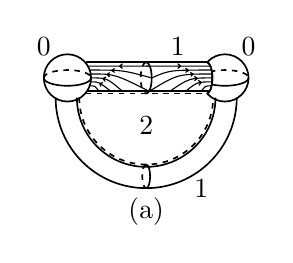
\begin{tikzpicture}[line width=.6, baseline=(base.base)]
        \tikzstyle{dp}=[dash pattern=on 2pt off 2pt]
        \draw (-1,0) circle (0.3);
        \draw (1,0) circle (0.3);
        \draw[dp] (-1.3,0) arc (180:0:0.3 and 0.1);
        \draw (-1.3,0) arc (180:360:0.3 and 0.1);
        \draw[dp] (.7,0) arc (180:0:0.3 and 0.1);
        \draw (.7,0) arc (180:360:0.3 and 0.1);
        \draw[dp,fill=white] (.77,0) ellipse (.07 and .2);
        \fill[white] (.72,0) ellipse (.07 and .2);
        \draw (-.77,.2) -- (.77,.2);
        \draw[dp] (-.77,-.2) -- (.77,-.2);
        \draw (-.75,-.17) -- (.8,-.17);
        \draw (.77,.2) arc (90:-90:.07 and .2);
        \draw (0,.2) arc (90:-90:.07 and .2);
        \draw[dp] (0,.2) arc (90:270:.07 and .2);
        \draw (-1.15,-.25) arc (180:360:1.15);
        \draw[dp] (-.85,-.25) arc (180:360:.85);
        \draw (-.88,-.25) arc (180:360:.88);
        \draw (0,-1.1) arc (90:-90:.05 and .15);
        \draw[dp] (0,-1.1) arc (90:270:.05 and .15);

        \draw[thin] (0,.15) -- (.82,.15) (.4,.18) -- (.44,.15) -- (.4,.12); 
        \draw[thin] (.07,0) .. controls (.3,.1) and (.3,.1) .. (.84,.1) (.5,.125) -- (.54,.095) -- (.5,.07);
        \draw[thin] (.04,-.17) .. controls (.4,.05) and (.4,.05) .. (.85,.05) (.56,.07) -- (.6,.05) -- (.565,.02);
        \draw[thin] (.3,-.17) .. controls (.55,0) and (.55,0) .. (.85,0) (.61,.02) -- (.65,-.005) -- (.615,-.035);
        \draw[thin] (.5,-.17) .. controls (.65,-.05) and (.65,-.05) .. (.85,-.05) (.66,-.03) -- (.7,-.057) -- (.67,-.095);
        \draw[thin] (.7,-.17) .. controls (.75,-.1) and (.75,-.1) .. (.84,-.1);
        
        \draw[thin] (.04,.15) -- (-.74,.15) (-.3,.18) -- (-.34,.15) -- (-.3,.12); 
        \draw[thin] (.07,0) .. controls (-.3,.1) and (-.3,.1) .. (-.72,.1) (-.4,.12) -- (-.44,.095) -- (-.4,.07);
        \draw[thin] (.04,-.17) .. controls (-.4,.05) and (-.4,.05) .. (-.7,.05) (-.46,.067) -- (-.5,.045) -- (-.465,.015);
        \draw[thin] (-.3,-.17) .. controls (-.5,0) and (-.5,0) .. (-.7,0) (-.51,.012) -- (-.55,-.008) -- (-.52,-.045);
        \draw[thin] (-.45,-.17) .. controls (-.6,-.05) and (-.6,-.05) .. (-.7,-.05) (-.55,-.06) -- (-.59,-.07) -- (-.575,-.11);
        \draw[thin] (-.6,-.17) .. controls (-.65,-.1) and (-.65,-.1) .. (-.72,-.1);

        \node at (0,-0.6) {2};
        \node at (.4,0.4) {1};
        \node at (.7,-1.4) {1};
        \node at (1.3,0.4) {0};
        \node at (-1.3,0.4) {0};
        \node (base) at (0,-1.7) {(a)};
    \end{tikzpicture}
    \qquad
    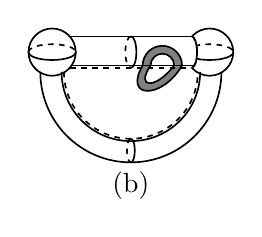
\begin{tikzpicture}[line width=.6, baseline=(base.base)]
        \tikzstyle{dp}=[dash pattern=on 2pt off 2pt]
        \fill[black!50] (.15,-.17) arc (180:0:.25);
        \fill[white] (.25,-.17) arc (180:0:.15);
        \fill[black!50] (.15,-.17) .. controls (-.1,-.6) and (.4,-.6) .. (.65,-.17);
        \fill[white] (.25,-.17) .. controls (.05,-.47) and (.32,-.47) .. (.55,-.17);
        \draw (-1,0) circle (0.3);
        \draw (1,0) circle (0.3);
        \draw[dp] (-1.3,0) arc (180:0:0.3 and 0.1);
        \draw (-1.3,0) arc (180:360:0.3 and 0.1);
        \draw[dp] (.7,0) arc (180:0:0.3 and 0.1);
        \draw (.7,0) arc (180:360:0.3 and 0.1);
        \draw[dp,fill=white] (.77,0) ellipse (.07 and .2);
        \fill[white] (.72,0) ellipse (.07 and .2);
        \draw (-.77,.2) -- (.77,.2);
        \draw[dp] (-.77,-.2) -- (.77,-.2);
        \draw (-.75,-.17) -- (.8,-.17);
        \draw (.77,.2) arc (90:-90:.07 and .2);
        \draw (0,.2) arc (90:-90:.07 and .2);
        \draw[dp] (0,.2) arc (90:270:.07 and .2);
        \draw (-1.15,-.25) arc (180:360:1.15);
        \draw[dp] (-.85,-.25) arc (180:360:.85);
        \draw (-.88,-.25) arc (180:360:.88);
        \draw (0,-1.1) arc (90:-90:.05 and .15);
        \draw[dp] (0,-1.1) arc (90:270:.05 and .15);
        \draw (.15,-.17) arc (180:0:.25);
        \draw (.25,-.17) arc (180:0:.15);
        \draw (.15,-.17) .. controls (-.1,-.6) and (.4,-.6) .. (.65,-.17);
        \draw (.25,-.17) .. controls (.05,-.47) and (.32,-.47) .. (.55,-.17);
        \node (base) at (0,-1.7) {(b)};
    \end{tikzpicture}
    \qquad
    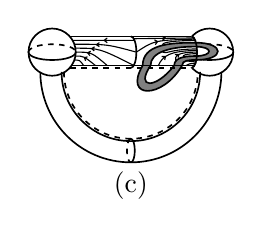
\begin{tikzpicture}[line width=.6, baseline=(base.base)]
        \tikzstyle{dp}=[dash pattern=on 2pt off 2pt]
        \draw (-1,0) circle (0.3);
        \draw (1,0) circle (0.3);
        \draw[dp] (-1.3,0) arc (180:0:0.3 and 0.1);
        \draw (-1.3,0) arc (180:360:0.3 and 0.1);
        \draw[dp] (.7,0) arc (180:0:0.3 and 0.1);
        \draw (.7,0) arc (180:360:0.3 and 0.1);
        \draw[dp,fill=white] (.77,0) ellipse (.07 and .2);
        \fill[white] (.72,0) ellipse (.07 and .2);
        \fill[black!50] (.15,-.17) .. controls (-.1,-.6) and (.4,-.6) .. (.65,-.17);
        \fill[white] (.25,-.17) .. controls (.05,-.47) and (.32,-.47) .. (.55,-.17);
        \fill[black!50] (.15,-.17) .. controls (.15,.1) and (.5,.12) .. (.82,.12)
                        .. controls (1.2,.12) and (1.2,-.1) .. (.82,-.1)
                        .. controls (.75,-.1) and (.65,-.1) .. (.65,-.17);
        \fill[white] (.25,-.17) .. controls (.25,0) and (.5,.07) .. (.82,.07)
                        .. controls (1.05,.07) and (1.05,-.05) .. (.82,-.05)
                        .. controls (.75,-.05) and (.55,-.05) .. (.55,-.17); 
        \draw (-.77,.2) -- (.77,.2);
        \draw[dp] (-.77,-.2) -- (.77,-.2);
        \draw (-.75,-.17) -- (.8,-.17);
        \draw (.77,.2) arc (90:-90:.07 and .2);
        \draw (0,.2) arc (90:-90:.07 and .2);
        \draw (-1.15,-.25) arc (180:360:1.15);
        \draw[dp] (-.85,-.25) arc (180:360:.85);
        \draw (-.88,-.25) arc (180:360:.88);
        \draw (0,-1.1) arc (90:-90:.05 and .15);
        \draw[dp] (0,-1.1) arc (90:270:.05 and .15);
        \draw (.15,-.17) .. controls (-.1,-.6) and (.4,-.6) .. (.65,-.17);
        \draw (.25,-.17) .. controls (.05,-.47) and (.32,-.47) .. (.55,-.17);
        \draw (.15,-.17) .. controls (.15,.1) and (.5,.12) .. (.82,.12)
                        .. controls (1.2,.12) and (1.2,-.1) .. (.82,-.1)
                        .. controls (.75,-.1) and (.65,-.1) .. (.65,-.17);
        \draw (.25,-.17) .. controls (.25,0) and (.5,.07) .. (.82,.07)
                        .. controls (1.05,.07) and (1.05,-.05) .. (.82,-.05)
                        .. controls (.75,-.05) and (.55,-.05) .. (.55,-.17); 
        \draw[thin] (.04,.15) -- (-.74,.15) (-.3,.18) -- (-.34,.15) -- (-.3,.12); 
        \draw[thin] (.07,0) .. controls (-.3,.1) and (-.3,.1) .. (-.72,.1) (-.4,.12) -- (-.44,.095) -- (-.4,.07);
        \draw[thin] (.04,-.17) .. controls (-.4,.05) and (-.4,.05) .. (-.7,.05) (-.46,.067) -- (-.5,.045) -- (-.465,.015);
        \draw[thin] (-.3,-.17) .. controls (-.5,0) and (-.5,0) .. (-.7,0) (-.51,.012) -- (-.55,-.008) -- (-.52,-.045);
        \draw[thin] (-.45,-.17) .. controls (-.6,-.05) and (-.6,-.05) .. (-.7,-.05) (-.55,-.06) -- (-.59,-.07) -- (-.575,-.11);
        \draw[thin] (-.6,-.17) .. controls (-.65,-.1) and (-.65,-.1) .. (-.72,-.1);

        \draw[thin] (.03,.17) -- (.8,.18) (.4,.2) -- (.44,.18) -- (.4,.15); 
        \draw[thin] (.07,0) .. controls (.3,.15) and (.3,.15) .. (.8,.165) (.3,.155) -- (.34,.135) -- (.31,.095);
        \draw[thin] (.4,.08) .. controls (.4,.11) and (.4,.14) .. (.82,.15);
        \draw[thin] (.4,0) .. controls (.45,-.03) and (.5,.04) .. (.84,.04);
        \draw[thin] (.35,-.17) .. controls (.4,-.05) and (.5,.02) .. (.84,.02) (.39,-.055) -- (.44,-.055) -- (.43,-.1);
        \draw[thin] (.57,-.12) .. controls (.55,-.04) and (.6,.0) .. (.84,.0) (.56,-.03) -- (.61,-.03) -- (.6,-.07);
        \draw[thin] (.67,-.06) .. controls (.65,-.04) and (.7,-.02) .. (.84,-.02);
        
        \draw[thin] (.7,-.11) .. controls (.75,-.125) and (.75,-.125) .. (.82,-.125);
        \draw[thin] (.7,-.17) .. controls (.75,-.145) and (.75,-.145) .. (.82,-.145);
        \node (base) at (0,-1.7) {(c)};
    \end{tikzpicture}
    \medskip

    \parbox{96mm}{\small\leftskip=1.5em\parindent=-1.5em
        (a) A $4$-handlebody, where numbers indicate types of handles.
        A $1$-handle is drawn with its expanding field.
        (Of course what is seen here is a $3$-dimensional analogue of the real thing.)
        
        (b) Attach a $3$-handle,
        where the shaded part indicates the image of the attaching map.
        
        (c) Stretch the attaching map using the expanding field,
        and construct a new expanding field on the $1$-handle.
    }
\end{center}}

\begin{lemma}\label{lem:expanded}
    Let $(N,A)$ be a finite relative $n$-handlebody with $i$ handles,
    such that $(N_{i-1},A)$ is good and expanded.
    Then $N_{i-1}$ can be $\epsilon$-slid,
    so that the induced $\epsilon$-perturbation is good and expanded.
\end{lemma}
    
\begin{proof}
    Let $h^\lambda$ denote the handle to be attached,
    and let $\Phi$ denote the attaching map.
    Let $h_j$ denote the handle attached in the $j$-th step.
    Since $(N_{i-1},A)$ is good, we may assume $h_1,\dotsc,h_{i-1}$ are of ascending types.
    
    First we try to slide $\image(\Phi)$ to avoid all handles of type $\geq\lambda$.
    Suppose $\image(\Phi)$ intersects with some $h_{\smash{j}}$ with type $\geq\lambda$,
    and we fix the largest $j$ with this property.
    Then $\image(\Phi)$ does not intersect with $h_{\smash{j+1}},\dotsc,h_{i-1}$.
    By reparametrising $h^\lambda$,
    we may assume that the cobelt $\Phi(\partial D^\lambda\times0)$ avoids the belt $O$ of $h_j$.
    By (\ref{lem:shrink}), we can shrink $\image(\Phi)$
    so that it does not meet $O$.
    We then extend the expanding field on $h_j$ to a small neighbourhood
    in $\partial N_j\cap\partial N_{i-1}$
    that does not meet any handles attached after the $j$-th step,
    and we could slide $\image(\Phi)$ out of $\partial_2h_j$
    using the flow $\phi_t$ of the expanding field for large enough $t$.
    We do this for all $h_j$, in descending order
    until $\image(\Phi)$ finally gets to a (literally) good position,
    i.e.\ within $\partial N_{i'-1}$, where
    $i'$ denotes the step where the first handle of type $\geq\lambda$ is attached.
    
    Our next plan is to do an $\epsilon$-sliding for each $j=i'-1,\dotsc,1$,
    making the corresponding handle expanded at each time.
    By (\ref{cor:transverse}), we may assume that
    $\Phi(\partial\partial_2h^{\lambda})$ is transverse to
    everything in $\Sigma_{i'-1}$,
    while keeping $\image(\Phi)$ disjoint with $h_{i'},\dotsc,h_{i-1}$.
    
    In the $j$-th step,
    let $X$ denote the expanding field on $\partial_2h_j$.
    Let $B\subset\partial N_j$ denote the union of images of attaching maps in steps $j+1,\dotsc,i-1$,
    intersected with $\partial N_j$.
    Let $\Phi'$ denote the composition of $\Phi$ with the previously executed slidings.
    
    Let $S_{j+1},\dotsc,S_i$
    be the boundaries of images of attaching maps
    in the corresponding steps, intersected with $\partial N_j$,
    so that $S_i=\Phi'(\partial\partial_2h^{\smash{\lambda}})\cap\partial N_j$.
    Let $O$ denote the belt of $h_j$.
    Thus the $S_k$ and $B$ are submanifolds possibly with corners,
    and the corners of $B$ are concave.
    By (\ref{lem:extension}) and the remark after it,
    we may extend the $S_k$ that have boundaries a little bit into $B$,
    so that the extended manifolds $\subsup Sk\prime$ are compact,
    and $\partial\subsup Sk\prime\subset B^\circ$ for all $k$.
    %(This can be achieved, for example, by projecting a compact collar of
    %$\partial\partial_2h_k$ in $\partial_2h_k$
    %to a collar of $\partial\partial_2h_k$ in $\partial N_{k-1}$ diffeomorphically,
    %and then projecting it to $\partial N_{k-2},\dotsc,$ and finally to $\partial N_j$.)
    
    By regularity of $(N_{i-1},A)$,
    we may assume $O,\subsup S{j+1}\prime,\dotsc,\subsup Si\prime$ are transverse
    (shrinking a bit the extended part if necessary).
    Thus by (\ref{cor:function}),
    there is a smooth function $f\:\partial N_j\setminus B^\circ\to[0,1]$,
    with $f^{\smash{-1}}(0)=(O\cup\subsup S{j+1}\prime\cup\cdots\cup\subsup Si\prime)\setminus B^\circ$,
    with no critical values other than $0,1$.
    We modify $f$ by letting $f|_B\equiv0$ and $f|_{\image(\Phi')}\equiv0$.
    Now $f$ becomes a smooth function $\partial N_j\to[0,1]$ with $f^{-1}(0)=O\cup B\cup\image(\Phi')$,
    and it has no critical values other than $0,1$.

    We extend $X$ to a compactly supported smooth vector field on $\partial N_j$,
    so that $X|_{B}=0$, and for any $p\in\partial\partial_2h_j$ such that $X_p\neq0$,
    the change of $f$ along the extended part of the flow line of $X$ through $p$ is $<1/2$.
    
    %Notice that any vector field $X'$ that is
    %close enough to $X$ in the sense of (\ref{lem:transversal})
    %is an expanding field.
    %Thus by (\ref{lem:transversal}), we may take such an expanding field $X'$,
    We take a large number $t\in\R$,
    such that the flow $h:=\phi_t$ of $X$ satisfies
    \[h\bigl(f^{-1}([1/2,1])\cap\partial_2h_j\bigr)\cap\partial_2h_j=\emptyset.\]
    By (\ref{cor:transverse}), after performing a small isotopy
    preserving the above condition, keeping $B$ fixed,
    we may assume that $h(\Phi'(\partial\partial_2h^\lambda))$ is transverse to
    everything in $\Sigma_{i-1}$.
    
    Take a metric on $\partial_2h_j$, and put
    \[ Y_p:=\d h(\grad f(h^{-1}(p))). \]
    One verifies that $Y$ is a new expanding field on $\partial_2h_j$, 
    but with respect to $B\cup\image(h\circ\Phi')$ instead of $B$.
    Note that $h$ keeps $B$ fixed.
    Finally we execute the $\epsilon$-sliding induced by $h$.
    
    We have finished the $j$-th step.
    Running over $j=i'-1,\dotsc,1$ gives a desired $\epsilon$-sliding,
    and gives desired expanding fields on all handles except the $i$-th one.
    But the $i$-th handle is trivially done.
    Regularity is preserved throughout the above construction.
\end{proof}

Having done much preparatory work,
we are finally ready to take our final step to proving (\ref{thm-rearrange-weak}),
namely, the concatenation of these infinitely many slidings
given by the preceding lemma.

\begin{proof}[Proof of \textup{(\ref{thm-rearrange-weak})}]
Let $(N,A)$ be a weak relative $n$-handlebody.
We may assume that only one handle is attached in each step.
For each $i\geq0$, we may regard $(N_i,A)$ as a non-weak relative handlebody.
Let $\theta_i$ be a level function on $N_i$ for $i=0,1,\dotsc$,
so that $\theta_i\leq\theta_{i+1}$ for all $i$.
%Denote $\subsup Ni\circ=N_i-\partial N_i$,
%and denote $\Theta(p):=\theta_i(p)$ if $p\in\subsup Ni\circ-\subsup N{i-1}\circ$,
%where $\subsup N{-1}\circ$ is understood to be the empty set.
%Thus $\Theta$ is a function 

Denote $N^1=N$. Note that $(\subsup N11,A)$ is automatically expanded.
By (\ref{lem:expanded}),
$\subsup N11$ can be $1/2$-slid,
so that if we denote by $(N^2,A)$ the induced perturbation,
then $(\subsup N22,A)$ is expanded. 
We continue to $1/4$-slide $\subsup N22$ to get a perturbation $(N^3,A)$ of $(N^2,A)$,
so that $(\subsup N33,A)$ is expanded.
Continuing this process, using $1/2^i$ in the $i$-th step,
we get a commutative grid of maps
\[ \begin{tikzcd}
\subsup N01\ar[r,hook] &\subsup N11\ar[r,hook]\ar[d,"\simeq"] &\subsup N21\ar[r,hook]\ar[d,"\simeq"] &\subsup N31\ar[r,hook]\ar[d,"\simeq"] &\subsup N41\ar[r,hook]\ar[d,"\simeq"] &\cdots\\
\subsup N02\ar[r,hook] &\subsup N12\ar[r,hook] &\subsup N22\ar[r,hook]\ar[d,"\simeq"] &\subsup N32\ar[r,hook]\ar[d,"\simeq"] &\subsup N42\ar[r,hook]\ar[d,"\simeq"] &\cdots\\
\subsup N03\ar[r,hook] &\subsup N13\ar[r,hook] &\subsup N23\ar[r,hook] &\subsup N33\ar[r,hook]\ar[d,"\simeq"] &\subsup N43\ar[r,hook]\ar[d,"\simeq"] &\cdots\rlap,\\
&&&\dots&\dots
\end{tikzcd} \]
where the vertical maps are all diffeomorphisms.
By construction $\subsup Nii$ and $\subsup Ni{i+1}$ are naturally identified,
but note that the identification is not the diffeomorphism (sliding) in the diagram.
We define $\theta_i$ on $\subsup N{\smash{j}}i$ for $i\leq j+1$ to be the
level function inherited from $N_j=\subsup Nj1$.
Thus for $\subsup Nii$ and $\subsup Ni{i+1}$,
their functions $\theta_i$ are the same under the natural identification.

We define a good weak relative $n$-handlebody $(N',A)$ 
by $\subsup Ni\prime:=\subsup Nii$, 
and the inclusion maps being $\subsup Nii=\subsup Ni{i+1}\hookrightarrow\subsup N{i+1}{i+1}$.
This is \emph{not} the map in the above diagram!
But for $p\in\subsup Nii\subset\subsup N{i+1}{i+1}$, we still have
$\theta_i(p)\leq\theta_{i+1}(p)$.
We will show that $N$ is diffeomorphic to $N'$. 

Consider the (not commutative) diagram
\[ \begin{tikzcd}
N_1\ar[d,equals]\ar[r,hook] &N_2\ar[d,"\simeq"]\ar[r,hook] &N_3\ar[d,"\simeq"]\ar[r,hook] &\cdots\\
\subsup N11\ar[r,hook] &\subsup N22\ar[r,hook] &\subsup N33\ar[r,hook] &\cdots\rlap,
\end{tikzcd}\eqno(*) \]
where the vertical maps are as in the above grid-like diagram.
By comparing the above two diagrams, the square
\[ \begin{tikzcd}
N_i\ar[r,hook]\ar[d,"\simeq"] &N_{i+1}\ar[d,"\simeq"]\\
\subsup Nii\ar[r,hook] &\subsup N{i+1}{i+1}
\end{tikzcd} \]
commutes for some $p\in N_i$
if and only if $p$ is fixed by the sliding $\subsup Nii\to\subsup Ni{i+1}$.
This happens whenever $\theta_i(p)>1/2^i$. Thus for
\[ U_i:=\{p\in N_i\mid\theta_i(p)>1/2^i\}, \]
the diagram $(*)$ commutes after the $i$-th square.
Thus we have an induced diffeomorphism of $U_i$ onto a subset of $N'$.
Since $N=\bigcup_{i=1}^\infty U_i$, we have an induced map $\phi\:N\to N'$
which is a diffeomorphism onto its image.
Clearly $\phi$ is also surjective since $N'=\bigcup_{i=1}^\infty\image(U_i\to N')$.
Thus $\phi$ is a diffeomorphism. 
\end{proof}

\subsection{The cancellation theorem}

We first state the cancellation theorem
for finite handlebodies.

\begin{theorem}[Cancellation, finite case]\label{thm:cancel}
Let $N=A\cup_{\Phi_1}h^\lambda\cup_{\Phi_2}h^{\lambda+1}$ be a relative handlebody with $2$ handles.
If the cobelt of $h^{\lambda+1}$ and the belt of $h^\lambda$ intersect transversely
at precisely one point, then $N$ is diffeomorphic to $A$.
This diffeomorphism can be taken to be fixed on any closed subset of $A\setminus\image(\Phi_1)\setminus\image(\Phi_2)$.
\end{theorem}

\begin{proof}
\cite[Theorem~5.4.3]{wall} or \cite[Theorem~3.34]{matsu}.
\end{proof}

For convenience, we introduce the following terminology.
In a good relative handlebody, a pair of $\lambda$- and $(\lambda+1)$-handles is called a
\term{cancelling pair}, if the cobelt of the $(\lambda+1)$-handle
and the belt of the $\lambda$-handle intersect transversely
at precisely one point. 
The $(\lambda+1)$-handle will be called the \term{canceller},
and the $\lambda$-handle will be called the \term{cancellee}.

We say that we can \term{cancel} a set $S$ of handles from a weak relative handlebody $(N,A)$,
if $N$ is diffeomorphic to a weak relative handlebody,
whose $\lambda$-handles correspond to
the $\lambda$-handles of $N$ that are not in $S$,
and the combinatorics concerning which handles are attached to other handles should not change,
except that a handle attached to a cancelled handle may get attached to
a handle which a cancelled handle was attached to.

\begin{theorem}[Cancellation, infinite case] \label{thm:cancel-infinite}
Let $(N,A)$ be a weak relative handlebody whose handles are attached one at a time,
and let $S$ be a set of handles consisting of cancelling pairs
that do not have handles in common,
such that every canceller in $S$ is attached immediately after its cancellee.
Then $S$ can be cancelled.
\end{theorem}

\begin{proof}
We will construct a new weak handlebody $N'$ diffeomorphic to $N$,
with the desired property.

Let $\subsup N0\prime:=N_0=A$, and let $\theta_0$ be a level function on it.
Let $\phi_0\:N_0\to\subsup N0\prime$ be a diffeomorphism.
As we construct $N'$, we will construct diffeomorphisms $\phi_i\:N_i\to\subsup Ni\prime$,
and level functions $\theta_i$ on $\subsup Ni\prime$,
such that $\theta_i\leq\theta_{i+1}$ on $\subsup Ni\prime$.
This will be implicit in the below construction.

In the $i$-th step, if the $i$-th handle of $N$ is not a canceller or a cancellee,
then we attach a same handle to $N'$ according to $\phi_{i-1}$,
and let $\phi_i$ be the induced diffeomorphism.
If it is a cancellee (followed by its canceller),
then we will not attach handles to $N'$ in the $i$-th and $(i+1)$-th steps.
Instead, we construct by (\ref{thm:cancel}) a diffeomorphism $\phi_{i+1}$ to form a (not commutative) diagram
\[ \begin{tikzcd}
N_{i-1}\ar[d,"\phi_{i-1}"',"\simeq"]\ar[r,hook] &N_i\ar[r,hook] &N_{i+1}\ar[d,"\phi_{i+1}"',"\simeq"]\\
\subsup N{i-1}\prime\ar[r,equals] &\subsup Ni\prime\ar[r,equals] &\subsup N{i+1}\prime\rlap.
\end{tikzcd} \]
By the last statement of (\ref{thm:cancel}), we may require the diagram to commute in
$\subsup U{i-1}\prime:=\{p\in\subsup N{i-1}\prime\mid\theta_{i-1}(p)>1/2^{i-1}\}$.
We take a new level function $\theta_{i+1}$ on $\subsup N{i+1}\prime$,
so that for all $p\in\subsup N{i-1}\prime$, we have
\[\theta_{i+1}(p)\geq\theta_{i-1}(p)\quad\text{and}\quad
\theta_{i+1}(p)\geq\theta_{i-1}(\phi_{i+1}\circ\subsup{\phi}{i-1}{-1}(p)).\]
By a same argument as before, we have a colimit map from $N'$ to $N$,
which is an embedding. It is surjective by the choice of the functions $\theta_i$.
\end{proof}

We have now completed the proof of our two 
main theorems. They can be combined to obtain
the following result, which simplifies weak handlebodies.

\begin{definition}
Let $n\geq m\geq0$ be integers. An \term{$(n,m)$-handlebody} is an $n$-handlebody
whose handles are of type $0,1,\dotsc,m$. \varqed
\end{definition}

\begin{corollary}\label{prop:0-handle}
Every connected finite handlebody is diffeomorphic to
a handlebody with only one $0$-handle.
Every connected weak handlebody is diffeomorphic to
a good weak handlebody with only one $0$-handle.
\end{corollary}

\begin{proof}
For the finite case, we may suppose that the handlebody is good by (\ref{thm-rearrangement}).
Thus it suffices to prove the statement for an $(n,1)$-handlebody.
Consider a graph with vertices corresponding to the $0$-handles
and edges corresponding to the $1$-handles.
Then this graph is connected.
Taking a maximal tree of this graph,
we may assume the handlebody is simply connected
(by discarding the $1$-handles not in the tree).
Thus the result follows from (\ref{thm:cancel}),
by cancelling the $0$- and $1$-handles a pair at a time.

For the weak case, we suppose that the handlebody is good by (\ref{thm-rearrange-weak}).
We construct a graph and take a maximal tree in the same way,
and the statement follows from (\ref{thm:cancel-infinite}).
\end{proof}


\section{陈--Weil 理论 (上)} \label{sect-5}

从这一节开始, 我们从一个全新的角度出发, 来重新建造示性类的理论.
这个角度就是微分几何的观点.
我们将研究流形上的向量丛和主丛,
并通过它们的几何量, 即曲率形式, 来定义示性类.
这样定义出的示性类是一些闭微分形式, 其 de~Rham 上同调类就是我们之前研究的示性类.
这一套理论被称为\term{陈--Weil 理论}.

通过这种方式, 我们能通过流形的几何量, 来计算它的拓扑.
这种想法的一个经典的形式是 \term{Gauß--Bonnet 公式}:
对于二维可定向紧 Riemann 流形 $M$, 我们有
\[ \int_M K \, d S = 2 \uppi \, \chi (M), \]
其中 $K$ 是 Gauß 曲率, $dS$ 是面积元.
我们可以把陈--Weil 理论看作这个公式的一般形式.

从本节开始, 所有流形都默认是光滑、不带边的.


\subsection{联络和曲率}

\begin{definition}
    设 $M$ 是流形. $M$ 上的一个\term{光滑向量丛} (smooth vector bundle)
    是指一个 (实或复) 向量丛
    \[ E \to M, \]
    其转移映射都是 (从 $M$ 的开集出发的) 光滑映射.
    此时, $E$ 具有一个自然的光滑结构.
\end{definition}

在下面的讨论中, 设 $E \to M$ 是一个光滑 $\bbK$-向量丛, 其中 $\bbK = \bbR, \bbC$.
设 $M$ 的维数为 $n$, $E$ 的秩为 $m$.
我们用记号 $\Gamma (E)$ 表示 $E$ 的所有光滑截面的集合.

向量丛 $E$ 上的一个\term{联络}就是一个将
$E$ 的每个纤维与它周围的纤维对齐的方法.
如果我们知道如何对齐这些纤维, 我们就可以对 $E$ 的截面取方向导数.
这解释了下面的定义.

\begin{definition}
    $E$ 上的一个\term{联络} (connection) 是一个映射
    \[ \begin{aligned}
        \nabla \: \Gamma (TM) \otimes \Gamma (E) &\to \Gamma (E), \\
        (X, \ s) &\mapsto \nabla_X s, 
    \end{aligned} \]
    满足以下公理:
    \begin{itemize}
        \item
            $\nabla_X s$ 关于 $X$ 是 $C^\infty (M)$-线性的,
            关于 $s$ 是 $\bbK$-线性的.
        \item (\term{Leibniz 法则})
            如果 $X \in \Gamma (TM)$, $s \in \Gamma (E)$, $f \in C^\infty (M, \bbK)$, 那么
            \[ \nabla_X (fs) = (Xf) \, s + f \, \nabla_X s. \]
            换言之, 作为 $E$-取值的 $1$-形式 (即 $T^* M \otimes E$ 的截面), 有
            \[ \nabla (fs) = (df) \, s + f \, \nabla s. \]
    \end{itemize}
    如果 $E$ 的纤维带有 (Euclid 或 Hermite) 度量, 我们还可以要求:
    \begin{itemize}
        \item (\term{Leibniz 法则})
            如果 $X \in \Gamma (TM)$, $s_1, s_2 \in \Gamma (E)$, 那么
            \[ X \, \langle s_1, s_2 \rangle =
                \langle \nabla_X s_1, s_2 \rangle + \langle s_1, \nabla_X s_2 \rangle. \]
    \end{itemize}
    此时, $\nabla$ 称为一个\term{度量联络} (metric connection).
\end{definition}

在实际的计算中, 上面的定义常常是不好用的.
我们将联络的局部信息提取出来, 成为一些微分形式, 以便于直接计算截面的方向导数.

\begin{definition}
    设开集 $U \subset M$ 上 $E$ 平凡, 即 $E |_U \simeq U \times \bbK^m$.
    设 $e_1, \dotsc, e_m$ 是由 $\bbK^m$ 的基给出的 $E |_U$ 的 $m$ 个截面. 设
    \[ \nabla e_j = \omega_j^i e_i, \]
    其中 $\omega_j^i \in \Omega^1 (U, \bbK)$.
    这 $m^2$ 个 $1$-形式称为联络 $\nabla$ 的\term{联络形式} (connection form).
    我们可以把 $\omega$ 看作
    \[ \Omega^1 \bigl( U, \ \End (E) \bigr) =
        \Gamma \bigl( T^* U \otimes \End (E) \bigr) \]
    的截面, 因为它是由 $m^2$ 个 $1$-形式构成的矩阵, 也就是一个取值为矩阵的 $1$-形式.
\end{definition}

需要注意的是, $\omega$ 并不能定义出整个 $M$ 上的 $1$-形式,
因为它不符合 $1$-形式的坐标变换法则.

\begin{remark}
    为了直观地理解联络形式, 我们把 $\End (E)$ 与 Lie 代数 $\gl (E)$ 等同起来.
    对任意向量场 $X \in \Gamma (TM)$, 局部截面
    \[ \omega (X) \in \Gamma \bigl( U, \gl (E) \bigr) \]
    给出了从某一点 $x \in U$ 出发, 沿着 $X$ 的方向走无穷小的距离时,
    得到 $E$ 的纤维的无穷小自同构, 即 $\GL (E_x)$ 的一个无穷小元素.
    这个自同构就是由联络所指定的将相邻纤维等同起来的方法.
    
    事实上, 对于一般的 Lie 群 $G$, 我们也可以谈论 $G$-主丛上的联络,
    其联络形式是取值于 Lie 代数 $\mathfrak{g}$ 的形式.
    为了对用户友好, 我们在行文中总是取 $G = \GL (n)$,
    但一般的 Lie 群的情况其实大同小异. \varqed
\end{remark}

现在, 我们就可以在局部上计算出截面的方向导数了:
\[ \nabla_X (s^j e_j) = X^\alpha (\partial_\alpha s^j) \, e_j 
    + s^j X^\alpha (\omega_j^i)_\alpha \, e_i, \]
其中希腊字母表示流形方向的坐标, 罗马字母表示纤维方向的坐标.
记号 $(\omega_j^i)_\alpha$ 表示 $1$-形式 $\omega_j^i$ 的 $\alpha$-分量.
注意到, $\omega$ 描述了联络给出的方向导数和局部坐标下的导数的差异.

\begin{definition}
    联络 $\nabla$ 的\term{曲率形式} (curvature form)
    是 $m^2$ 个 $2$-形式, 定义为
    \[ \Omega_j^i = d \omega_j^i + \omega_k^i \wedge \omega_j^k. \]
    这个公式可以简写成
    \[ \Omega = d \omega + \omega \wedge \omega, \]
    其中 $\Omega$ 是 $\End (E)$ 取值的 $2$-形式,
    记号 $\omega \wedge \omega$ 的意思是把两个矩阵相乘,
    但矩阵的元素都是 $1$-形式, 这些元素相乘的方法是做外积.
\end{definition}

由于记号约定不同, 一些作者会把这个公式写成
\[ \Omega = d \omega - \omega \wedge \omega. \]
出现这种现象的原因是, 这些作者的上下标与我们相反,
所以我们的 $\omega_k^i \wedge \omega_j^k$
相当于这些作者的 $-\omega_k^j \wedge \omega_i^k$.

之所以将 $\Omega$ 称为曲率形式, 是因为对 $X, Y \in \Gamma (TM)$, 有
\begin{equation} \label{eq-5-omega-equals-r}
    \Omega (X, Y) = R (X, Y) \quad \in \Gamma (\End (E)),
\end{equation} 
其中 $R (X, Y) = \nabla_X \nabla_Y - \nabla_Y \nabla_X - \nabla_{[X, Y]}$
是 Riemann 曲率张量. 读者可以验证这个公式.

实际上, 这个公式还说明, 虽然 $\Omega$ 是局部定义的,
但它是整个 $M$ 上的一个张量. 这个性质是联络形式所不具有的.

\begin{proposition}
    $\Omega$ 定义了整个 $M$ 上的一个 $2$-形式:
    \[ \Omega \in \Omega^2 \bigl( M, \End (E) \bigr). \thmqedhere \]
\end{proposition}

曲率形式还有另一种诠释.
给定 $E$ 上的一个联络, 我们不仅能对 $E$ 的截面求方向导数,
也能对 $E$-取值的微分形式求方向导数:

\begin{definition}
    设 $s \in \Gamma (E)$, $\alpha \in \Omega^\bullet (M)$.
    通过 Leibniz 法则, 我们定义
    \[ \nabla ( s \otimes \alpha ) = \nabla s \wedge \alpha + s \otimes d \alpha. \]
    这样就定义了 $E$-取值的微分形式的方向导数.
\end{definition}

于是, 我们有一系列映射
\[ \Omega^0 (M, E) \overset{\nabla}{\longrightarrow}
    \Omega^1 (M, E) \overset{\nabla}{\longrightarrow} 
    \Omega^2 (M, E) \overset{\nabla}{\longrightarrow} \cdots. \]
对于 $s \in \Gamma (E)$, 我们有
\begin{equation} \label{eq-5-curv-nabla-sq}
    \nabla^2 s = \Omega s \quad \in \Omega^2 (M, E).
\end{equation}
这个性质常常被简写为 $\Omega = \nabla^2$. 请读者验证这个等式.

最后, 我们有一个著名的关于曲率形式的等式, 其验证留给读者.

\begin{proposition} [Bianchi 恒等式] \label{thm-5-bianchi}
    在局部上, 我们有
    \[ d \Omega = [ \Omega, \omega ], \]
    其中 $[ \Omega, \omega ] = \Omega \wedge \omega - \omega \wedge \Omega$. \qed
\end{proposition}


\subsection{曲率不变量}

下面, 我们从一个联络的曲率 $2$-形式中提取出一些不变量,
这些不变量不依赖于联络的选取.

\begin{definition}
    $n$ 阶矩阵的\term{不变多项式} (invariant polynomial)
    是指一个函数
    \[ P \: \operatorname{M}_{n \times n} (\bbC) \to \bbC, \]
    它是 $n^2$ 个矩阵元的多项式, 并满足对任意矩阵 $A$ 和可逆矩阵 $T$, 有
    \[ P (TAT^{-1}) = P(A). \]
\end{definition}

\begin{exercise} \label{ex-5-inv-poly}
    设 $P$ 是 $n$ 阶矩阵的不变多项式. 
    则 $P$ 一定是矩阵的 $n$ 个特征值的对称多项式,
    由此推出 $P$ 一定具有
    \[ P (A) = p ( \tr A, \ \tr A^2, \ \dotsc, \ \tr A^n ) \]
    的形式, 其中 $p$ 是多项式. \varqed
\end{exercise}

设 $E \to M$ 是光滑复向量丛, 带有联络 $\nabla$.
一个不变多项式给出了向量丛 $\End (E)$ 的每个纤维到 $\bbC$ 的函数,
因为其取值不依赖于基的选取, 只依赖于线性算子的特征值.
这个函数可以把 $\End (E)$-取值的微分形式变成普通的微分形式.

设 $P$ 是不变多项式. 我们将它作用在曲率 $2$-形式 $\Omega$ 上, 得到一个形式
\[ P (\Omega) \in \Omega^{2 \bullet} (M, \bbC). \]
我们将证明, 这个微分形式是闭形式, 且它给出的 de~Rham 上同调类不依赖于联络的选取.

\begin{proposition}
    $P (\Omega)$ 是闭形式.
\end{proposition}

\begin{proof}
    将 $P$ 写成 (\ref{ex-5-inv-poly}) 的形式.
    因为闭形式的外积仍然是闭形式, 所以, 我们只需证明
    \[ d \tr \Omega^k = 0 \quad (k = 0, 1, \dotsc, m). \]
    而由 Bianchi 恒等式 (\ref{thm-5-bianchi}), 由归纳法不难证明
    \[ d \Omega^k = [ \Omega^k, \omega ] \quad (k = 0, 1, \dotsc). \]
    因此,
    \[ d \tr \Omega^k = \tr d \Omega^k
        = \tr {} [ \Omega^k, \omega ] = 0. \qedhere \]
\end{proof}

\begin{proposition} \label{thm-5-conn-indep}
    上同调类 $[P (\Omega)] \in H^{2 \bullet} (M; \bbC)$
    不依赖于联络 $\nabla$ 的选取.
\end{proposition}

\begin{proof}
    设 $\nabla^0, \nabla^1$ 是 $E$ 上的两个联络.
    考虑向量丛 $E \times \bbR \to M \times \bbR$, 带有联络
    \[ \nabla = t \widetilde{\nabla} ^1 + (1-t) \widetilde{\nabla} ^0, \]
    其中 $\widetilde{\nabla} ^i$ ($i = 1, 2$)
    是 $E \times \bbR$ 上的联络,
    使得截面沿 $E$ 方向的导数由 $\nabla^i$ 给出, 
    沿 $\bbR$ 方向的导数由普通的导数给出.
    换言之, $\widetilde{\nabla} ^i$ 是将
    $\nabla^i$ 的联络 $1$-形式沿着投影映射拉回,
    所定义的 $E \times \bbR$ 上的联络.
    
    记 $i_0, i_1 \: M \hookrightarrow M \times \bbR$ 为含入映射,
    其 $\bbR$-分量分别为 $0$ 和 $1$. 记 $\Omega^0, \Omega^1$
    分别为 $\nabla^0, \nabla^1$ 的曲率形式. 则
    \[ [ P (\Omega^0) ] = i_0^* \, [ P (\Omega) ]
        = i_1^* \, [ P (\Omega) ] = [ P (\Omega^1) ], \]
    因为 $i_0, i_1$ 是同伦的映射.
\end{proof}

这一系列结论表明, 对每个不变多项式 $P$,
上同调类 $[ P (\Omega) ]$ 给出了复向量丛的拓扑不变量.
事实上, 这些不变量就是我们熟悉的陈类, 以及陈类的多项式.
在下面几个小节中, 我们将导出这些不变量与陈类的对应关系.

\begin{definition}
    设 $1 \leq k \leq n$ 为整数. 对 $n$ 阶复矩阵 $A$, 我们记
    \[ \sigma_k (A) = \sum_{1 \leq i_1 < \dotsc < i_k \leq n}
        \lambda_{i_1} \cdots \lambda_{i_k} \]
    为 $A$ 的 $n$ 个特征值的第 $k$ 个初等对称多项式,
    它是一个不变多项式.
\end{definition}

我们即将证明, $E$ 的陈类由下面的公式给出:
\[ c_k (E) = \frac {1} {(2 \uppi \upi)^k} \, [ \sigma_k (\Omega) ]. \]


\subsection{第一陈类}

我们首先考虑最简单的情况, 即线丛的第一陈类.

\begin{theorem} \label{thm-5-c1}
    设 $E \to M$ 是光滑复线丛, 带有联络 $\nabla$ 和曲率形式 $\Omega$. 则
    \[ c_1 (E) = \frac {1} {2 \uppi \upi} \, [ \Omega ]. \]
\end{theorem}

\begin{proof}
    设 $E$ 的分类映射是
    \[ \phi \: M \to \bbC \upP^\infty, \]
    其中 $\bbC \upP^\infty$ 是复线丛的分类空间.
    由胞腔近似定理, $\phi$ 的像可以同伦到 $\bbC \upP^\infty$ 的一个有限维子 CW 复形中.
    因此, 在同伦意义下, 我们可以将 $\phi$ 视为一个映射
    \[ \phi \: M \to \bbC \upP^N \quad (N > 0). \]
    在同伦意义下, 我们还可以假定 $\phi$ 是光滑映射 (例如利用磨光).
    
    我们知道 $H^2 ( \bbC \upP^N; \bbC ) \simeq \bbC \cdot c_1$,
    其中 $c_1$ 是自言线丛 $\scrO (-1)$ 的第一陈类. 
    因此, 存在常数 $\alpha \in \bbC$, 使得 
    \[ [ \Omega ] = \alpha \, c_1, \]
    其中 $\Omega$ 是 $\scrO (-1)$ 的曲率形式.
    
    我们有 $E \simeq \phi^* \scrO (-1)$. 
    我们可以把 $\scrO (-1)$ 的联络 $1$-形式通过 $\phi$ 拉回,
    得到 $E$ 上的联络, 其曲率形式是 $\Omega^E = \phi^* \Omega$. 从而
    \[ [ \Omega^E ] = \alpha \, \phi^* c_1 = \alpha \, c_1 (E). \]
    
    最后, 我们来确定常数 $\alpha$.
    
    我们改变记号: 设 $M$ 是二维可定向 Riemann 流形,
    $E \to M$ 是 $M$ 的切丛. 则 $E$ 可以自然地被看作一个复线丛,
    因为乘以 $\upi$ 的操作就是逆时针旋转 $90^\circ$.
    在 $E$ (作为实向量丛) 上有一个自然的度量联络, 
    即 Levi-Civita 联络, 我们记作 $\nabla^{\bbR}$.
    
    取 $E$ 的局部截面 $e_1$, 满足 $|e_1| \equiv 1$, 并记 $e_2 = \upi e_1$. 
    以它们为局部坐标, 则 $\omega_1^1 = 0$, 因为对任何向量场 $X$,
    有 $\nabla^{\bbR}_X e_1 \perp e_1$. 这说明
    \[ \nabla^{\bbR} e_1 = \omega_1^2 \otimes e_2
        = \upi \omega_1^2 \otimes e_1. \]
    我们定义 $E$ (作为复向量丛) 上的联络 $\nabla^{\bbC}$ 如下:
    对任何截面 $s$, 定义
    \[ \nabla^{\bbC} s = \nabla^{\bbR} s \quad \in \Omega^1 (M, E). \]
    则 $\nabla^{\bbC}$ 确实是联络,
    因为联络的本质就是把邻近的纤维对齐的方法,
    而 $\nabla^{\bbR}$ 保持了纤维上的内积, 从而也是 $\bbC$-线性的. 
    
    现在, 我们有 $\nabla^{\bbC} e_1 = \upi \omega_1^2 \otimes e_1$.
    因此, $\nabla^{\bbC}$ 的联络形式是
    \[ \omega^{\bbC} = \upi \omega_1^2, \]
    这里我们省去了 $\omega^{\bbC}$ 的上下标 $1$. 从而, $\nabla^{\bbC}$ 的曲率形式是
    \[ \Omega^{\bbC} = \upi \Omega_1^2. \]
    
    为了确定 $\alpha$ 的值, 我们取 $M = S^2$ 为标准的单位球面.
    一方面, 我们有
    \[ \int_{S^2} \Omega^{\bbC} = \alpha \, \langle c_1 (TM), \ [M] \rangle
        = \alpha \, \langle e(TM), \ [M] \rangle = 2 \alpha, \]
    而另一方面, 由 (\ref{eq-5-omega-equals-r}),
    在开集 $U \subset S^2$ 上的局部坐标中, 有
    \[ \int_U \Omega^{\bbC} = \upi \int_U \Omega_1^2
        = \upi \int_U K \, dS = \upi \cdot (U \text{ 的面积}), \]
    其中 $K$ 是 Gauß 曲率, $S$ 是面积元. 因此,
    \[ 2 \alpha = \upi \cdot (S^2 \text{ 的面积}) = 4 \uppi \upi, \]
    从而 $\alpha = 2 \uppi \upi$.
\end{proof}

现在, 我们已经知道了 $\alpha$ 的值.
因此, 在上面的证明最后, 如果我们把 $S^2$ 换成别的流形,
就可以导出 Gauß--Bonnet 公式.

\begin{corollary} [Gauß--Bonnet 公式]
    设 $M$ 是二维可定向紧 Riemann 流形. 则
    \[ \int_M K \, d S = 2 \uppi \, \chi (M), \]
    其中 $K$ 是 Gauß 曲率, $dS$ 是面积元. \qed
\end{corollary}


\subsection{陈形式}

\begin{theorem}
    设 $E \to M$ 是光滑复向量丛, 带有联络 $\nabla$ 和曲率形式 $\Omega$. 则
    \[ c_k (E) = \frac {1} {(2 \uppi \upi)^k} \, [ \sigma_k (\Omega) ]. \]
    因此, $2k$-形式 $(2 \uppi \upi)^{-k} \sigma_k (\Omega)$
    称为 $E$ 的第 $k$ 个\term{陈形式}.
\end{theorem}

\begin{proof}
    \allowdisplaybreaks
    考虑 $m$ 阶矩阵的不变多项式 $P$, 定义为
    \[ P (A) = \sum _{k=0} ^m \frac {1} {(2 \uppi \upi)^k} \, \sigma_k (A)
        = \det {} \Bigl( I + \frac {A} {2 \uppi \upi} \Bigr), \]
    其中 $I$ 表示单位矩阵. 这个不变多项式对应着向量丛的全陈类.
    
    我们先考虑 $E = L_1 \oplus \cdots \oplus L_m$ 是若干线丛的直和的情况.
    我们在每个 $L_i$ 上取联络 $\nabla^i$, 然后定义 $E$ 上的联络
    $\nabla = \bigoplus_i \nabla^i$. 换言之, $\nabla$ 的联络 $1$-形式是
    \[ \omega = \operatorname{diag} (\omega^1, \dotsc, \omega^m), \]
    即由各 $\nabla^i$ 的联络形式构成的对角矩阵. 从而, $\nabla$ 的曲率形式是
    \[ \Omega = \operatorname{diag} (\Omega^1, \dotsc, \Omega^m). \]
    因此,
    \begin{align*}
        P (\Omega) 
        &= \det {} \biggl[ \operatorname{diag} {} \biggl(
            1 + \frac {\Omega^1} {2 \uppi \upi}, \ \dotsc, \ 
            1 + \frac {\Omega^m} {2 \uppi \upi} \biggr) \biggr] \\
        &= P (\Omega^1) \cdots P (\Omega^m) \\
        &= c (L_1) \cdots c (L_m) \\
        &= c (E),
    \end{align*} 
    其中第三个等号使用了 (\ref{thm-5-c1}).
    
    对于一般的情况, 使用分裂原理不难完成证明.
    当然, 我们需要的是光滑版本的分裂原理,
    但其证明与拓扑版本的分裂原理是完全相同的.
\end{proof}

在上面的证明中, 我们也得到了计算全陈类的公式. 
我们将这个公式和计算陈特征的公式一并列出:

\begin{corollary} \label{thm-5-total-chern}
    设 $E \to M$ 是光滑复向量丛, 带有联络 $\nabla$ 和曲率形式 $\Omega$. 则
    \[ \begin{aligned}[b]
        c (E) &= \biggl[ \det {} \Bigl( I + \frac {\Omega} {2 \uppi \upi} \Bigr) \biggr]
            && \in H^{2 \bullet} (M; \bbC), \\
        \ch (E) &= [ \tr \upe^{\Omega / 2 \uppi \upi} ]
            && \in H^{2 \bullet} (M; \bbC).
    \end{aligned} \thmqedhere \]
\end{corollary}

实向量丛的 Понтрягин 类是通过陈类定义的.
因此, 我们也能将 Понтрягин 类用微分形式表示出来.

\begin{corollary}
    设 $E \to M$ 是光滑实向量丛, 带有联络 $\nabla$ 和曲率形式 $\Omega$. 则
    \[ p_k (E) = \frac {1} {(2 \uppi)^{2k}} \, [ \sigma_{2k} (\Omega) ]. \]
    因此, $4k$-形式 $(2 \uppi)^{-2k} \sigma_{2k} (\Omega)$
    称为 $E$ 的第 $k$ 个 \term{Понтрягин 形式}.
\end{corollary}

\begin{proof}
    证明中唯一不太显然的地方是:
    $E$ 上的联络可以自然地诱导 $E \otimes \bbC$ 上的联络,
    二者的联络形式相等, 从而曲率形式也相等.
\end{proof}


\subsection{陈--Gauß--Bonnet 公式}

利用上面的理论, 我们可以证明 Gauß--Bonnet 公式向高维流形的推广,
它把流形的 Euler 数表示为曲率不变量的积分.
事实上, 奇数维紧流形的 Euler 数总是 $0$,
而对偶数维流形来说, 切丛的 Euler 类是最高阶 Понтрягин 类的平方根.
因此, 我们只要描述清楚这个平方根, 就能获得计算 Euler 数的公式.

\begin{definition}
    设 $V$ 是已定向的 $n$ 维欧氏向量空间, 
    $e_1, \dotsc, e_n$ 为一组与定向相符的标准正交基. 线性映射
    \[ T \: {\wedge^\bullet \, V} \to \bbR \]
    定义如下: $T (e_1 \wedge \cdots \wedge e_n) = 1$, $T (\wedge^{<n} \, V) = 0$.
    映射 $T$ 称为 \term{Березин 积分}.\footnote{英文转录为 Berezin.}
\end{definition}

\begin{definition}
    沿用上面的记号, 设 $A \in \wedge^2 \, V$, 可以看作一个反对称矩阵. 定义
    \[ \exp^{\wedge} A = \sum _{k=0} ^\infty \frac {A^{\wedge k}} {k!}
        \quad \in \wedge^\bullet \, V. \]
    事实上, 这个求和是有限和.
    我们定义 $A$ 的 \term{Pfaff 值} (Pfaffian) 为
    \[ \operatorname{pf} A = T ( \exp^{\wedge} A ). \]
\end{definition}

Pfaff 值的重要性质是, 它是行列式的平方根, 
同时也是矩阵元素的多项式.

\begin{proposition}
    沿用上面的记号, 将 $A$ 看成反对称矩阵, 我们有
    \[ (\operatorname{pf} A)^2 = \det A. \]
\end{proposition}

\begin{proof}
    通过正交相似变换, $A$ 可以化为标准型, 即分块对角矩阵
    \[ A = \operatorname{diag} (B_1, \dotsc, B_k, 0, \dotsc, 0), \quad
        B_i = \Bigl( \begin{smallmatrix} 0 & a_i \\ -a_i & 0 \end{smallmatrix} \Bigr). \]
    我们记 $A = A_1 + \cdots + A_k$, 
    其中 $A_i$ 是将 $A$ 中除了 $B_i$ 外的部分都清零得到的矩阵. 则
    \[ A_i = a_i \, \bigl( e_{2i-1} \otimes e_{2i} - e_{2i} \otimes e_{2i-1} \bigr)
        = a_i \, (e_{2i-1} \wedge e_{2i}), \]
    其中 $e_i$ 表示第 $i$ 个基向量. 
    因此, 若 $k = n/2$, 则
    \begin{align*}
        T (\exp^\wedge A) 
        &= \frac {1} {k!} \, T (A^{\wedge k}) \\
        &= \frac {1} {k!} \, T ( k! \, A_1 \wedge \cdots \wedge A_k ) \\
        &= a_1 \cdots a_k \, T ( e_1 \wedge \cdots \wedge e_n ) \\
        &= a_1 \cdots a_k.
    \end{align*}
    而 $\det A = a_1^2 \cdots a_k^2$.
    若 $k < n/2$, 则 $T (\exp^\wedge A) = 0$.
\end{proof}

有了 Pfaff 值, 我们可以对反对称矩阵的行列式开平方根.
对于度量联络而言, 曲率形式确实是反对称的:

\begin{proposition} \label{thm-5-curv-antisym}
    设 $E \to M$ 是光滑实向量丛, 具有 Euclid 度量. 设 $\nabla$ 是度量联络.
    则曲率形式 $\Omega$ 是取值于 $\mathfrak{so}(E)$ 的 $2$-形式,
    即在标准正交基下表示为反对称矩阵: $\Omega_i^j = -\Omega_j^i$.
\end{proposition}

\begin{proof}
    事实上, 在局部坐标系中, 联络形式也是反对称的, 即满足若 $e_1, \dotsc, e_m$
    是 $E$ 的局部截面, 它们构成 $E$ 的每个纤维的标准正交基, 则以它们为局部坐标,
    有 $\omega_i^j = -\omega_j^i$. 这是因为对任何向量场 $X$, 有
    \[ 0 = X \langle e_i, \ e_j \rangle
        = \langle \nabla_X e_i, \ e_j \rangle + \langle e_i, \ \nabla_X e_j \rangle 
        = \omega_i^j (X) + \omega_j^i (X). \qedhere \]
\end{proof}

因此, 我们可以对得到偶数维流形切丛的最高阶 Понтрягин 类开平方, 得到 Euler 类的表达式.

\begin{theorem} [陈--Gauß--Bonnet 公式]
    设 $E \to M$ 是光滑实向量丛, 其秩为 $2n$. 则
    \[ e (E) = \biggl[ \Bigl( \frac{-1}{2\uppi} \Bigr)^n \operatorname{pf} (\Omega) \biggr]
        \quad \in H^{2n} (M). \]
    特别地, 如果 $M$ 是 $2n$ 维紧可定向流形, 那么
    \[ \chi (M) = \Bigl( \frac{-1}{2\uppi} \Bigr)^n \int_M \operatorname{pf} (\Omega), \]
    其中 $\Omega$ 是切丛的曲率形式.
\end{theorem}

\begin{proof}
    和 (\ref{thm-5-c1}) 的证明一样, 我们只需要对足够大的 $N$,
    证明有限维 Graßmann 流形 $G_{2n} (\bbR^N)$ 上的 ``万有向量丛'' $E$ 满足这一公式.%
    \footnote{事实上, 这一步还用到了如下事实: $G_{2n} (\bbR^\infty)$ 有一个 CW 结构,
    其每个 $k$-骨架都包含于某个子复形 $G_{2n} (\bbR^N)$. 
    对这样的 CW 结构的描述可参见 \cite[p.\,194ff.]{griffiths-harris}.}
    
    此时, $e (E)^2 = p_n (E)$, 且 
    $\operatorname{pf} (\Omega)^2 = \det (\Omega) = \sigma_{2n} (\Omega)$. 故必有
    \[ e (E) = \epsilon \, \biggl[ \Bigl( \frac{1}{2\uppi} \Bigr)^n \operatorname{pf} (\Omega) \biggr], \quad \epsilon = \pm 1. \]
    
    下面, 我们来确定 $\epsilon$ 的值.
    为此, 我们只需考虑一个特例即可.
    
    当 $n = 1$ 时, 由我们的记号约定, 局部上有 $\operatorname{pf} (\Omega) = -\Omega_1^2$.
    而在 (\ref{thm-5-c1}) 的证明中, 我们知道对球面 $S^2$, 有
    \[ [\operatorname{pf} (\Omega)] = \text{``} [ -\Omega_1^2 ] \text{''}
        = -4 \uppi = -2 \uppi \, e (TS^2). \]
    这就说明 $n = 1$ 时, $\epsilon = -1$.
    
    对一般的 $n$, 我们考虑 $n$ 个平面丛的直和 $E = E_1 \oplus \cdots \oplus E_n$. 则
    \begin{align*}
        [ \operatorname{pf} (\Omega) ]
        &= [ \operatorname{pf} (\Omega_1) ] \times \cdots \times [ \operatorname{pf} (\Omega_n) ] \\
        &= (-2 \uppi)^n \, e (E_1) \times \cdots \times e (E_n) \\
        &= (-2 \uppi)^n \, e (E),
    \end{align*}
    其中记号的意义是明显的. 因此, $\epsilon = (-1)^n$.
\end{proof}



\section{陈--Weil 理论 (下)} \label{sect-6}

This section gives an application of our
theory of weak handlebodies.
We will give a classification of $2$-manifolds with finite topology.
In particular, this will imply that $\R^2$ has a unique smooth structure.

We start from the simplest case.

\begin{theorem}\label{thm:2-mfd}
Every simply connected boundaryless $2$-manifold is diffeomorphic to
either the open disk or the $2$-sphere.
\end{theorem}

\[ 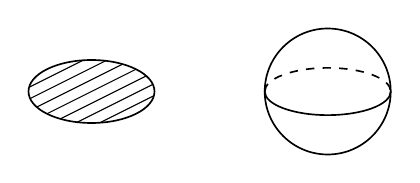
\begin{tikzpicture}[line width=.6]
    \draw (0,0) ellipse (.8 and .4);
    \begin{scope}
        \clip (0,0) ellipse (.8 and .4);
        \draw[thin] (1.7,.4) -- (.1,-.4)
                    (1.4,.4) -- (-.2,-.4)
                    (1.1,.4) -- (-.5,-.4)
                    (.8,.4) -- (-.8,-.4)
                    (.5,.4) -- (-1.1,-.4)
                    (.2,.4) -- (-1.4,-.4)
                    (-.1,.4) -- (-1.7,-.4);
    \end{scope}
    \draw (3,0) circle (.8);
    \draw[dashed] (2.2,0) arc (180:0:.8 and .3);
    \draw (2.2,0) arc (180:360:.8 and .3);
\end{tikzpicture} \]

This theorem is often proved as a consequence of
the uniformisation theorem of Riemann surfaces,
using the fact that every Riemannian $2$-manifold can be given isothermal coordinates
so that it becomes a Riemann surface.
Here we give it a new and direct proof.

\begin{proof}
By (\ref{cor:handle-decomp}) the manifold is diffeomorphic to a good $2$-handlebody $N$.
By (\ref{prop:0-handle}) we may assume it is a good weak handlebody with only one $0$-handle.
Consider the handle chain complex with $\Z_2$ coefficients
\[ \cdots\to0\to C_2(N;\Z_2)\xrightarrow{\partial_2}C_1(N;\Z_2)\xrightarrow{\partial_1}\Z_2. \]
Since $H_0(N;\Z_2)\simeq\Z_2$, we have $\partial_1=0$.
Since $N$ is simply connected, $H_1(N;\Z_2)=0$. Thus $\partial_2$ is surjective.
Note that the belt of a $1$-handle is $S^0$, i.e.\ two points.
Since $\partial_2$ is surjective,
these two points must intersect with either (a) two different $2$-handles,
or (b) only one $2$-handle in one point.
Thus we have a graph $G$,
with vertices corresponding to the $2$-handles,
and edges corresponding to $1$-handles in case (a).
For each $1$-handle in case (b), we add an ``external edge'' that connects one vertex with ``infinity''.
This can be interpreted as an infinite sequence of vertices and edges,
so that $G$ is rigorously a graph.
This graph is locally finite, and does not have \term{loops}
(i.e.\ edges whose endpoints are the same vertex).

We take a maximal tree in each connected component of $G$,
and then apply (\ref{thm-cancel-weak}) in the form of (\ref{thm:cancel-infinite}).
The effect is that these trees are collapsed.
By the same reason as above, the collapsed graph will not have loops.
Thus the resulting graph will have no edges at all.
This means that the resulting weak handlebody has no $1$-handles.
Therefore, if it has a $2$-handle, then it is the sphere;
if not, then it is the open disk.
\end{proof}

\begin{corollary}
    $\R^2$ has a unique smooth structure. \qed
\end{corollary}

This method generalises to prove the following.

\begin{theorem}\label{thm:2-mfd-noncompact}
Every connected non-compact $2$-manifold is diffeomorphic to a weak $(2,1)$-handlebody.
\end{theorem}

\begin{proof}
Similarly, the manifold is diffeomorphic to a good weak $2$-handlebody $N$
with only one $0$-handle.
We construct something like a graph, denoted $G$, in the same way,
except that edges ($1$-handles) need not have vertices ($2$-handles) as their endpoints.
We ignore those edges with no endpoints for a while,
and collapse maximal trees of connected components of the remaining part of $G$.
The resulting thing should be a collection of vertices,
each possibly with some loops attached to it,
and some isolated edges.

We need to show that there are actually no vertices.
Suppose the contrary. Then at some stage,
a first $2$-handle will be attached to a (non-weak)
$(2,1)$-handlebody with only one $0$-handle.
Since every edge is a loop, it follows that whenever the image of the attaching map
passes through a $1$-handle, it passes through both sides of it.
By an elementary argument in combinatorics, if it passes through a $1$-handle,
then it will pass through the whole boundary.
This means that there will be no boundary after this attaching,
and thus $N$ must be compact, a contradiction.
\end{proof}

Together with the following well-known result,
the preceding theorem will give a classification for
all boundaryless $2$-manifolds with finite topology.

The following result will also be proved in our handle-theoretic way.

\begin{theorem}[Classification of closed surfaces]
Every connected closed $2$-manifold is diffeomorphic to one of the following.
\begin{enum}
\item The orientable surface $\Sigma_g:=$ connected sum of $g$ tori,
where $g=0,1,\dotsc$ \emph{(where $\Sigma_0:=S^2$)}, with Euler characteristic $\chi(\Sigma_g)=2-2g$.
\item The non-orientable surface $\Pi_k:=$ connected sum of $k$ projective planes,
where $k=1,2,\dotsc$, with Euler characteristic $\chi(\Pi_k)=2-k$.
\end{enum}
\end{theorem}

\begin{proof}
Let $N$ be a good handle decomposition.
By (\ref{prop:0-handle}), we assume that $N$ has only one $0$-handle.
Taking the dual handlebody, we may assume $N$ has only one $2$-handle.
Let $k$ denote the number of $1$-handles, and we prove by induction on $k$
that the diffeomorphism type is decided by orientability and $k$.

If $k=0$, then $N\simeq S^2$. If $k=1$, an easy argument yields $N\simeq\R P^2$.
Next we suppose $k\geq2$.
If we remove the $2$-handle, we get a $(2,1)$-handlebody with boundary $S^1$.
If we remove one more $1$-handle, one of the following happens.

(i) The boundary is two circles, and the surface is orientable.
Thus the original surface is recovered by attaching a cylinder $S^1\times I$ along these circles,
and the orientability of the original surface decides how (regarding orientation) to attach this cylinder.
If we instead attach two $2$-handles along these circles,
then the Euler characteristic will increase by $2$.
By the inductive hypothesis, the resulting surface $S$ is decided by $k$.
By (\ref{prop:move-disk}) and (\ref{cor:isotopy-ext}),
if we take two disjoint disks on $S$ and remove their interiors,
then the resulting surface $S'$ is unique up to a diffeomorphism.
Thus our original surface is decided by $k$.

(ii) The boundary is two circles, and the surface is non-orientable.
This case is the same as (i) except that by (\ref{prop:move-disk}),
the two ways (regarding orientation) of attaching a cylinder result in the same surface.

(iii) The boundary is one circle.
In this case the original surface must be non-orientable,
and will be recovered by attaching a M\"obius band along the circle.
If we instead attach a $2$-handle along the circle,
then the Euler characteristic increases by $1$.
By a same argument as in (i),
it remains to show that the connected sum $\Sigma_g\mathbin\#\Pi_1$
is diffeomorphic to $\Pi_{2g}\mathbin\#\Pi_1\simeq\Pi_{2g+1}$.
This follows from the observation that $\Pi_3\simeq\Sigma_1\mathbin\#\Pi_1$.
\end{proof}

Now we may apply our results to non-compact manifolds.
We say a manifold has \term{finite topology},
if its (say $\R$-coefficient) homology groups are finite dimensional.

\begin{theorem}[Classification of $2$-manifolds]
Every connected boundaryless $2$-manifold with finite topology
is diffeomorphic to either one of the closed surfaces $\Sigma_g$ and $\Pi_k$,
or one of them with a finite number of points removed.
\end{theorem}

\begin{proof}
The compact case follows from the preceding theorem.
For the non-compact case, by (\ref{thm:2-mfd-noncompact}),
the manifold must be a weak $(2,1)$-handlebody with one $0$-handle.
By the finiteness assumption, it must have finitely many $1$-handles.
Thus it is the interior of a finite $(2,1)$-handlebody,
whose boundary is a compact $1$-manifold, i.e.\ a finite number of circles.
After attaching $2$-handles along these circles,
it would become a closed surface, whence the result follows.
\end{proof}

The remaining case to a complete classification of $2$-manifolds
is that of weak $(2,1)$-handlebodies
with one $0$-handle and infinitely many $1$-handles.
However, classifying them is very difficult,
and even the open subsets of $\R^2$ can not easily be classified.
On the other hand, we can obtain partial results.
For example, using the results in this paper, one can show that
after multiplying by $\R$,
all the orientable ones will become diffeomorphic $3$-dimensional manifolds.


\section{热核} \label{sect-7}

\subsection{广义 Laplace 算子}

我们回忆, 若 $E_1, E_2 \to M$ 是两个光滑向量丛,
则一个 $k$ 阶微分算子 $D \: \Gamma (E_1) \to \Gamma (E_2)$ 局部上具有如下形式:
\[ D (s^i e_i^{(1)}) = \sum_{ |\alpha| \leq k } 
    a_{i}^{j \alpha} \, ( \partial_{\alpha} s^i ) \, e_j^{(2)}. \]

\begin{definition}
    设 $D \: \Gamma (E_1) \to \Gamma (E_2)$ 是 $k$ 阶微分算子.
    它的\term{符号} (symbol) 定义为向量丛的映射
    \begin{align*}
        \sigma_D \: \operatorname{Sym}^k (T^* M) \otimes E_1 &\to E_2, \\
        e^\alpha \otimes e_i^{(1)} &\mapsto a_i^{j \alpha} e_j^{(2)}.
    \end{align*}
    换言之, $\sigma_D$ 的分量由 $(\sigma_D)_i^{j \alpha} = a_i^{j \alpha}$ 给出.
\end{definition}

例如, $\bbR^n$ 上的 Laplace 算子 $\Delta = -\sum_i ( \partial / \partial x^i )^2$ 的符号
\[ \sigma_{\Delta} \: \operatorname{Sym}^2 (\bbR^n) \to \bbR \]
就是 Euclid 内积的相反数.

\begin{definition}
    微分算子 $D \: \Gamma (E) \to \Gamma (E)$ 称为\term{椭圆} (elliptic) 的,
    如果对任意 $x \in M$ 以及 $0 \neq v \in T_x^* M$, 映射
    \[ \sigma_D (v, \dotsc, v) \: E_x \to E_x \]
    都是向量空间的自同构.
\end{definition}

例如, $\bbR^n$ 上的 Laplace 算子 $\Delta$ 就是椭圆微分算子,
因为 $\bbR^n$ 中非零向量和自身的内积不会等于 $0$.

\begin{definition}
    设 $M$ 是 Riemann 流形, $E \to M$ 是光滑向量丛.
    微分算子 $H \: \Gamma (E) \to \Gamma (E)$ 
    称为一个\term{广义 Laplace 算子} (generalised Laplacian), 如果
    \begin{itemize}
        \item 
            $H$ 是二阶算子.
        \item
            对任意 $x \in M$ 以及 $v, w \in T_x^* M$, 映射
            \[ \sigma_H (v, w) \: E_x \to E_x \]
            等于和 $-\langle v, w \rangle$ 的数乘.
    \end{itemize}
    等价地说, 广义 Laplace 算子在局部坐标系下表示为如下形式:
    \[ H = -g^{ij} \, \partial_i \, \partial_j + (\text{一阶微分算子}), \]
    其中 $g^{ij}$ 是 Riemann 度量.
\end{definition}

\begin{example}
    设 $M$ 是 Riemann 流形, $E \to M$ 是光滑向量丛.
    给定 $E$ 上的联络 $\nabla$, 我们就能定义对应的 Laplace 算子 $\Delta$,
    也叫做 \term{Laplace--Beltrami 算子}. 它在局部坐标系中定义为
    \[ \Delta s = -g^{ij} \, \bigl( \nabla_i \nabla_j \, s 
        - \Gamma_{ij}^k \nabla_k \, s \bigl), \]
    其中 $\nabla_i$ 是沿坐标向量场 $e_i$ 的方向导数.
    则每个联络 $\nabla$ 给出的 Laplace 算子都是广义 Laplace 算子. \varqed
\end{example}

\begin{proposition} \label{thm-7-gen-lap}
    如果 $H$ 是 $E$ 上的广义 Laplace 算子, 那么存在 $E$ 上的联络 $\nabla$, 使得
    \[ H = \Delta + f, \]
    其中 $\Delta$ 是联络 $\nabla$ 的 Laplace 算子, $f \in C^\infty (M)$.
\end{proposition}

这一结论的证明见 \cite[命题~2.5]{bgv}.


\subsection{\texorpdfstring{$\bbR^n$}{ℝⁿ} 中的热核}

在这一小节中, 我们回忆 $\bbR^n$ 中热方程的解法.

\term{热方程} (heat equation) 是偏微分方程中的一类基础的方程,
其初值问题叙述如下: 给定 $\bbR^n$ 上的函数 $f$, 求一个函数
\[ u (x, t) \quad (x \in \bbR^n , \ t \in \bbR_{\geq 0}), \]
满足
\[ \Biggl \{ \begin{array}{l}
    \partial_t u = - \Delta_x u, \\
    u |_{t=0} = f,
\end{array} \]
其中 $\Delta_x$ 表示 $\bbR^n$ 方向的 Laplace 算子.
热方程可以看作是描述了 $\bbR^n$ 中温度 $u$ 随着时间 $t$ 的演化过程.

\begin{definition}
    $\bbR^n$ 的\term{热核} (heat kernel) 是函数
    \[ k_t (x, y) = \frac {1} {(4 \uppi t)^{n/2}} \, \upe^{-|x-y|^2 / 4t}
        \quad (x, y \in \bbR^n, \ t > 0). \]
\end{definition}

热核 $k_t (x, y)$ 满足以下性质:
\[ \Biggl \{ \begin{array}{l}
    (\partial_t + \Delta_x) \, k_t (x, y) = 0, \\
    k_t (x, y) |_{t=0} = \delta (x, y),
\end{array} \]
其中 $\delta (x, y)$ 是 $\delta$ 函数. 
因此, 为了解出热方程的初值问题, 只需令
\[ u (x, t) = \int_{\bbR^n} k_t (x, y) \, f (y) \, dy, \]
就能满足
\[ \Biggl \{ \begin{array}{l}
    (\partial_t + \Delta_x) \, u = 0, \\
    u |_{t = 0} = \int_{\bbR^n} \delta (x, y) \, f (y) \, dy = f (x).
\end{array} \]
当然, 这里的推导不是完全严格的, 我们在此忽略有关的细节.

我们把由上面的卷积给出的 $u (x, t)$ 记作
\[ u = K_t (f) = \upe^{-t \Delta} f, \]
其中 $\upe^{-t \Delta}$ 是形式的记号, 在计算中能给人以直观.


\subsection{广义 Laplace 算子的热核}

下面, 设 $M$ 是紧 Riemann 流形, $E \to M$ 是光滑向量丛.

我们回忆, 在分析学中, $\bbR$ 上的一个\term{分布} (distribution)
是指一个连续线性泛函
\[ \phi \: C_{\mathrm{c}}^\infty (\bbR) \to \bbR, \]
其中左边是 $\bbR$ 上紧支光滑函数的空间, 带有 \term{$C^\infty$ 拓扑},
也就是说, 一列函数的收敛性等价于它们的支集包含于一个公共的紧集,
并且对每个 $n$, 它们的 $n$ 阶导数在这个紧集上一致收敛.

例如, 任何一个局部 $L^1$ 函数 $g \: \bbR \to \bbR$ 都可以看作 $\bbR$ 上的分布:
对 $f \in C_{\mathrm{c}}^\infty (\bbR)$, 定义
\[ g (f) = \int_{\bbR} f(x) \, g(x) \, dx, \]
就能将 $g$ 视作泛函. 再例如, $\delta$ 函数
\[ \delta (f) = f (0) \]
也是分布, 它可以看作在 $0$ 处取值 $+\infty$, 在别处取值 $0$, 但总积分为 $1$ 的函数.

分布的概念可以推广到向量丛的截面.
因为我们假设了 $M$ 是紧流形, 所以我们不再需要担心紧支的问题.

\begin{definition}
    在本节开头的假设下, $E$ 的\term{分布截面} (distributional section) 的集合定义为
    \[ \Gamma_{\mathrm{dist}} (E) = \Gamma (E^\vee) ^\vee, \]
    其中 $\Gamma (E^\vee)$ 带有 $C^\infty$ 拓扑,
    $\Gamma (E^\vee) ^\vee$ 是它的连续对偶空间.
\end{definition}

\begin{remark}
    这个定义带来了一个问题: 我们可以把普通的截面看成分布截面,
    但这个过程其实依赖于 $M$ 的度量: 若 $s$ 是普通截面, $f \in \Gamma(E^{\vee})$,
    我们需要定义
    \[ s(f) = \int_M \langle f, s \rangle \, \mathrm{vol} , \]
    其中 $\mathrm{vol}$ 是 $M$ 的体积密度
    (当 $M$ 可定向时, 它就是体积形式), 
    但这个表达式的值依赖于 $\mathrm{vol}$ 的选取.
    
    为了做到和度量无关, 我们可以将 $\Gamma_{\mathrm{dist}} (E)$ 定义为
    \[ \Gamma \bigl( E^\vee \otimes |{\wedge^n \, T^* M}| \bigr) ^\vee, \]
    其中 $n = \dim M$. 因为密度线丛 $|{\wedge^n \, T^* M}|$ 是平凡线丛,
    所以这和之前的定义是同构的, 但同构的选取和度量有关.
    为了简洁性, 我们不采用这种做法. \varqed
\end{remark}

$\bbR^n$ 中的热方程可以以 $\bbR^n$ 上的一个分布为初值.
事实上, 允许以分布作为初值是有好处的,
因为热核实际上就是以 $\delta$ 函数为初值的热方程的解.
通过同样的方法, 我们可以定义广义 Laplace 算子的热核.

\begin{definition}
    设 $E_1, E_2 \to M$ 是两个光滑向量丛. 设
    \[ K \: \Gamma_{\mathrm{dist}} (E_1) \to \Gamma (E_2) \]
    是一个连续线性映射. 那么, $K$ 的\term{核} (kernel) 是指一个截面
    \[ k \in \Gamma \bigl( M \times M, \ \Hom (p_2^* E_1, p_1^* E_2) \bigr), \]
    其中 $p_1, p_2 \: M \times M \to M$ 是投影,
    满足对任意的 $s \in \Gamma_{\mathrm{dist}} (E_1)$, 都有
    \begin{equation} \label{eq-7-kernel}
        (K s) (x) = \int_M k (x, y) \, s (y) \, dy,
    \end{equation}
    其中右边的含义是配对 $\langle s, k(x, -) \rangle$,
    这里 $k (x, -) \in \Gamma (E_1^\vee) \otimes (E_2)_x$.
\end{definition}

核的存在性是分布理论的一个重要的结论.

\begin{theorem} [Schwartz 核定理]
    沿用上面的记号, 我们有向量空间的同构
    \begin{align*}
        L \bigl( \Gamma_{\mathrm{dist}} (E_1), \ \Gamma (E_2) \bigr) \ 
            & \simeq \ \Gamma \bigl( M \times M, \ \Hom (p_2^* E_1, p_1^* E_2) \bigr), \\
        K \ & \leftrightarrow \ k,
    \end{align*} 
    其中 $L$ 表示连续线性映射的空间.
\end{theorem}

对于广义 Laplace 算子的热方程而言,
定理说明热方程的解的存在性等价于热核的存在性,
但它们的存在性需要我们稍后证明.

\begin{definition}
    设 $H \: \Gamma (E) \to \Gamma (E)$ 是广义 Laplace 算子.
    它的\term{热核} (heat kernel) 是一族截面
    \[ k_t \in \Gamma \bigl( M \times M, \ \Hom (p_2^* E, p_1^* E) \bigr)
        \quad (t > 0), \]
    关于 $t$ 有一阶导数, 并满足
    \[ \Biggl \{ \begin{array}{l}
        (\partial_t + H_x) \, k_t (x, y) = 0, \\
        k_t (x, y) |_{t=0} = \delta (x, y).
    \end{array} \]
    这里, 第二个式子的严格意义是, 对任意 $s \in \Gamma(E)$, 有一致收敛性
    \[ \lim _{t \to 0} K_t (s) = s, \]
    这里 $K_t$ 由 (\ref{eq-7-kernel}) 给出.
\end{definition}

热核的存在性将在后面证明, 但我们先叙述这一结论.

\begin{theorem} \label{thm-7-heat-ker-exists}
    每个广义 Laplace 算子都有热核.
\end{theorem}


\subsection{渐进展开}

我们先假定热核的存在性, 然后研究它在 $t \to 0$ 时的渐进行为.
我们将从中得到关于曲率的信息, 并在以后把它和示性类联系起来.

和前面一样, 我们设 $M$ 是紧 Riemann 流形, $E \to M$ 是光滑向量丛,
$H \: \Gamma (E) \to \Gamma (E)$ 是一个广义 Laplace 算子.

我们固定 $y \in M$, 然后取法坐标系
\[ x = \exp_y X. \]
我们记
\[ q_t (x, y) = \frac {1} {(4 \uppi t)^{n/2}} \, \upe^{-|X|^2 / 4t}, \]
并将 $H$ 的热核 $k_t$ 与它进行比较. 我们希望得到形如
\[ k_t = q_t \cdot \sum_{i=0}^\infty t^i \, \Phi_i \]
的表达式,
其中 $\Phi_i \in \Gamma \bigl( M \times M, \ \Hom (p_2^* E, p_1^* E) \bigr)$.
我们试着算出这些 $\Phi_i$.

我们考虑 $E$ 上由 (\ref{thm-7-gen-lap}) 给出的联络 $\nabla$.

\begin{lemma}
    设 $s_t \in \Gamma(E)$ ($t > 0$) 是一族截面, 关于 $t$ 有一阶导数. 则
    \[ (\partial_t + H) (q_t s_t) =
        q_t \, (\partial_t + t^{-1} \, \nabla_R + B) \, s_t, \]
    其中 $R = X^i e_i$ 是径向向量场, 
    微分算子 $B = \sqrt{g}{}^{1/2} \circ H \circ \sqrt{g}{}^{-1/2}$,
    其中 $\sqrt{g}$ 是 $\sqrt{\det \smash{(g_{ij})}}$ 的缩写.
\end{lemma}

\begin{proof}
    我们按 Leibniz 法则展开式子左边:
    \[ \text{左边} = (\partial_t q_t) \, s_t + q_t \, (\partial_t s_t) +
        (\Delta q_t) \, s_t + q_t \, (Hs_t) -2 \langle \nabla q_t, \nabla s_t \rangle, \]
    其中 $\Delta$ 是 $M$ 上的 Laplace 算子.
    而由热核 $q_t$ 的性质, 以及法坐标系中计算协变导数和 Laplace 算子的公式, 我们有
    \begin{align*}
        -2 \nabla q_t &= q_t \, (t^{-1} \, R + d \log \sqrt{g}), \\
        (\partial_t + \Delta) \, q_t &= \sqrt{g}{}^{1/2} \, 
            (\Delta \sqrt{g}{}^{-1/2}) \, q_t,
    \end{align*}
    故只需证
    \[ B = H + \nabla_{d \log \sqrt{g}} + 
        \sqrt{g}{}^{1/2} \, (\Delta \sqrt{g}{}^{-1/2}), \]
    直接计算即可验证这一等式.
\end{proof}

\begin{definition}
    如果给定一族截面
    \[ \Phi_i \in \Gamma \bigl( M \times M, \ \Hom (p_2^* E, p_1^* E) \bigr)
        \quad (i = 0, 1, \dotsc), \]
    使得对每个 $y \in M$, 都有
    \begin{numcases}{}
        \label{eq-7-formal-sol-1} 
        \Phi_0 (y,y) = I \qquad \in \End (E_y), \\
        \label{eq-7-formal-sol-2}
        (\partial_t + t^{-1} \, \nabla_R + B) \, 
            \sum_{i=0}^\infty t^i \, \Phi_i (-, y) = 0,
    \end{numcases}
    那么形式幂级数
    \[ k_t (x, y) = q_t (x, y) \cdot \sum_{i=0}^\infty t^i \, \Phi_i (x, y) \]
    称为热方程的一个\term{形式解} (formal solution).
\end{definition}

在引理中取 $s_t = \sum_i t^i \, \Phi_i (x, y) \, v$, 其中 $v \in E_y$,
我们看出, 如果定义中给出的 $k_t$ 确实是热核, 那么 (\ref{eq-7-formal-sol-2}) 一定成立.
事实上, 这个定义描述了热核 $k_t$ 在对角线 $M \subset M \times M$ 附近的渐进展开.

\begin{theorem}
    存在唯一的形式解. 并且, $\Phi_i$ 满足递归公式
    \[ \Phi_i (x, y) = - \int_0^1 s^{i-1} B_x \, \Phi_{i-1} (x_s, y) \, ds, \]
    其中 $B_x$ 表示 $B$ 作用于 $x$ 分量, $x_s = \exp_y (sX)$.
\end{theorem}

\begin{proof}
    实际上, (\ref{eq-7-formal-sol-2}) 等价于
    \[ \Biggl\{ \begin{array}{l}
        \nabla_R \, \Phi_0 = 0, \\
        (\nabla_R + i) \, \Phi_i = -B_x \, \Phi_{i-1}.
    \end{array} \]
    第一个式子说明, $\Phi_0 (x, y) \: E_y \to E_x$ 一定是沿径向的平行移动.
    为了从第二个式子导出递归公式, 考虑
    \[ \phi_i (s) = s^i \, \Phi_i (x_s, y). \]
    则 $\phi_i (0) = 0$, 且
    \[ \phi'_i (s) = (i s^{i-1} + s^i \nabla_{R/s}) \, \Phi_i (x_s, y) 
        = -s^{i-1} B_x \, \Phi_{i-1} (x_s, y). \qedhere \]
\end{proof}

\begin{example}
    设 $H = \Delta$ 是联络给出的 Laplace 算子. 由递归公式,
    \begin{align*}
        \Phi_1 (y, y) &= -B_x \, \Phi_0 (x, y) |_{x=y} \\
        &= - \Delta \bigl( \sqrt{g}{}^{-1/2} \, \Phi_0 (x, y) \bigr) \big|_{x=y}
            \hspace{3em} ( \text{因 $\sqrt{g} \big|_{x=y} = 1$} ) \\
        &= - \bigl( \Delta \sqrt{g}{}^{-1/2} \bigr) \, \Phi_0 (y, y)
            - \sqrt{g}{}^{-1/2} \, \cancel{\Delta \Phi_0 (x, y)} |_{x=y} \\
            & \hspace{3em} {} + 2 \bigl\langle \nabla \sqrt{g}{}^{-1/2}, 
            \cancel{\nabla \Phi_0 (x, y)} \bigr\rangle \big|_{x=y} \\
        &= \frac{1}{3} R \cdot \mathrm{id},
    \end{align*}
    其中 $R$ 是 $M$ 的标量曲率, 被划掉的部分等于 $0$, 因为对任何 $v \in E_y$,
    向量场 $\Phi_0 (x, y) \, v$ 都是平行移动得到的,
    故在 $x = y$ 处的所有协变导数都为 $0$. 最后一步是通过公式
    \[ g_{ij} = \delta_{ij} + \frac{1}{3} R_{ikjl} x^k x^l + \text{高阶项} \]
    得到的. 这个例子说明, $\Phi_1$ 蕴涵了关于流形曲率的信息. \varqed
\end{example}

我们将上面的讨论总结如下.

\begin{theorem} \label{thm-7-asymp-exp}
    在对角线 $M \subset M \times M$ 的一个邻域内,
    $H$ 的热核 $k_t$ 在 $t \to 0$ 时具有如下渐进展开式:
    \[ k_t (x, y) \sim \frac {1} {(4 \uppi t)^{n/2}} \, \upe^{-d(x, y)^2 / 4t} \cdot
        \sum_{i=0}^\infty t^i \, \Phi_i (x, y), \]
    其前 $N$ 项部分和在 $C^k$-范数下与 $k_t$ 的误差是 $O (t^{N - n/2 - k/2 + 1})$.
\end{theorem}

这里, 最后的误差估计是由下一小节的构造过程给出的.


\subsection{热核的构造}

这一小节, 我们简要概述如何证明广义 Laplace 算子的热核的存在性 (\ref{thm-7-heat-ker-exists}).

为了演示我们构造的方法, 我们先从一个简化的模型开始.
在这个简化模型中, 我们将无限维空间上的算子 $H \: \Gamma (E) \to \Gamma (E)$
换成有限维空间上的算子.

下面, 设 $V$ 是有限维向量空间, $H \in \End (V)$. 设
\[ K_t \in \End (V) \quad (t \geq 0) \]
是一族算子, 它是热方程 $(\partial_t + H) \, K_t = 0$ 的 ``近似解''.
准确地说, 它满足
\[ \Biggl\{ \begin{array}{ll}
    R_t = (\partial_t + H) \, K_t = O (t^\alpha) \quad (t \to 0), \\
    K_0 = \mathrm{id}_V,
\end{array} \]
其中 $\alpha \geq 0$ 是某个常数. 我们打算对 $K_t$ 进行调整,
从而它成为一个真正的解.

为此, 我们定义 
{\allowdisplaybreaks \begin{flalign*}
    && Q_t^0 &= K_t, & \\
    & \text{从而} &
        (\partial_t + H) \, Q_t^0 &= R_t; \\
    & \text{再定义} &
        Q_t^1 &= \int_0^t K_{t-t_1} \, R_{t_1} \, dt_1, \\
    & \text{从而} &
        (\partial_t + H) \, Q_t^1 &= R_t + \int_0^t R_{t-t_1} \, R_{t_1} \, dt_1; \\
    & \text{再定义} &
        Q_t^2 &= \int \limits _{0 \leq t_1 \leq t_2 \leq t}
        K_{t-t_2} \, R_{t_2-t_1} \, R_{t_1} \, dt_1 \, dt_2, \\
    & \text{从而} &
        (\partial_t + H) \, Q_t^2 &= R_t + \int_0^t R_{t-t_1} \, R_{t_1} \, dt_1 \\
        &&& \hspace{3em} {} + \int \limits _{0 \leq t_1 \leq t_2 \leq t} 
        R_{t-t_2} \, R_{t_2-t_1} \, R_{t_1} \, dt_1 \, dt_2,
\end{flalign*}}%
并以此类推.

\begin{proposition}
    级数 
    \[ Q_t = \sum_{k=0}^{\infty} (-1)^k Q_t^k \]
    收敛, 且给出了热方程的解. 并且,
    \[ Q_t = K_t + O(t^{1+\alpha}). \]
\end{proposition}

\begin{proof}
    对每个 $t > 0$, 存在常数 $C$, 使得对任意 $t' \leq t$, 有
    \[ |K_{t'}| < C, \quad |R_{t'}| < C. \]
    从而
    \begin{align*}
        |Q_t^k| &< C^{k+1} \int \limits _{0 \leq t_1 \leq \cdots \leq t_k \leq t}
            dt_1 \, \cdots \, dt_k \\
        &= C^{k+1} \, \frac{t^k}{k!}.
    \end{align*}
    这蕴涵了级数的收敛性. 用同样的方法, 借助上面的计算, 不难验证 $Q_t$ 是热方程的解.
\end{proof}

下面, 我们来考虑一般的情况, 即 $H \: \Gamma (E) \to \Gamma (E)$
是广义 Laplace 算子的情况.

我们注意到一个事实: 如果算子 $P, Q$ 的核分别是 $p, q$,
那么算子 $PQ$ 的核是卷积 $p * q$, 定义为
\[ (p * q)(x, y) = \int_M p(x, z) \circ q(z, y) \, dz. \]

和在简化模型中一样, 我们首先取定一个近似解 $K_t$.
对 $s \in \Gamma (E)$, 我们令
\[ (K_t s) (x) = \int_M k_t^N (x, y) \, s(y) \, dy, \]
其中 $N$ 是取定的正整数, $k_t^N$ 定义为
\[ k_t^N (x, y) = \psi(d(x,y)) \cdot 
    \bigl( \text{(\ref{thm-7-asymp-exp}) 中的部分和 $\textstyle \sum_0^N$} \bigr), \]
其中 $\psi$ 是一个光滑函数, 在 $0$ 附近取值恒为 $1$, 且 $\psi([\epsilon, +\infty)) = 0$,
其中 $\epsilon > 0$ 取得使 $k_t^N$ 在整个 $M \times M$ 上有定义.

为使记号简洁, 下面我们就记
\[ k_t = k_t^N. \]

我们和之前一样定义算子 $Q_t^k$. 它的核是
\[ q_t^k = \int \limits_{0 \leq t_1 \leq \cdots \leq t_k \leq t}
    k_{t-t_k} * r_{t_k-t_{k-1}} * \cdots * r_{t_1} \, dt_1 \, \cdots \, dt_k, \]
其中 $r_t = (\partial_t + H_x) \, k_t$ 是算子 $R_t$ 的核.

通过直接计算, 我们能给出估计
\[ \| r_t \|_{C^\ell} \leq C(\ell) \, t^{N - n/2 - \ell/2}. \]
计算过程不在这里给出, 见 \cite[定理~2.29]{bgv}.
注意到这里 $t^{N - n/2}$ 就是 $k_t^N$ 的最高次项.
由 $q_t^k$ 的卷积表达式, 我们有
\[ \| q_t^k \|_{C^\ell} \leq C(\ell) \, t^{k(N - n/2) - \ell/2} \, t^k
    \operatorname{vol} (M)^{k-1}, \]
这里 $C(\ell)$ 是和上面不同的常数; $\operatorname{vol} (M)^{k-1}$ 来自于卷积的定义.
卷积中 $k_t$ 一项没有出现在估计中, 因为算子 $K_t$ 关于 $t$ 一致有界
(参见上述引用的定理).

这一估计给出了级数 $\sum_k (-1)^k q_t^k$ 的收敛性.

\begin{theorem}
    当 $N > n/2 + 1$ 时, 级数
    \[ q_t = \sum_{k=0}^\infty (-1)^k q_t^k \]
    在 $C^2$-范数的意义下收敛.
    这个公式给出了算子 $H$ 的热核. \qed
\end{theorem}

作为推论, (\ref{thm-7-heat-ker-exists}) 和 (\ref{thm-7-asymp-exp})
都获得了证明.



\section{Dirac 算子} \label{sect-8}

Dirac 算子的理论起源于量子力学.
为了在量子力学中引入狭义相对论,
需要对波函数的 Laplace 算子开平方而得到 Hamilton 算子.
如果波函数是普通的复值函数, 那么开平方的操作是不可能做到的.
Dirac 因而提出, 波函数应该是取值于某个 $\bbC^n$ 的函数.
这个空间 $\bbC^n$ 被称为\term{旋量空间} (spinor space).
在这个框架下, Dirac 的 Hamilton 算子自然地给出了 Clifford 代数在旋量空间中的表示.


\subsection{Dirac 算子与 Clifford 代数}

在这一节中, 设 $M$ 是 $n$ 维 Riemann 流形, $E \to M$ 是光滑向量丛.

\begin{definition}
    $E$ 上的一个 \term{Dirac 算子} (Dirac operator) 是一个一阶微分算子
    $D \: \Gamma (E) \to \Gamma (E)$, 使得 $D^2$ 是广义 Laplace 算子.
\end{definition}

\begin{example} \label{eg-8-dirac-d-dstar}
    若 $E = \wedge^\bullet \, T^* M$ 是微分形式的向量丛,
    则 $d + d^*$ 是一个 Dirac 算子. 它的平方是
    \[ (d + d^*)^2 = d d^* + d^* d, \]
    称为\term{微分形式的 Laplace 算子}.
    它与 Levi-Civita 联络给出的 Laplace 算子相差一个曲率项.
    这一关系称为 Weitzenböck 恒等式, 这里就不详述了.
    
    再例如, 若 $M$ 是 Kähler 流形, $E$ 是全纯微分形式的向量丛,
    则 $\dbar + \dbar^*$ 是一个 Dirac 算子. 此时, 相应的
    Weitzenböck 恒等式被称为 Bochner--小平 (Kodaira) 恒等式. \varqed
\end{example}

下面, 设 $D$ 是 $E$ 上的一阶微分算子. 则在局部坐标系中, 它具有
\[ D = \sum_{k=1}^n a^k \partial_k + b \]
的形式, 其中 $a^k, b \in \Gamma( \End (E) )$. 从而
\[ D^2 = \frac12 (a^i a^j + a^j a^i) \, \partial_i \partial_j + (\text{一阶算子}), \]
其中系数 $1/2$ 是因为 $\partial_i \partial_j$ 和 $\partial_j \partial_i$
在求和时被重复计算了. 因此, $D$ 是 Dirac 算子等价于
\[ a^i a^j + a^j a^i = -2 g^{ij}. \]
这个关系启发了 Clifford 代数的定义.

\begin{definition}
    设 $V$ 是 $n$ 维实向量空间, $Q$ 是 $V$ 上的二次型, 等同地看作对称双线性型.
    \term{Clifford 代数}定义为商代数
    \[ \Cl (V, Q) = \frac {T(V)} {v \cdot w + w \cdot v = -2 Q(v, w)}, \]
    其中 $T(V) = \bigoplus_{k \geq 0} V^{\otimes k}$ 是 $V$ 上的张量代数.
    
    如果 $Q$ 非退化, 其标准型中有 $p$ 个正项和 $q$ 个负项, 我们就记 
    \[ \Cl_{p,q} (V) = \Cl (V, Q). \]
    我们记 $\Cl (V) = \Cl_{n,0} (V)$.
\end{definition}

不难看出, $\Cl (V, Q)$ 的维数是 $2^n$, 它的一组基是
\[ \{ e_{i_1} \cdots e_{i_k} \mid i_1 < \cdots < i_k \}, \]
其中 $\{ e_i \}$ 是 $V$ 的一组基.

\begin{example}
    我们有 $\Cl (\bbR^2) \simeq \bbH$.
    事实上, 记 $\upi, \upj$ 为 $\bbR^2$ 的标准正交基, 
    则 Clifford 代数的定义给出的关系是
    \[ \upi^2 = \upj^2 = -1, \quad \upi \, \upj + \upj \, \upi = 0. \varqedhere \]
\end{example}

由于张量代数的 $\bbZ$-分次在 $\Cl (V, Q)$ 中得到保留,
后者也是 $\bbZ$-分次代数. 特别地, 我们有:

\begin{proposition}
    Clifford 代数是超代数. \qed
\end{proposition}

\begin{definition}
    一个 \term{Clifford 模}是指 Clifford 代数 $\Cl (V, Q)$ 在一个超向量空间 $E$ 中的表示.
    也就是说, 我们有 (保持 $\bbZ_2$-分次的) 超代数同态
    \[ \Cl (V, Q) \to \End (E). \]
\end{definition}

\begin{example} \label{eg-8-symbol-map}
    超向量空间 $\wedge^\bullet \, V$ 具有自然的 $\Cl (V, Q)$-模的结构, 定义为
    \[ v \cdot \alpha = v \wedge \alpha - Q (v, -) \contr \alpha \quad
        (v \in V, \ \alpha \in \wedge^\bullet \, V), \]
    其中 $\contr$ 表示缩并. 
    若取 $V$ 关于 $Q$ 的一组正交基 $\{ e_1, \dotsc, e_n \}$,
    则上式可以写成
    \[ e_i \cdot (e_{i_1} \wedge \cdots \wedge e_{i_k}) = \Biggl\{
        \begin{array}{ll}
            e_i \wedge e_{i_1} \wedge \cdots \wedge e_{i_k}, & i \notin \{ i_1, \dotsc, i_k \}, \\
            -Q(e_i) \, e_{i_2} \wedge \cdots \wedge e_{i_k}, & i = i_1.
        \end{array} \]
    映射
    \[ \sigma \: \Cl (V, Q) \overset{\cdot 1}{\longrightarrow} \wedge^\bullet \, V \]
    是超向量空间的同构, 称为\term{符号映射} (symbol map). \varqed
\end{example}


\subsection{旋量群}

旋量群 $\Spin (n)$ 的一个著名的性质是,
它是 $\SO (n)$ 的双重覆叠 (在 $n \geq 3$ 时是万有覆叠).
也就是说, 我们有 Lie 群的正合列
\[ 0 \to \bbZ_2 \to \Spin (n) \to \SO (n) \to 0. \]
通过 Clifford 代数, 我们可以得到旋量群的一个具体的构造.

\begin{definition}
    设 $V$ 是 $n$ 维欧氏空间. 我们定义 Lie 代数
    \[ \spin (V) = \Cl (V)_2 \]
    为 Clifford 代数中分次为 $2$ 的部分, 其 Lie 括号就是 Clifford 代数中的交换子.
\end{definition}

换言之, 如果 $e_1, \dotsc, e_n$ 是 $V$ 的一组标准正交基, 那么
\[ \spin (V) = \operatorname{span} {} \{ e_i e_j \mid i \neq j \}, \]
这里, 注意到我们有反交换关系 
\[ e_i e_j = -e_j e_i. \]

\begin{proposition} \label{thm-8-spin-alg-action}
    Lie 代数 $\spin (V)$ 可以作用在 $V \subset \Cl (V)$ 上,
    作用的方式是 $a \cdot v = [a, v]$. 这个作用诱导了 Lie 代数同构
    \[ \spin (V) \simeq \so (V). \]
\end{proposition}

\begin{proof}
    首先, 我们说明对应的映射 $\phi \: \spin (V) \to \gl (V)$ 的像落在 $\so (V)$ 中.
    取 $V$ 的标准正交基 $e_1, \dotsc, e_n$. 则元素 $e_i e_j \in \spin (V)$ 的作用是
    \[ \left \{ \begin{array}{l}
        e_i \mapsto 2e_j, \\
        e_j \mapsto -2e_i, \\
        e_k \mapsto 0 \qquad (k \neq i, j).
    \end{array} \right . \]
    这一线性映射的矩阵是反对称矩阵. 这也说明 $\phi$ 是单射.
    但 $\dim \spin (V) = \dim {\wedge^2 \, V} = \dim \so (V)$,
    从而 $\phi$ 是到 $\so (V)$ 的同构.
\end{proof}

\begin{definition}
    $V$ 的\term{旋量群} (spin group) 定义为
    \[ \Spin (V) = \exp \bigl( \spin (V) \bigr), \]
    其中 $\exp$ 是指在 $\Cl (V)$ 中的幂级数.
\end{definition}

事实上, Lie 理论告诉我们,
$\Spin (V)$ 是一个以 $\spin (V)$ 为 Lie 代数的连通 Lie 群,
它是 $\Cl (V)$ 的偶数阶元素的乘法群的 Lie 子群.

\begin{example}
    设 $\{ e_i \}$ 是 $V$ 的标准正交基. 则 $i \neq j$ 时, $(e_i e_j)^2 = -1$. 因此
    \[ \exp ( t e_i e_j ) = \sum _{k=0} ^\infty \frac {t^k} {k!} \, (e_i e_j)^k
        = \cos t + (\sin t) \, e_i e_j \quad (t \in \bbR). \]
    特别地, 当 $\dim V = 2$ 时, 我们得到了圆圈群
    \[ \Spin (2) \simeq S^1. \]
    当 $\dim V = 3$ 时, 我们可以将 $\Cl (V)$ 的子代数
    $\operatorname{span} \, \{ 1, e_1 e_2, e_2 e_3, e_3 e_1 \}$ 和 $\bbH$ 等同起来.
    此时, 旋量群就是单位四元数的乘法群:
    \[ \Spin (3) \simeq S^3 \subset \bbH, \]
    因为指数映射会把虚四元数映到单位四元数. \varqed
\end{example}

\begin{proposition}
    当 $\dim V \geq 2$ 时, $\Spin (V)$ 是 $\SO (V)$ 的双重覆叠.
\end{proposition}

\begin{proof}
    考虑 $\Spin (V)$ 在 $V$ 上的作用:
    \[ g \cdot v = g v g^{-1} \quad (g \in \Spin (V), \ v \in V). \]
    我们说明, 这个作用诱导了到 $\SO (V)$ 的双重覆叠.
    
    首先, 这个 Lie 群表示对应的 Lie 代数表示就是 (\ref{thm-8-spin-alg-action}) 给出的同构.
    因此, 对应的映射 $\Spin (V) \to \SO (V)$ 是覆叠映射.
    因为元素 $-1 \in \Spin (V)$ 的作用是平凡的, 所以这个覆叠至少是二重的.
    但 $\dim V \geq 3$ 时, $\SO (V)$ 的基本群是 $\bbZ_2$, 所以这个覆叠至多是二重的;
    $\dim V = 2$ 的情况可以直接计算而得出.
\end{proof}

当 $\dim V = 1$ 时, 为了和上述结论保持一致, 我们可以重新定义
\[ \Spin (1) = \Spin (V) = \{ \pm 1 \} \subset \Cl (V). \]


\subsection{旋量}

\term{旋量} (spinor) 的名字是仿照向量 (vector) 的名字而造出来的.
这样命名的原因是, 旋量和向量有类似的性质, 它们的区别在于,
向量的旋转是在 $\SO (n)$ 中完成的, 而旋量的旋转是在 $\Spin (n)$ 中完成的,
因此, 旋量有时需要转两圈, 才能回到原来的位置.

例如, 手的角度 (旋转位置) 可以由一个单位旋量描述.
伸出右手, 掌心向上, 然后将手掌逆时针旋转一周.
这时, 手臂会处于一个不自然的位置.
接下来, 将手举过头顶, 不改变手的朝向.
这样, 手掌可以继续逆时针旋转一周 (从下向上看是顺时针),
然后恢复到正常的位置.
这一过程说明, 手需要旋转两周才能回到原来的位置.

事实上, 在三维空间中, 旋量构成的空间就是 $\bbH$,
而旋量群 $\Spin (3)$ 是单位四元数的乘法群, 它通过乘法作用在旋量空间上.

一般地说, \term{旋量空间} (spinor space), 即所有旋量构成的空间,
是旋量群 $\Spin (n)$ 的一个表示, 并且, 这个表示无法通过 $\SO (n)$ 的表示得到.

\begin{theorem} \label{thm-8-def-spinor}
    设 $V$ 是 $n$ 维欧氏空间.
    \begin{itemize}
        \item
            若 $n$ 为偶数, 则存在一个 $2^{n/2}$ 维复 Clifford 模 $S$, 使得
            \[ \Cl (V) \otimes \bbC \simeq \End (S), \]
            这个同构与二者在 $S$ 上的作用相容.
            并且, $\dim S^+ = \dim S^- = 2^{n/2-1}$.
        \item 
            若 $n$ 为奇数, 则存在一个 $2^{(n-1)/2}$ 维复 Clifford 模 $S$,
            它不带有 $\bbZ_2$-分次, 使得作为普通 (非 $\bbZ_2$-分次) 的代数, 有
            \[ \Cl (V) \otimes \bbC \simeq \End (S) \oplus \End (S), \]
            这个同构与二者在 $S$ 上的作用相容.
    \end{itemize}
    在两种情况下, 超向量空间 $S$ 称为\term{旋量空间} (spinor space).
\end{theorem}

在证明定理之前, 我们先给出这一结果的一些推论.

我们知道, 矩阵代数 $\End (S)$ 是单代数,
它唯一的不可约表示就是它在 $S$ 上的作用. 因此, 定理蕴涵了以下结论.

\begin{corollary}
    若 $n$ 为偶数, 则 $\Cl (V)$ 的所有复表示都具有
    \[ W \otimes S \]
    的形式, 其中 $W$ 是超向量空间, 带有平凡的 Clifford 作用. \qed
\end{corollary}

因为旋量群 $\Spin (V)$ 是 Clifford 代数的乘法子群,
所以, 定理也蕴涵了关于旋量群的表示的结论.

\begin{corollary}
    旋量空间 $S$ 是旋量群 $\Spin (V)$ 的一个表示.
    当 $n$ 为偶数时, 它分裂成旋量群的两个不可约表示
    \[ S = S^+ \oplus S^-. \]
    当 $n$ 为奇数时, $S$ 本身就是不可约的.
\end{corollary}

\begin{proof}
    记 $\Cl^+ (V) \subset \Cl (V)$ 为偶数阶元素构成的子代数, 
    则 $\Spin (V) \subset \Cl^+ (V)$.
    因为 $\Spin (V)$ 包含 $\Cl^+ (V)$ 作为向量空间的一组基,
    所以 $\Cl^+ (V)$ 的不可约表示一定诱导 $\Spin (V)$ 的不可约表示.
    
    当 $n$ 为偶数时,
    \[ \Cl^+ (V) \otimes \bbC \simeq \End^+ (S) \simeq \End (S^+) \oplus \End (S^-), \]
    从而 $S$ 分裂为 $\Cl^+ (V)$ 的两个不可约表示, 即 $S^+$ 和 $S^-$.
    
    当 $n$ 为奇数时, 定理的证明 (在下方) 表明
    \[ \Cl^+ (V) \otimes \bbC \simeq \End (S). \qedhere \]
\end{proof}

\begin{proof} [定理 \ref{thm-8-def-spinor} 的证明]
    取 $V$ 的标准正交基 $e_1, \dotsc, e_n$.
    
    若 $n$ 是偶数, 我们令
    \begin{align*}
        P &= \operatorname{span}
            ( e_1 - \upi e_2, \ e_3 - \upi e_4, \dotsc, e_{n-1} - \upi e_n ), \\
        S &= \wedge^\bullet \, P.
    \end{align*}
    则 $V \otimes \bbC = P \oplus \oline2P$.
    我们定义 $\Cl (V) \otimes \bbC$ 在 $S$ 上的作用如下:
    对 $v \in V \otimes \bbC$, $s \in S$, 定义
    \[ v \cdot s = \Biggl\{ \begin{array}{ll}
        \sqrt2 \ v \wedge s, & v \in P, \\
        -\sqrt2 \ Q(v, -) \contr s, & v \in \oline2P,
    \end{array} \]
    其中记号的意义同 (\ref{eg-8-symbol-map}).
    因为 $\dim \Cl (V) = 2^n = (\dim S)^2$, 并且,
    通过计算可以验证, $\Cl (V)$ 非零元素的作用都非零.
    因此, 这个作用诱导了同构
    \[ \Cl (V) \otimes \bbC \simeq \End (S). \]
    
    若 $n$ 是奇数, 记 $W = \operatorname{span} (e_1, \dotsc, e_{n-1})$. 
    我们有 (非 $\bbZ_2$-分次的) 同构
    \begin{align*}
        ( \Cl (W) \oplus \Cl (W) ) \otimes \bbC 
            &\simeq \Cl (V) \otimes \bbC, \\
        ( e_{i_1} \cdots e_{i_k} , \ 0 )
            &\mapsto \frac12 \bigl( e_{i_1} \cdots e_{i_k}
            + (-1)^\sigma \, \upi^{(n+1)/2} \, e_{j_1} \cdots e_{j_{n-k}} \bigr), \\
        ( 0 , \ e_{i_1} \cdots e_{i_k} )
            &\mapsto \frac12 \bigl( e_{i_1} \cdots e_{i_k}
            - (-1)^\sigma \, \upi^{(n+1)/2} \, e_{j_1} \cdots e_{j_{n-k}} \bigr),
    \end{align*}
    其中 $j_1, \dotsc, j_{n-k}$ 表示 $1, \dotsc, n$ 中除了 $i_1, \dotsc, i_k$ 外的指标,
    $\sigma$ 是 $1, \dotsc, n$ 的排列 $i_1, \dotsc, i_k, j_1, \dotsc, j_{n-k}$ 的奇偶性.
\end{proof}


\subsection{流形上的 Clifford 模}

为了将 Clifford 代数的理论应用到 Dirac 算子上,
我们需要在流形上考虑余切空间的 Clifford 代数, 它们构成一个向量丛.

\begin{definition}
    设 $M$ 是流形. $M$ 上的 \term{Clifford 丛} 
    \[ \Cl(M) \to M \]
    是在点 $x \in M$ 处的纤维为 $\Cl (T_x^* M)$
    的代数丛. $M$ 上的一个 \term{Clifford 模}是一个超向量丛
    \[ E \to M, \]
    带有 Clifford 丛的作用.
\end{definition}

为了将上一小节的理论应用到这一情形,
我们还需要将旋量空间也变成 $M$ 上的向量丛.
这需要 $M$ 具有一个\term{旋量结构}.

\begin{definition}
    设 $E \to M$ 是秩为 $n$ 的可定向光滑实向量丛.
    $E$ 的一个\term{旋量结构} (spin structure)
    是一个 $\Spin (n)$-主丛
    \[ \Spin (E) \to M, \]
    使得它对应的 $\SO (n)$-主丛与 $E$ 对应的 $\SO (n)$-主丛同构.
    
    流形 $M$ 的一个\term{旋量结构}是指余切丛 $T^* M$ 上的旋量结构.
    带有一个旋量结构的流形称为\term{旋量流形} (spin manifold).
\end{definition}

旋量结构的存在性可以通过示性类来判断.

\begin{theorem}
    设 $E \to M$ 是秩为 $n$ 的可定向光滑实向量丛.
    则 $E$ 上存在旋量结构, 当且仅当其第二 Stiefel--Whitney 类消失, 即
    \[ w_2 (E) = 0. \]
\end{theorem}

这一结论的证明可参见 \cite[定理 II.1.7]{lawson-michelsohn}.

\begin{definition}
    设 $M$ 是旋量流形. 则 $M$ 上的\term{旋量丛} (spinor bundle)
    \[ S(M) \to M \]
    是一个复向量丛, 其纤维是由 $M$ 的旋量结构给出的旋量空间.
\end{definition}

具体地说, 这一定义是这样完成的:
$\Spin (n)$-主丛的转移映射是到 $\Spin (n)$ 的映射,
而 $\Spin (n)$ 可以映到 $\End (S)$, 给出旋量丛的转移映射.

当 $\dim M$ 是偶数时, 旋量丛是一个超向量丛 $S^+ (M) \oplus S^- (M)$,
也是 $M$ 上的 Clifford 模. 由前几个小节的讨论, 我们得到下面的结论.

\begin{proposition} \label{thm-8-cl-mod-can-form}
    设 $M$ 是偶数维旋量流形. 则 $M$ 上的每个复 Clifford 模都具有
    \[ W \otimes S(M) \]
    的形式, 其中 $W$ 是超向量丛, 带有 Clifford 丛的平凡作用.
\end{proposition}

\begin{proof}
    我们只指出下面的事实: 如果 $E \simeq W \otimes S$ 是 Clifford 代数 $\Cl (V)$ 上的模,
    那么 $W \simeq \Hom_{\Cl (V)} (S, E)$.
\end{proof}


\subsection{Dirac 算子与 Clifford 超联络}

现在, 我们可以让 Dirac 算子回到我们的视野了.

\begin{definition}
    设 $E \to M$ 是光滑的超向量丛. $E$ 上的 \term{Dirac 算子}的定义和之前一样,
    但我们额外要求 $D$ 是\term{奇算子}, 它把 $E^\pm$ 的截面分别变成 $E^\mp$ 的截面.
\end{definition}

设 $D \: \Gamma (E) \to \Gamma (E)$ 是 Dirac 算子. 则局部坐标下, $D$ 具有如下形式:
\[ D = \sum_k a^k \partial_k + b, \]
其中系数 $a^k \in \Gamma (\End^- (E))$ 满足 Clifford 代数的关系.
因此, Clifford 丛 $\Cl (M)$ 可以通过这些 $a^k$ 作用在 $E$ 上,
这赋予了 $E$ 一个 Clifford 模的结构.

反过来, 在每个 Clifford 模上, 我们可以构造出相应的 Dirac 算子,
但常数项 $b$ 可以随意改变. 因此, 这些 Dirac 算子构成一个 $\Gamma (\End^- (E))$-齐性空间.

下面, 我们打算把一个 Clifford 模上的 Dirac 算子与 Clifford 超联络对应起来.

\begin{definition}
    Clifford 模 $E$ 上的 \term{Clifford 超联络}是指一个超联络 $\nabla^E$,
    满足如下的 Leibniz 法则: 若
    $a \in \Gamma ( \Cl (M) )$,\ $X \in \Gamma ( TM ),$\ $s \in \Gamma (E)$, 则
    \[ \nabla^E_X (a \cdot s) = (\nabla_X a) \cdot s + (-1)^{|a|} \, a \cdot \nabla^E_X s, \]
    其中 $\nabla$ 是 Levi-Civita 联络. 这个关系可以更简洁地写成
    \[ [ \nabla^E, \ a \cdot {} ] = \nabla a \cdot {} \ . \]
\end{definition}

\begin{proposition} \label{thm-8-nabla-s}
    设 $M$ 是偶数维旋量流形. 则 Levi-Civita 联络诱导了旋量丛
    $S = S(M)$ 上的 Clifford 超联络 $\nabla^S$.
\end{proposition}
    
\begin{proof}
    $\nabla^S$ 的构造如下: 标架丛 $\SO (T^* M)$ 上的 Levi-Civita
    联络诱导了主丛 $\Spin (M)$ 上的联络, 而由旋量丛 $S$ 的构造,
    这个联络诱导了 $S$ 上的联络 $\nabla^S$.
    
    为了验证 $\nabla^S$ 是 Clifford 超联络,
    只需验证它诱导的 $\End (S)$ 上的联络与 Clifford 丛的 Levi-Civita 联络相同.
    
    我们知道, $\Spin (n) \subset \Cl^+ (n)$ 包含了后者的一组基. 定义
    \[ \mathrm{Pin} (n) = \{ 1, e_1 \} \cdot \Spin (n) \subset \Cl (n), \]
    则 $\mathrm{Pin} (n)$ 包含 $\Cl (N)$ 的一组基.
    事实上, Lie 群 $\mathrm{Pin} (n)$ 有两个连通分支,
    其单位元所在的分支就是 $\Spin (n)$, 另一个分支包含于 $\Cl^- (n)$.
    主丛 $\Spin (M)$ 诱导了 $\mathrm{Pin} (n)$-主丛 $\mathrm{Pin} (M)$,
    它的联络就同时诱导了 $\End (S)$ 的联络和 Clifford 丛的联络.
\end{proof}

事实上, 超联络 $\nabla^S$ 在以下意义上是最本质的 Clifford 超联络.

\begin{proposition} \label{thm-8-cliff-conn}
    设 $M$ 是偶数维旋量流形, $W \to M$ 是复超向量丛. 则有一一对应
    \begin{align*}
        \{ \text{$W$ 上的超联络} \} &\leftrightarrow
            \{ \text{$W \otimes S$ 上的 Clifford 超联络} \}, \\
        \nabla^W &\leftrightarrow \nabla^W \otimes 1 + 1 \otimes \nabla^S.
    \end{align*}
\end{proposition}

\begin{proof}
    留给读者.
\end{proof}

下面, 我们构造 Clifford 超联络所对应的 Dirac 算子.

设 $M$ 是偶数维旋量流形, $E \to M$ 是 Clifford 模,
带有 Clifford 超联络 $\nabla$. 则在局部坐标下, 
这个联络作用在 $E$ 的截面上时具有如下形式:
\[ \nabla = \sum_{i=1}^n dx^i \otimes \partial_i
    + \sum_{\alpha} dx^\alpha \otimes b_\alpha, \]
其中 $\alpha$ 是 $M$ 方向的多重指标
(我们不妨只考虑递增排列、无重复的多重指标),
$b_\alpha$ 是 $\End (E)$ 的截面, 其奇偶性与 $|\alpha|$ 相反.
这里, 联络的一阶导数项是 $dx^i \otimes \partial_i$, 因为任何联络都满足这一点.

我们对应地定义 Dirac 算子
\[ D_{\nabla} = \sum_{i=1}^n (dx^i \cdot {}) \circ \partial_i
    + \sum_{\alpha} (dx^\alpha \cdot {}) \circ b_\alpha, \]
这里 $\cdot$ 表示 Clifford 作用,
例如 $dx^i$ 的作用就是我们之前的记号 $a^i$.

这一定义可以写成坐标无关的形式:

\begin{definition}
    设 $M$ 是偶数维旋量流形, $E \to M$ 是 Clifford 模,
    带有 Clifford 超联络 $\nabla$. 则 Dirac 算子 $D_{\nabla}$ 定义为
    \[ D_{\nabla} \: \Gamma (E)
        \overset{\nabla}{\longrightarrow} \Omega^\bullet (M, E)
        \simeq \Gamma (\wedge^\bullet \, T^* M \otimes E)
        \overset{\sigma^{-1}}{ \underset{\simeq}{\longrightarrow} }
            \Gamma (\Cl (M) \otimes E)
        \overset{\text{作用}}{\longrightarrow} \Gamma (E), \]
    其中 $\sigma$ 是 (\ref{eg-8-symbol-map}) 中的符号映射.
\end{definition}

\begin{theorem} \label{thm-8-dirac-cliff-conn}
    设 $M$ 是偶数维旋量流形, $E \to M$ 是复 Clifford 模.
    则上述对应关系是一一对应:
    \begin{align*}
        \{ \text{$E$ 上的 Clifford 超联络} \} &\leftrightarrow
            \{ \text{$E$ 上的 Dirac 算子} \}, \\
        \nabla &\leftrightarrow D_{\nabla}.
    \end{align*}
    这里, 我们当然要求 Dirac 算子是与 $E$ 的 Clifford 模结构相容的.
\end{theorem}

\begin{proof}
    我们已经给出了从左边集合到右边集合的映射.
    我们还需要证明这个映射是双射.
    
    我们回忆, 右边的集合是 $\Gamma (\End^- (E))$-齐性空间.
    而 (\ref{thm-8-cl-mod-can-form}) 说明
    $E$ 一定能写成 $E \simeq W \otimes S$ 的形式,
    因此, 有超向量丛的同构
    \[ \End (E) \simeq \End (S) \otimes \End (W)
        \simeq \Cl (M) \otimes \End_{\Cl (M)} (E), \]
    其中 $\End_{\Cl (M)} (E)$ 表示 $E$ 作为 Clifford 模的自同态,
    不要求保持 $\bbZ_2$-分次. 从而, 我们有同构
    \begin{multline*}
        \Gamma (\End^- (E))
        \simeq \Gamma^- \bigl( \Cl (M) \otimes \End_{\Cl (M)} (E) \bigr) \\
        \overset{\sigma}{ \underset{\simeq}{\longrightarrow} }
            \Gamma^- \bigl( \wedge^\bullet \, T^* M \otimes \End_{\Cl (M)} (E) \bigr)
        \simeq \Omega^- \bigl( M, \End_{\Cl (M)} (E) \bigr).
    \end{multline*}
    如果这个映射将截面 $s$ 映到形式 $\omega$, 那么
    \[ D_{\nabla} + s = D_{\nabla + \omega}. \]
    因此, 我们只需要验证, $\nabla + \omega$ 是 Clifford 超联络当且仅当
    \[ \omega \in \Omega^- \bigl( M, \End_{\Cl (M)} (E) \bigr). \]
    我们将这一验证留给读者.
\end{proof}



\section{指标定理 (上)} \label{sect-9}

在这一节中, 我们将前两节的内容整合起来, 证明 Atiyah--Singer 指标定理.


\subsection{Dirac 算子的指标}

在这一小节中, 设 $M$ 是紧 Riemann 流形,
$E \to M$ 是带有 Riemann 或 Hermite 度量的超向量丛
(我们要求 $E^+ \perp E^-$), 并考虑 $E$ 上的\term{自伴随} Dirac 算子 $D$.
也就是说, 我们有
\[ D = \biggl( \, \begin{matrix}
    0 & D^- \\ D^+ & 0
\end{matrix} \, \biggr), \quad D^- = (D^+)^*, \]
其中 $D^{\pm} \: E^{\pm} \to E^{\mp}$.
例如, (\ref{eg-8-dirac-d-dstar}) 给出的例子 $d + d^*$ 和 $\dbar + \dbar^*$
都是自伴随 Dirac 算子.

\begin{definition}
    自伴随 Dirac 算子 $D$ 的\term{指标} (index) 是
    \begin{align*}
        \ind (D) &= \dims \ker D \\
        &= \dim \ker D^+ - \dim \ker D^- \\
        &= \dim \ker D^+ - \dim \coker D^+.
    \end{align*}
\end{definition}

$D$ 的指标是有限的, 因为
\[ D^2 = D^+ D^- + D^- D^+ \]
是广义 Laplace 算子, 它是二阶椭圆算子,
而分析学告诉我们如下事实:

\begin{fact}
    算子 $D^2$ 定义了 Hilbert 空间 $\Gamma_{L^2} (E)$ 上的一个无界算子.
    它将整个空间分成无限个特征子空间的 Hilbert 直和,
    每个特征子空间都是有限维的, 且由光滑截面构成.
    特别地, 它的核是有限维的.
    通过特征子空间分解, 我们能定义算子
    \[ K_t = \upe^{-t D^2}. \]
    它是一个\term{迹类算子} (trace-class operator),
    也就是说, 它的迹是有限的. 特别地, 它是紧算子.
\end{fact}

定理的证明可参见 \cite[定理~III.3.8]{lawson-michelsohn}.
这里的 $K_t$ 与 \S\ref{sect-7} 中一样, 给出了热方程初值问题的解.

我们取 $\Gamma_{L^2} (E)$ 的标准正交基 $\{ e_i \}_{i=1}^\infty$, 使得
\[ D^2 e_i = \lambda_i \, e_i, \quad \text{从而} \quad 
    \upe^{-t D^2} \, e_i = \upe^{-t \lambda_i} \, e_i. \]
则每个 $e_i$ 都是光滑截面. 不难算出, 算子 $D^2$ 的热核是
\begin{equation} \label{eq-9-heat-ker}
    k_t (x, y) = \sum_i \upe^{-t \lambda_i} \, e_i (x) \otimes e_i^* (y),
\end{equation}
这里 $e_i^*$ 是 $E^\vee$ 的截面,
它等于 $e_i$ 的对偶基乘以 $\mathrm{vol}(M)^{-1}$,
从而它与 $e_i$ 的配对的积分等于 $1$.

\begin{theorem} [McKean--Singer] \label{thm-9-mckean-singer}
    设 $k_t$ 是算子 $D^2$ 的热核. 则对任意 $t > 0$, 都有
    \[ \ind (D) = \trs \upe^{-t D^2} = \int_M \trs k_t (x, x) \, dx. \]
\end{theorem}

\begin{proof}
    注意到 $D^2$ 是偶算子, 即它分别作用在两个空间 $V^{\pm} = \Gamma_{L^2} (E^{\pm})$ 上.
    
    记 $V_\lambda^{\pm} \subset V^{\pm}$ 是 $D^2$ 的 $\lambda$-特征子空间.
    则复合映射
    \[ V_\lambda^+ \overset{D^+}{\longrightarrow}
        V_\lambda^- \overset{D^-}{\longrightarrow} V_\lambda^+ \]
    是乘以 $\lambda$. 因此, 当 $\lambda \neq 0$ 时,
    $V_\lambda^+ \simeq V_\lambda^-$, 从而
    \[ \trs {} \bigl( \upe^{-t D^2} |_{V_\lambda} \bigr)
        = \upe^{-t \lambda^2} \dims V_\lambda = 0. \]
    这就说明
    \[ \trs \upe^{-t D^2} = \trs {} \bigl( \upe^{-t D^2} |_{\ker D} \bigr )
        = \dims \ker D = \ind (D), \]
    这就证明了第一个等号.
    
    第二个等号是因为, 由热核的表达式 (\ref{eq-9-heat-ker}), 有
    \begin{align*}
        \trs \upe^{-t D^2}
        &= \sum_i \pm \upe^{-t \lambda_i} \\
        &= \sum_i \int_M \upe^{-t \lambda_i} 
            \trs \bigl( e_i (x) \otimes e_i^\vee (x) \bigr) \, dx \\
        &= \int_M \trs k_t (x, x) \, dx. \qedhere
    \end{align*}
\end{proof}

也就是说, Dirac 算子的指标等于热核的迹.
我们将在表达式中令 $t \to 0$, 这样, \S\ref{sect-7} 中所做的渐进展开就能派上用场.


\subsection{Atiyah--Singer 指标定理}

我们回到上一节的设定.
设 $M$ 是偶数维紧旋量流形, $E \to M$ 是复 Clifford 模.
定义 $W = \Hom_{\Cl (M)} (S, E)$, 从而
\[ E \simeq S \otimes W. \]
设 $D$ 是 $E$ 上的 Dirac 算子, 
它对应的 Clifford 超联络 (\ref{thm-8-dirac-cliff-conn}) 记为 $\nabla^E$.
由 (\ref{thm-8-cliff-conn}), 可以将 $\nabla^E$ 写成
\[ \nabla^E = \nabla^S + \nabla^W \]
的形式, 其中 $\nabla^S, \nabla^W$ 分别是 $S$ 和 $W$ 上的联络. 则 $\nabla^E$ 的曲率是
\begin{equation} \label{eq-9-curv-sum}
    \Omega^E = (\nabla^S + \nabla^W)^2 = \Omega^S + \Omega^W,
\end{equation}
这是因为在 $S \otimes W$ 上,
$\nabla^S \nabla^W + \nabla^W \nabla^S = [\nabla^S, \nabla^W] = 0$.

我们考虑算子 $D^2$ 的热核 $k_t$ 在对角线上的幂级数展开
\[ k_t (x, x) \sim \frac {1} {(4 \uppi t)^{n/2}} \sum_{i=0}^\infty t^i k_i (x), \]
其中 $k_i \in \Gamma (\End (E))$. 我们回忆上一节定义的同构
\begin{multline*}
    \Gamma (\End (E))
    \simeq \Gamma \bigl( \End (S) \otimes \End (W) \bigr)
    \simeq \Gamma \bigl( \Cl (M) \otimes \End_{\Cl (M)} (E) \bigr) \\
    \overset{\sigma}{ \underset{\simeq}{\longrightarrow} }
        \Gamma \bigl( \wedge^\bullet \, T^* M \otimes \End_{\Cl (M)} (E) \bigr)
    \simeq \Omega^\bullet \bigl( M, \End_{\Cl (M)} (E) \bigr),
\end{multline*}
其中 $\sigma$ 是 (\ref{eg-8-symbol-map}) 中的映射.
因此, 我们得到相应的微分形式
\[ \sigma (k_i) \in \Omega^\bullet \bigl( M, \End_{\Cl (M)} (E) \bigr). \]

\begin{theorem} \label{thm-9-ahat-ch}
    沿用上面的记号, 假设 $\nabla^W$ 是普通的联络.
    则微分形式 $\sigma (k_i)$ 的最高次数是 $2i$,
    且其 $2i$ 次的部分与 
    \[ \Ahat (M) \, \upe^{-\Omega^W} \]
    的 $2i$ 次部分相同, 其中 $\Ahat (M)$ 称为 \term{$\Ahat$ 类} ($\Ahat$-genus),
    定义为
    \[ \Ahat (M) = \det^{1/2} \frac {\Omega/2} {\sinh \Omega/2}, \]
    这里 $\det^{1/2} (-)$ 的意义是形式幂级数
    $\exp \tr \bigl( 2^{-1} \log (-) \bigr)$.
\end{theorem}

这个定理将在下一节证明, 其证明方法就是利用 \S\ref{sect-7} 中的 $\Phi_i$ 进行计算.

利用这个公式计算 $\ind (D)$, 就能得到指标定理.
事实上, 由 (\ref{thm-9-mckean-singer}), 我们有
\[ \ind (D) = \int_M \trs k_t (x, x) \, dx
    \sim \frac {1} {(4 \uppi t)^{n/2}} \sum_{i \geq n/2} t^i \int_M \trs k_i (x) \, dx, \]
这里, 注意 $i < n/2$ 时 $k_i (x)$ 不含 $n$-形式, 故积分为 $0$.
在式中令 $t \to 0$, 得到
\begin{equation} \label{eq-9-trs-kn2}
    \ind (D) = \frac {1} {(4 \uppi)^{n/2}} \int_M \trs k_{n/2} (x) \, dx.
\end{equation}

定理中的 $\upe^{-\Omega^W}$ 一项, 我们将它的迹定义为\term{陈特征}
\begin{equation} \label{eq-9-ch-redef}
    \ch (W) = \trs \upe^{-\Omega^W}.
\end{equation}
这一定义与 \S\ref{sect-6} 中不同,
我们当时的定义是 $\trs \upe^{\Omega^W / 2 \uppi \upi}$.
从现在开始, 我们采用新的定义.
这一修改不会影响陈特征的加性和乘性

将 (\ref{thm-9-ahat-ch}) 与 (\ref{eq-9-trs-kn2}) 结合起来,
我们就证明了指标定理.

\begin{theorem} [Atiyah--Singer 指标定理] \label{thm-9-atiyah-singer}
    设 $M$ 是偶数维紧旋量流形, $E \simeq S \otimes W$ 是 $M$ 上的复 Clifford 模,
    $D$ 是 $E$ 上的 Dirac 算子. 则
    \[ \ind (D) = \frac {1} {(2 \uppi \upi)^{n/2}}
        \int_M \Ahat (M) \ch (W). \]
\end{theorem}

\begin{proof}
    我们只需解释系数的变化. 这是因为, $k_{n/2}$ 的迹是在 $E$ 上取的,
    但 $\upe^{-\Omega^W}$ 的迹, 即陈特征, 却是在 $W$ 上取的.
    这两种迹满足如下关系: 若 $V$ 是偶数维欧氏空间,
    $a \in \Cl (V) \otimes \bbC \simeq \End (S)$, 那么
    \[ \trs^S (a) = (-2 \upi)^{n/2} \, T( \sigma(a) ), \]
    这里 $T$ 是 Березин 积分, $n = \dim V$.
    这一公式不难验证 \cite[命题~3.21]{bgv}.
    因此, 若 $E$ 是 $\Cl (V)$-模, $k \in \End (E)$, 那么
    \begin{equation} \label{eq-9-tre-trw}
        \trs^E (k) = (-2 \upi)^{n/2} \trs^W ( T \sigma (k) ). \qedhere
    \end{equation}
\end{proof}

\begin{remark}
    定理的条件可以放宽: 事实上, $M$ 不必具有旋量结构, 只需可定向即可.
    这是因为, $M$ 局部上总是具有旋量结构, 而热核的迹的积分可以在局部上计算.
    此时, $W$ 也只能局部地定义, 但 $\ch (W)$ 在局部上定义好之后,
    就自动变成了整体的微分形式. \varqed
\end{remark}

下面, 我们介绍指标定理的几个有名的应用.


\subsection{de Rham 算子}

在这一小节中, 我们对 de~Rham 算子 $D = d + d^*$ 应用指标定理,
来重新证明陈--Gauß--Bonnet 公式.

\begin{notation} \label{def-9-b-and-c}
    设 $V$ 是 $n$ 维欧氏空间, $v \in V$, 
    $\alpha \in \wedge^\bullet \, V$. 记
    \[ b (v) \, \alpha = v \wedge \alpha + \iota_v \alpha, \quad
        c (v) \, \alpha = v \wedge \alpha - \iota_v \alpha, \]
    其中 $\iota_v = Q(v, -) \contr {}$ 是缩并.
    将它们延拓到整个 Clifford 代数上,
    我们得到了 $\wedge^\bullet \, V$ 的两个 Clifford 模结构
    \[ b, c \: \Cl (V) \to \End (\wedge^\bullet \, V). \]
    我们将 $c$ 给出的模结构视为默认的. 这样, 如果记
    如果 $\wedge^\bullet \, V \otimes \bbC = E \simeq S \otimes W$,
    那么对任意 $a \in \Cl (V)$, 都有
    \[ b(a) \in \End_{\Cl (V)} (E) \simeq \End (W), \quad
        c(a) \in \End (S) \subset \End (E). \varqedhere \]
\end{notation}

\begin{lemma} \label{thm-9-tr-exp-b}
    设 $V$ 是 $n$ 维欧氏空间, $n$ 为偶数.
    则如果 $a \in \Cl (V)_2$ 为 $2$ 阶元素, 那么
    \begin{align*}
        \trs^W \bigl( \exp b(a) \bigr)
        &= (-2 \upi)^{n/2} \det^{1/2} \biggl( \frac{\sinh a/2}{a/2} \biggr)
            \operatorname{pf} \Bigl( \frac{a}{2} \Bigr), \\
        \tr^W \bigl( \exp b (a) \bigr)
        &= 2^{n/2} \det^{1/2} \Bigl( \cosh \frac{a}{2} \Bigr).
    \end{align*}
\end{lemma}

\begin{proof}
    引理的证明是纯粹的计算 \cite[引理~4.4]{bgv}.
    我们忽略计算过程.
\end{proof}

\begin{lemma} \label{thm-9-omega-s}
    在 (\ref{eq-9-curv-sum}) 中, 在局部坐标下, 我们有
    \[ \Omega^S = -\frac14 \Omega_{ij} \, c^i c^j, \]
    其中 $\Omega_{ij} = \Omega_i^k g_{jk}$ 是 $M$ 的曲率形式,
    $c^i$ 是 $\Cl (M) \otimes \bbC \simeq \End (S)$ 的截面.
\end{lemma}

\begin{proof}
    我们回忆 $\nabla^S$ 的定义 (\ref{thm-8-nabla-s}).
    标架丛 $\SO (T^* M)$ 的联络形式是
    \[ \omega^{\SO (T^* M)} = - \frac12 \omega_{ij} \, dx^i \wedge dx^j
        \quad \in \Omega^1 (M, \so (T^* M)). \]
    我们将 $\so (T^* M)$ 与 $\spin (T^* M) \subset \Cl (T^* M)$
    等同起来 (\ref{thm-8-spin-alg-action}), 这个对应关系是
    \[ \so (T^* M) \ni \quad dx^i \wedge dx^j \mapsto
        \frac12 c^i c^j \quad \in \Cl (T^* M). \]
    由 $\nabla^S$ 的定义, 其联络形式就是
    $\omega^{\SO (T^* M)}$ 在这个对应下的像
    \[ \omega^S = - \frac14 \omega_{ij} \, c^i c^j
        \quad \in \Omega^1 (M, \End (S)). \]
    如果我们取法坐标, 那么在原点处就有
    $d \omega_{ij} = g_{jk} \, d \omega_i^k$, 从而
    \[ \Omega^S = - \frac14 \Omega_{ij} \, c^i c^j
        \quad \in \Omega^2 (M, \End (S)). \qedhere \]
\end{proof}

下面, 设 $M$ 是 $n$ 维紧可定向流形, $n$ 为偶数.
设 $E = \wedge^{\bullet} \, T^* M \otimes \bbC$, 它具有自然的超向量丛结构.
设 $D = d + d^*$ 是 $E$ 上的 Dirac 算子, 参见 (\ref{eg-8-dirac-d-dstar}).

我们回忆 Hodge 分解
\[ \Omega^\bullet (M) = \im d \oplus \im d^* \oplus \scrH^\bullet, \]
其中 $\scrH^\bullet = \ker D^2$ 是所有调和微分形式的空间,
并且有 $\scrH^\bullet \simeq H^\bullet (M; \bbC)$.

\begin{proposition}
    $D$ 的指标等于 $M$ 的 Euler 数:
    \[ \ind (D) = \chi (M). \]
\end{proposition}

\begin{proof}
    通过 (\ref{thm-9-mckean-singer}) 证明中的特征空间分解, 不难看出
    \[ \ker D = \ker D^2 = \scrH^\bullet. \]
    从而 $\ind (D) = \dims \ker D = \dims \scrH^\bullet = \chi (M)$.
\end{proof}

\begin{theorem} [陈--Gauß--Bonnet 公式] \label{thm-9-chern-gauss-bonnet}
    我们有
    \[ \chi (M) = \Bigl( \frac{-1}{2\uppi} \Bigr)^{n/2} 
        \int_M \operatorname{pf} (\Omega). \]
\end{theorem}

\begin{proof}
    采用之前的记号, 并记 $b^i = b(dx^i)$ 等等,
    则 $E$ 的曲率形式是
    \[ \Omega^E = \Omega_i^j \, (e^i \wedge) \circ \iota_j, \]
    其中 $e^i$ 是 $dx^i$ 所对应的 $E$ 的截面,
    映射 $(e^i \wedge) \circ \iota_j$ 的作用就是把 $E$ 的截面的 $dx^j$ 项取出,
    并换成 $dx^i$. 继续计算下去, 我们有
    \begin{align*}
        \Omega^E &= \frac14 \Omega_{ij} \, (b^i + c^i) \, (b^j - c^j) \\
        &= \frac14 \Omega_{ij} \, (b^i b^j - c^i c^j),
    \end{align*}
    其中交叉项消失是由于 $\Omega_{ij}$ 关于 $i, j$ 的反对称性.
    由 (\ref{thm-9-omega-s}), 我们得到
    \[ \Omega^W = \frac14 \Omega_{ij} \, b^i b^j. \]
    
    因此,
    \begin{align*}
        \Ahat (M) \ch (W)
        &= \Ahat (M) \trs^W \bigl( \exp (- \Omega^W) \bigr) \\
        &= \Ahat (M) \trs^W \bigl( \exp b (\Omega) \bigr) \\
        &= (-2 \upi)^{n/2} \operatorname{pf} \Bigl( \frac{\Omega}{2} \Bigr)
            \qquad ( \text{由 \ref{thm-9-tr-exp-b}} ) \\
        &= (-\upi)^{n/2} \operatorname{pf} (\Omega).
    \end{align*}
    从而由指标定理,
    \[ \ind (D) = \chi (M)
        = \frac{1}{(2 \uppi \upi)^{n/2}} \int_M (-\upi)^{n/2} \operatorname{pf} (\Omega)
        = \Bigl( \frac{-1}{2\uppi} \Bigr)^{n/2} \int_M \operatorname{pf} (\Omega).
        \qedhere \]
\end{proof}

当然, 这一证明涉及的计算比以前的证明要复杂得多.


\subsection{符号差算子}

下面, 我们通过指标定理来证明 Hirzebruch 符号差定理.

我们仍令 $E = \wedge^\bullet \, T^* M$, $D = d + d^*$,
但我们给 $E$ 一个不同的 $\bbZ_2$-分次.
为了定义这个分次, 我们需要做一些准备.

\begin{definition}
    设 $V$ 是已定向的 $n$ 维欧氏空间, $e_1, \dotsc, e_n$ 是一组符合定向的标准正交基.
    我们定义\term{手性算子} (chirality operator)
    \[ \Gamma = \upi^{\lceil n/2 \rceil} \, e_1 \cdots e_n 
        \quad \in \Cl (V) \otimes \bbC. \]
    其定义不依赖于基的选取. 注意到 $\Gamma^2 = 1$, 并且,
    对任何 $v \in V$, 有反交换关系 $v \Gamma + (-1)^n \, \Gamma v = 0$.
\end{definition}

这个算子的记号来源于物理学家的 $\gamma^5$ 矩阵,
但物理学家考虑的 $V$ 是带有 $(1, 3)$ 符号的内积的空间.

对我们而言, 这个算子可以用来描述 Hodge 对偶.

\begin{definition}
    沿用上面的记号, 定义 \term{Hodge $*$-算子}
    \[ {*} = \Gamma \cdot {} \: {\wedge^\bullet \, V} \to \wedge^\bullet \, V, \]
    其中 $\cdot$ 表示 Clifford 作用. 我们可以写下它在基上的作用:
    \[ {*} \, \bigl( e_{i_1} \wedge \cdots \wedge e_{i_k} \bigr)
        = (-1)^\sigma \, \upi^{\lceil n/2 \rceil} \,
        e_{j_1} \wedge \cdots \wedge e_{j_{n-k}}, \]
    其中 $j_1, \dotsc, j_{n-k}$ 表示 $1, \dotsc, n$ 中除了 $i_1, \dotsc, i_k$ 外的指标,
    $\sigma$ 是 $1, \dotsc, n$ 的排列 $i_1, \dotsc, i_k, j_1, \dotsc, j_{n-k}$ 的奇偶性.
    
    这个算子能作用在流形 $M$ 的微分形式上, 给出一个同构
    \[ {*} \: \Omega^k (M, \bbC) \to \Omega^{n-k} (M, \bbC). \]
    它是同构的原因是 ${*}^2 = 1$.
\end{definition}

注意, 我们的 $*$-算子和通常的定义相差 $\upi$ 的一个幂.

通过计算, 容易证明 $*$-算子满足以下公式.

\begin{lemma}
    设 $M$ 是 $n$ 维已定向流形.
    \begin{itemize}
        \item 
            若 $\alpha, \beta \in \Omega^k (M, \bbC)$, 则
            \[ \int_M \alpha \wedge {*}\beta =
                (-1)^{k (k \pm 1) / 2} \, \upi^{\lceil n/2 \rceil}
                \int_M \langle \alpha, \beta \rangle \cdot \mathrm{vol}, \]
            其中 $\pm$ 号与 $n$ 的奇偶性相反.
        \item
            我们有 
            \[ d^* = (-1)^{n+1} \, {*} d {*}. \thmqedhere \]
    \end{itemize}
\end{lemma}

\begin{definition}
    我们定义 $E = \wedge^\bullet \, T^* M$ 上的 $\bbZ_2$-分次如下:
    \[ \biggl \{ \begin{array}{l}
        E^+ = \{ \alpha \mid {*} \alpha = \alpha \}, \\
        E^- = \{ \alpha \mid {*} \alpha = -\alpha \},
    \end{array} \]
    这里 $\alpha$ 表示 $E$ 的纤维中的元素, 不一定是齐次的.
\end{definition}

在这个分次下, 对算子 $D = d + d^*$ 应用指标定理,
我们将得到 Hirzebruch 符号差定理.

我们回忆, 若 $M$ 是 $n$ 维流形, $4 \mid n$,
则杯积给出了 $H^{n/2} (M; \bbR)$ 上的双线性型,
其符号差 (正特征值的个数减去负特征值的个数) 定义为 $M$ 的符号差 $\sigma (M)$.

\begin{proposition}
    设 $M$ 是 $n$ 维已定向流形, $4 \mid n$. 在上面的记号下,
    \[ \ind (D) = \sigma (M). \]
\end{proposition}

\begin{proof}
    与之前一样, $\ker D = \scrH^\bullet$ 是调和形式的空间.
    对 $k = 0, 1, \dotsc, n/2 - 1$, 如果 $\{ \alpha_i \}$ 是 $\scrH^k$ 的一组基,
    那么 $\{ \alpha_i \pm {*} \alpha_i \}$ 就构成 $\scrH^k \oplus \scrH^{n-k}$
    的一组基. 这说明 $\dims (\scrH^k \oplus \scrH^{n-k}) = 0$, 从而
    \[ \dims \ker D = \dims \scrH^{n/2}. \]
    而如果 $\alpha \in \scrH^{n/2}$ 满足 ${*} \alpha = \pm \alpha$,
    那么上同调类 $[\alpha] \smallcup [\alpha]$ 与 $[M]$ 的配对是
    \[ \int_M \alpha \wedge \alpha
        = \int_M \langle \alpha, {*} \alpha \rangle \cdot \mathrm{vol}
        = \pm \int_M |\alpha|^2 \cdot \mathrm{vol}, \]
    其正负号由 $\alpha$ 的分次决定, 从而 $\dims \scrH^{n/2} = \sigma (M)$.
\end{proof}

\begin{theorem} [Hirzebruch 符号差定理]
    设 $M$ 是 $n$ 维已定向流形, $4 \mid n$. 则
    \[ \sigma (M) = \frac{1}{(\uppi \upi)^{n/2}}
        \int_M \det^{1/2} \frac{\Omega/2}{\tanh \Omega/2}. \]
    这里, 积分号里的项也被称为 \term{$L$ 类} ($L$-genus), 记作 $L(M)$.
\end{theorem}

\begin{proof}
    注意到, $E$ 的分次实际上是由 $S$ 的分次诱导的,
    因为 $S^{\pm}$ 实际上就是 $\Gamma$ 的作用的 $\pm1$-特征子空间.
    因此, $W$ 只有偶数次部分. 由 (\ref{thm-9-tr-exp-b}), 我们有
    \begin{align*}
        \Ahat (M) \ch (W)
        &= \Ahat (M) \tr^W \bigl( \exp (-\Omega^W) \bigr) \\
        &= \det^{1/2} \biggl( \frac{\Omega/2}{\sinh \Omega/2} \biggr) \ 
            2^{n/2} \det^{1/2} \biggl( \cosh \frac{\Omega}{2} \biggr) \\
        &= 2^{n/2} \, L(M). \qedhere
    \end{align*}
\end{proof}


\subsection{Dolbeault 算子}

下面, 我们通过指标定理, 来计算全纯向量丛的 Euler 示性数.

在开始之前, 我们回忆复几何中的一些构造.
设 $M$ 是 Kähler 流形, 也就是一个复流形, 其切丛带有一个相容的 Hermite 度量. 我们有
\[ TM \underset{\bbR}{\otimes} \bbC \simeq T^{1,0} M \oplus T^{0,1} M, \]
这两个子丛是 $TM$ 上 ``乘以 $\upi$'' 的操作的 $(\pm \upi)$-特征子空间.
我们有 $M$ 上 $(p, q)$-微分形式的空间
\[ \Omega^{p,q} (M) = \Gamma \Bigl( M, \ 
    \bigl( \wedge^p (T^{1,0} M)^\vee \bigr) \wedge 
    \bigl( \wedge^q (T^{0,1} M)^\vee \bigr) \Bigr)
    \subset \Omega^{p+q} (M_{\bbR}, \bbC), \]
其中 $M_{\bbR}$ 是 $M$ 对应的实流形. 在局部坐标下, 我们将一个 $(p, q)$-形式写成
\[ \alpha = \alpha_{i_1 \cdots i_p \oline1j {}_1 \cdots \oline1j {}_q} \,
    d z^{i_1} \wedge \cdots \wedge d z^{i_p} \wedge 
    d \oline1z{}^{j_1} \wedge \cdots \wedge d \oline1z{}^{j_q}\]
的形式. 此时, de Rham 算子 $d$ 分成次数 $(1, 0)$ 和 $(0, 1)$ 部分, 记为
\[ \begin{array}{l}
    \partial \: \Omega^{p,q} (M) \to \Omega^{p+1,q} (M), \\
    \dbar \: \Omega^{p,q} (M) \to \Omega^{p,q+1} (M), \\ 
    d = \partial + \dbar.
\end{array} \]

下面, 设 $E \to M$ 是一个\term{全纯向量丛},
即转移映射是全纯映射的复向量丛. 和上面同理, 我们定义
\[ \Omega^{p,q} (M, E) = \Gamma \Bigl( M, \ 
    \bigl( \wedge^p (T^{1,0} M)^\vee \bigr) \wedge 
    \bigl( \wedge^q (T^{0,1} M)^\vee \bigr) \otimes E \Bigr) \]
为 $E$-取值的 $(p, q)$-形式的空间.
此时, 只有 $\dbar$ 算子能够良好地定义. 链复形
\[ \bigl( \Omega^{0, \bullet} (M, E), \ \dbar \bigr) \]
称为 $E$ 的 \term{Dolbeault 链复形}, 其上同调
\[ H_{\dbar}^\bullet (M, E) =
    H^\bullet \bigl( \Omega^{0, \bullet} (M, E), \ \dbar \bigr) \]
称为 $E$ 的 \term{Dolbeault 上同调}. 事实上,
它与层上同调 $H^\bullet (M, \scrO (E))$ 同构, 这一结论称为 Dolbeault 定理.

和 de Rham 算子的情形类似, 我们定义
\[ \Delta_{\dbar} = (\dbar + \dbar^*)^2 = \dbar \dbar^* + \dbar^* \dbar. \]
则
\[ \ker (\dbar + \dbar^*) = \ker \Delta_{\dbar} \simeq H_{\dbar}^\bullet (M, E). \]
另外, 我们还有
\[ \Delta_{\dbar} = \frac12 \Delta, \]
其中 $\Delta$ 是 de Rham 算子定义的 Laplace 算子. 我们定义
\[ \textstyle D = \smallsqrt2 \ (\dbar + \dbar^*), \]
则 $D^2 = \Delta$, 从而 $D$ 是向量丛 $\wedge^\bullet (T^{0,1} M)^\vee \otimes E$
上的 Dirac 算子. 相应地, 我们得到 Clifford 作用的坐标表达式
\[ c(dz^i) = - \smallsqrt2 \ \iota^i, \quad 
    c(d \oline1z{}^i) = \smallsqrt2 \ (\oline2e {}^i \wedge {}). \]

和 de Rham 算子的情况一样,
$D$ 的指标就是 Euler 数 $\chi (M, E)$.

\begin{proposition}
    沿用上面的记号, 我们有
    \[ \ind (D) = \chi (M, E) = \sum_{i=0}^n (-1)^i \dim H_{\dbar}^i (M, E). \thmqedhere \]
\end{proposition}

\begin{theorem} [Hirzebruch--Riemann--Roch]
    设 $M$ 是 $n$ 维 Kähler 流形, $E \to M$ 是全纯向量丛. 则
    \[ \chi (M, E) = \frac{1}{(-2 \uppi \upi)^n}
        \int_M \operatorname{td} (M) \ch (E), \]
    其中 $\operatorname{td} (M)$ 是 \term{Todd 类}, 定义为
    \[ \operatorname{td} (M) = \det \frac{\Omega}{\upe^{\Omega} - 1}. \]
\end{theorem}

\begin{proof}
    记 $\Lambda = \wedge^\bullet (T^{0,1} M)^\vee$. 
    与 (\ref{thm-9-chern-gauss-bonnet}) 的证明同理, 我们有
    \[ \Omega^{\Lambda}
        = \Omega {}_{\oline1i}^{j} \, (\oline2e {}^i \wedge) \circ \iota_j \\
        = -\frac12 \Omega_{\oline1i j} \, c^{\oline1i} c^j. \]
    由 (\ref{thm-9-omega-s}), 知
    \begin{align*}
        \Omega^{\Lambda} - \Omega^S
        &= -\frac14 \sum_i \Omega_{\, \oline1i i} \, 
            (c^{\oline1i} c^i + c^i c^{\oline1i}) \\
        &= \frac12 \sum_i \Omega_{\, \oline1i i} = \frac12 \tr \Omega,
    \end{align*}
    其中最后一步来自于 (\ref{thm-5-c1}) 的证明. 从而
    \[ \Omega^W = \Omega^{\Lambda \otimes E} - \Omega^S
        = \Omega^E + \frac12 \tr \Omega. \]
    由于 $TM \otimes_{\bbR} \bbC \simeq TM \oplus \oline1{TM}$, 我们有
    \begin{align*}
        \Ahat (M_{\bbR}) &= (-1)^* \, \Ahat (TM)^2 \\
        &= (-1)^* \det \frac{\Omega / 2}{\sinh \Omega / 2} \\
        &= (-1)^* \operatorname{td} (M) \det (\upe^{\Omega/2}),
    \end{align*}
    其中 $(-1)^*$ 的意思是将 $2k$-形式的部分乘以 $(-1)^{nk}$. 从而
    \[ \Ahat (M) \trs \upe^{-\Omega^W}
        = (-1)^* \operatorname{td} (M) \trs \upe^{-\Omega^E}. \qedhere \]
\end{proof}

\begin{remark}
    这一公式的更常见的形式, 也是我们之前叙述的版本, 是
    \[ \chi (M, E) = \int_M \operatorname{Td} (M) \operatorname{Ch} (E), \]
    其中 $\operatorname{Td}$ 和 $\operatorname{Ch}$
    是我们修改定义 (\ref{eq-9-ch-redef}) 之前的示性类, 也就是说,
    把 $\operatorname{td}$ 和 $\operatorname{ch}$ 的定义中的
    $\Omega$ 都换成 $-\Omega / 2 \uppi \upi$ 所得到的示性类.
    由于只有 $2n$-形式能被积分, 所以积分的系数相差了 $(-2\uppi\upi)^n$. \varqed
\end{remark}



\section{指标定理 (下)} \label{sect-10}

下面, 我们完成上一节中忽略的关于热核的计算,
然后在上一节的基础上, 引入 Lie 群的作用, 得到计算等变指标的公式.
和通常的指标定理不同, 在等变指标定理中, 我们不需要在整个流形上积分,
只需要在不动点集上积分.
当不动点的个数有限时, 这个积分化为求和,
我们就得到 Atiyah--Bott 的不动点公式, 它是 Lefschetz 不动点公式的推广.


\subsection{热核的计算}

首先, 我们完成 (\ref{thm-9-ahat-ch}) 的证明,
也就是通过热核 $k_t (x, y)$ 当 $t \to 0$ 时在对角线附近的渐进行为,
得到流形的 $\Ahat$ 示性类和向量丛的陈特征.

设 $x_0 \in M$, 取法坐标系 $x = \exp_{x_0} \bfx$, 其中 $\bfx \in U \subset \bbR^n$.
我们使用沿径向的平行移动来将 $E$ 平凡化,
得到 $U$ 上的平凡丛 $E \simeq V \times U$. 我们记
\[ L = D^2 \: C^\infty (U, V) \to C^\infty (U, V) \]
为相应的广义 Laplace 算子, 并记
\[ k (t, \bfx) = k_t (x, x_0) \quad \in \End (V). \]
它满足热方程
\[ (\partial_t + L) \, k (t, \bfx) = 0. \]

证明的关键想法是对 $t$ 和 $\bfx$ 做缩放. 定义
\[ k_\epsilon (t, \bfx) = \epsilon^{n/2} \, k(\epsilon t, \epsilon^{1/2} \bfx). \]
这里, $\bfx$ 的系数 $\epsilon^{1/2}$ 出现的原因是,
热方程对 $\bfx$ 求二阶导数, 而只对 $t$ 求一阶导数;
系数 $\epsilon^{n/2}$ 是为了保证 $t \to 0$ 时 
$k_{\epsilon} (t, \bfx) \to \delta (\bfx)$.
例如, 欧氏空间中 $\Delta$ 算子的热核 $q (t, \bfx)$ 在这个缩放下是不变的.

我们还引入 Clifford 代数上的缩放.
设 $V \simeq S \otimes W$, 并设
\[ \alpha (t, -) \in C^\infty (U, \End (V)) \simeq 
    \Gamma \bigl( \Cl (\bbR^n, g) \otimes \End (W) \bigr), \]
其中 $g = (g^{ij})$ 是 $M$ 的度量.
我们定义缩放算子 $\delta_\epsilon$ 如下:
\[ \delta_\epsilon \alpha (t, \bfx) =
    \sum_{p=0}^n \epsilon^{-p/2} \, \alpha_p (\epsilon t, \epsilon^{1/2} \bfx), \]
其中 $\alpha_p$ 是在 Clifford 代数中分次为 $p$ 的部分.

\begin{definition}
    设 $\epsilon > 0$. 我们定义\term{经过缩放的热核}
    \[ r_\epsilon (t, \bfx) = \epsilon^{n/2} \, \delta_\epsilon k (t, \bfx), \]
    它满足的热方程是
    \[ (\partial_t + L_\epsilon) \, r_\epsilon (t, \bfx) = 0, \]
    其中 $L_\epsilon = \epsilon \, \delta_\epsilon L \delta_\epsilon^{-1}$.
\end{definition}

这里, $L_\epsilon$ 的表达式可以从恒等式
$\partial_t \delta_\epsilon = \epsilon \, \delta_\epsilon \partial_t$ 得出.

\begin{proposition} \label{thm-10-lim-l-epsilon}
    作为 $\Omega^\bullet (U, \End (W)) \simeq C^\infty (U, \End (V))$
    上的算子, 我们有
    \[ \lim_{\epsilon \to 0} L_\epsilon = K
        = -\sum_i \Bigl( \partial_i - \frac14 \bfx^j \Omega_{ij} (0) \wedge {} \Bigr)^2
            + \Omega^W (0) \wedge {}, \]
    这里极限的意义是 $L_\epsilon = K + O(\epsilon^{1/2})$.
\end{proposition}

\begin{proof} [证明概要]
    记 $c^i$ 为 Clifford 作用. 我们有 \term{Lichnerowicz 公式} \cite[\S3.5]{bgv}
    \[ D^2 = \Delta^E + \frac12 \Omega^W (e_i, e_j) \, c^i c^j + \frac14 R, \]
    其中 $R$ 是标量曲率. 事实上,
    这个公式就是通过 Dirac 算子与 Clifford 联络的关系, 来计算 $D^2$ 得到的结果.
    它是 Weitzenböck 恒等式的一个推广形式.
    
    由这一表达式, 我们能立即得出 $L_\epsilon$ 的表达式.
    记 $\nabla^{\epsilon} = 
    \epsilon^{1/2} \delta_\epsilon \nabla^E \delta_\epsilon^{-1}$, 则
    \begin{multline*}
        L_\epsilon = -\sum_i \bigl( (\nabla_i^{\epsilon})^2 
        - \epsilon^{1/2} \nabla_{\nabla_i e_i}^{\epsilon} \bigr) \\
        + \frac12 \Omega^W (\epsilon^{1/2} \bfx) (e_i, e_j) \, 
        (e^i - \epsilon \iota^i) \, (e^j - \epsilon \iota^j)
        + \frac14 \epsilon R (\epsilon^{1/2} \bfx).
    \end{multline*}
    另外, 计算表明
    \[ \lim_{\epsilon \to 0} \nabla_i^{\epsilon} = \partial_i -
        \frac14 \bfx^j \Omega_{ij} (0) \wedge {}. \]
    现在, 我们可以直接计算 $\lim_{\epsilon \to 0} L_\epsilon$ 了.
    在 $L_\epsilon$ 的表达式中, 带 $\epsilon$ 的项通通消失,
    剩下的项就给出了要证的公式.
\end{proof}

我们回忆热核 $k_t$ 的渐进展开式 (\ref{thm-7-asymp-exp}).
它给出了热核 $r_\epsilon$ 的渐进展开
\begin{align*}
    r_\epsilon (t, \bfx)_p
    & \sim \epsilon^{-p/2} q (t, \bfx) \, \sum_{i=0}^\infty {} 
        (\epsilon t)^i \, \Phi_i (\epsilon^{1/2} \bfx)_p \\
    & = q (t, \bfx) \, \sum_{i=-n}^\infty {}
        \epsilon^{i/2} \, \gamma_i (t, \bfx)_p,
\end{align*}
其中下标 $p$ 表示在 Clifford 代数中分次为 $p$ 的部分,
$\gamma_i (t, \bfx)_p$ 是由这一等式定义的, 即定义为式中 $\epsilon^{i/2}$ 的系数.
对 $p$ 求和, 得到
\begin{equation} \label{eq-10-r-and-gamma}
    r_\epsilon (t, \bfx) \sim q (t, \bfx) \, \sum_{i=-n}^\infty {}
        \epsilon^{i/2} \, \gamma_i (t, \bfx),
\end{equation}
其中, 我们把 $\gamma_i$ 看成微分形式
\[ \gamma_i (t, -) \in C^\infty (U, \End (V)) 
    \simeq \Omega^\bullet (U, \End (W)). \]

注意到
\[ \gamma_i (0, \bfx) \equiv \biggl \{ \begin{array}{ll}
    1, & i = 0, \\
    0, & i \neq 0,
\end{array} \]
因为 $t = 0$ 时只有 $\Phi_0 (\bfx) = \mathrm{id}_V$ 一项有贡献.
我们对 (\ref{eq-10-r-and-gamma}) 作用算子 $\partial_t + L_\epsilon$.
则由 (\ref{thm-10-lim-l-epsilon}),
若 $\gamma_i$ 是 $i$ 最小的非零项, 那么它应满足
\[ (\partial_t + K) \, \gamma_i (t, \bfx) = 0. \]
因此, 当 $i < 0$ 时必有 $\gamma_i \equiv 0$, 因为若不然,
则使 $i$ 最小的那个 $\gamma_i$ 满足以 $0$ 为初值的热方程, 从而恒为 $0$, 矛盾.
作为推论, 我们有
\[ (\partial_t + K) \, \gamma_0 (t, \bfx) = 0. \]

\begin{proposition} \label{thm-10-lim-r-epsilon}
    我们有
    \begin{multline*}
        \lim_{\epsilon \to 0} r_\epsilon (t, \bfx) = \\
        \frac {1} {(4 \uppi t)^{n/2}} 
        \det^{1/2} \biggl( \frac {t \Omega / 2} {\sinh (t \Omega / 2)} \biggr)
        \exp \biggl( - \frac {1} {4t} 
        \Bigl( \frac{t \Omega}{2} \coth \frac{t \Omega}{2} \Bigr) (\bfx, \bfx)
        - t \Omega^W \biggr).
    \end{multline*}
\end{proposition}

\begin{proof}
    事实上,
    \[ \lim_{\epsilon \to 0} r_\epsilon (t, \bfx) = 
        q (t, \bfx) \, \gamma_0 (t, \bfx). \]
    因此, 剩下的工作就是解出热方程
    \[ (\partial_t + K) \, \gamma_0 (t, \bfx) = 0. \]
    实际上, 我们只需验证命题中的表达式确实给出了热方程的解.
    我们就不把计算过程写出来了, 读者可参见 \cite[\S4.2]{bgv}.
\end{proof}

\begin{proof} [定理 \ref{thm-9-ahat-ch} 的证明]
    在 (\ref{thm-10-lim-r-epsilon}) 中取 $t = 1$, $\bfx = 0$, 就得到了我们要的表达式.
\end{proof}


\subsection{等变指标}

接下来, 我们进入这一节的主题, 即等变指标定理.

设 $M$ 是偶数维可定向 Riemann 流形, $H$ 是紧拓扑群, 它作用在 $M$ 上.
我们要求这个作用保持 $M$ 的度量和定向.

设 $E \to M$ 是\term{等变 Clifford 模}, 带有一个 Hermite 度量.
也就是说, $E$ 也带有 $H$ 的作用,
每个元素 $\gamma \in H$ 把纤维 $E_x$ 映到 $E_{\gamma (x)}$.
我们要求这个作用保持 Clifford 作用, 也保持 $E$ 的度量.

\begin{proposition}
    在上述情况下, $H$-等变的 Dirac 算子与 $H$-等变的 Clifford 超联络一一对应. \qed
\end{proposition}

设 $D$ 是 $H$-等变的 Dirac 算子.
在以前, 我们把 $\bbZ_2$-分次空间 $\ker D$ 的维数定义成 $D$ 的指标.
但现在, $\ker D$ 是 $H$ 的一个 $\bbZ_2$-分次的酉表示.
这里, 元素 $\gamma \in H$ 作用在截面 $s \in \Gamma (E)$ 上的方式是
\[ (\gamma \cdot s) (x) = \gamma^E \, s (\gamma^{-1} x), \]
其中 $\gamma^E \: E_{\gamma^{-1} x} \to E_x$ 是 $\gamma$ 在 $E$ 上的作用.

\begin{definition}
    设 $\gamma \in H$. 我们定义\term{等变指标} (equivariant index)
    \[ \ind (\gamma, D) = \trs (\gamma |_{\ker D}). \]
\end{definition}

注意到 $\ind (1, D) = \ind (D)$.
和之前的情况类似, 我们通过算子 $D^2$ 的谱理论, 得到等变指标的 McKean--Singer 公式.

\begin{theorem}[McKean--Singer] \label{thm-10-equivar-mckean-singer}
    我们有
    \[ \ind (\gamma, D) = \trs (\gamma \, \upe^{-t D^2})
        = \int_M \trs k_{t, \gamma} (x, x) \, dx, \]
    其中 $k_{t, \gamma}$ 是算子 $\gamma \, \upe^{-t D^2}$ 的核. \qed
\end{theorem}

\begin{proof}
    和 (\ref{thm-9-mckean-singer}) 的证明一样,
    设 $V_\lambda = V_\lambda^+ \oplus V_\lambda^-$ 是算子 $D^2$ 的 $\lambda$-特征子空间.
    因为 $D$ 是 $\gamma$-等变的,
    所以 $V_\lambda^{\pm}$ 都是 $\gamma$ 的不变子空间.
    并且, 当 $\lambda \neq 0$ 时, 同构
    \[ D \: V_\lambda^+ \to V_\lambda^- \]
    保持 $\gamma$ 的作用. 这说明 $\trs (\gamma \, \upe^{-t D^2}|_{V_\lambda}) = 0$.
    我们就得到了第一个等号.
    
    第二个等号的证明和 (\ref{thm-9-mckean-singer}) 的证明同理.
\end{proof}


\subsection{Atiyah--Bott 不动点公式}

Atiyah--Bott 不动点公式是等变指标定理的一个特例,
但放宽了一些假设.
它也是 Lefschetz 不动点公式的一个推广.

下面, 我们设 $M$ 是紧可定向流形, 拓扑群 $H$ 作用在 $M$ 上.
我们不要求 $H$ 是紧的, 也不要求其作用保持度量.
设 $E \to M$ 是 $H$-等变复超向量丛, 
$d$ 是 $E$ 上的 $H$-等变微分算子, 满足
\begin{itemize}
    \item 
        $d^2 = 0$.
    \item
        上同调 $H (d) = H \bigl( \Gamma (E), d \bigr)$ 是有限维超向量空间.
    \item
        存在 $M$ 上的 Riemann 度量和 $E$ 上的 Hermite 度量 (不必等变),
        使得 $D = d + d^*$ 是 Dirac 算子.
\end{itemize}
对 $\gamma \in H$, 我们定义
\[ \ind (\gamma, d) = \trs \Bigl( H(\gamma) \: H(d) \to H(d) \Bigr). \]

\begin{theorem} [Atiyah--Bott 不动点公式] \label{thm-10-atiyah-bott-fixed}
    假设 $\gamma \in H$ 在 $M$ 上的作用具有离散的不动点集.
    则当下面和式中每一项的分母都不为零时, 有
    \[ \ind (\gamma, d) = \sum_{x: \text{不动点}}
        \frac {\trs \gamma_x^E} { \abs{\det (1 - \gamma_x^{-1})} }, \]
    其中 $\gamma_x \: T_x M \to T_x M$ 和 $\gamma_x^E \: E_x \to E_x$
    都是 $\gamma$ 的作用.
\end{theorem}

在证明定理之前, 我们先推出 Lefschetz 不动点公式的一个特殊情形.

\begin{corollary} [Lefschetz 不动点公式]
    在上述假设下,
    \[ \sum_{x: \text{不动点}} \pm1 = \sum_{i=0}^n (-1)^i \tr H^i(\gamma), \]
    其中 $H^i (\gamma) \: H^i (M) \to H^i (M)$ 是 $\gamma$ 诱导的映射,
    式中的 $\pm1$ 等于 $\operatorname{sgn} \det (1 - \gamma_x^{-1})$.
\end{corollary}

\begin{proof}
    取 $E = \wedge^\bullet \, T_x^* M \otimes \bbC$,
    则等式右边就是 $\ind (\gamma, d)$, 其中 $d$ 是 de~Rham 微分.
    我们再来计算 $\trs \gamma_x^E$. 此时 $E_x \simeq \wedge^\bullet \, T_x^* M$.
    通过考虑 $\gamma_x$ 的特征值, 不难证明
    \[ \trs \gamma_x^E = \det (1 - \gamma_x^{-1}). \qedhere \]
\end{proof}

\begin{proof} [定理 \ref{thm-10-atiyah-bott-fixed} 的证明]
    设 $x_1, \dotsc, x_m$ 是所有的不动点.
    由 (\ref{thm-10-equivar-mckean-singer}), 我们有
    \[ \ind (\gamma, d) = \int_M \trs k_{t, \gamma} (x, x) \, dx
        = \sum_{i=0}^m \int_M \psi_i (x) \trs k_{t, \gamma} (x, x) \, dx, \]
    其中函数 $\psi_i$ 取得使 $\sum_i \psi_i = 1$,
    并且当 $i > 0$ 时, $\psi_i$ 在 $x_i$ 附近恒等于 $1$.
    我们想要证明
    \[ \lim_{t \to 0} \psi_i (x) \, k_{t, \gamma} (x, x) = \left \{ \begin{array}{ll}
        \dfrac {\gamma_{x_i}^E} { \abs{\det(1 - \gamma_{x_i}^{-1})} } \,
            \delta_{x_i}, & i > 0, \\
        0, & i = 0,
    \end{array} \right. \]
    然后积分并取迹, 就得到了要证的等式.
    
    事实上, 热核 $k_{t, \gamma}$ 是能算出来的:
    \[ k_{t, \gamma} (x, y) = \gamma \cdot k_t (\gamma^{-1} x, y), \]
    其中 $\cdot$ 表示 $\gamma$ 在截面上的作用.
    设 $\phi \in \Gamma (E)$ 是测试函数.
    记 $V = T_{x_i} M$, 并将 $0 \in V$ 的一个邻域通过法坐标系与
    $x_i$ 的邻域等同起来, 以便计算积分. 则
    \begin{align*}
        & \lim_{t \to 0} \int_M \psi_i (x) \, k_{t, \gamma} (x, x) \, \phi (x) \, dx \\
        ={} & \lim_{t \to 0} \frac {1} {(4 \uppi t)^{n/2}}
        \int_V \upe^{-|\gamma_{x_i}^{-1} \bfx - \bfx|^2 / 4t} \, 
        \gamma \cdot \phi (\bfx) \, \bigl( 1 + O(\bfx) \bigr) \, d \bfx \\
        ={} & \frac {\gamma_{x_i}^E} {\abs{\det(1 - \gamma_{x_i}^{-1})}} \, \phi (0),
    \end{align*}
    其中最后一步是初等计算.
    % 而行列式 $\det(1 - \gamma_{x_i}^{-1})$ 总是正的,
    % 因为若不然, 则 $\gamma_{x_i}^{-1}$ 必有大于 $1$ 的实特征值,
    % 但由于 $\gamma$ 的作用保持度量, 这是不可能发生的.
    这一计算也说明 $\lim_{t \to 0} \psi_0 (x) \, k_{t, \gamma} (x, x) = 0$.
\end{proof}


\subsection{等变指标定理}

在上一小节中, 我们已经知道, 算子的指标可以通过不动点处几何量的求和来计算.
在等变指标定理中, 我们不再要求不动点是离散的,
并把算子的指标写成不动点集上几何量的积分.

下面, 设 $M$ 是偶数维紧可定向 Riemann 流形, 紧 Lie 群 $H$ 作用在 $M$ 上,
并保持其度量和定向. 对 $\gamma \in H$, 记 
\[ M^\gamma = \{ x \mid \gamma x = x \} \subset M. \]
由 Lie 群的理论, $M^\gamma$ 是 $M$ 的子流形,
但需要注意的是, 它可能是不同维数的子流形的不交并.

在 $M^\gamma$ 上, 我们有
\[ TM |_{M^\gamma} = TM^\gamma \oplus N, \]
其中 $N$ 是法丛. 因为 $\gamma$ 的作用是等距同构,
所以 $M^\gamma$ 是全测地子流形, 从而 $TM$ 的 Levi-Civita 联络
分解成两个子丛上的联络的直和, 我们记为
\[ \nabla = \nabla^0 \oplus \nabla^N, \]
其中 $\nabla^0$ 是 $TM^\gamma$ 上的 Levi-Civita 联络.

\begin{definition}
    若 $W \to M$ 是 $H$-等变的超向量丛, 我们定义\term{等变陈特征}
    \[ \ch (\gamma, W) = \trs^W \bigl( \gamma \cdot \upe^{-\Omega^W} \bigr)
        \quad \in \Omega^\bullet (M^\gamma), \]
    其中 $\Omega^W$ 是 $W$ 上的一个 $H$-等变的联络的曲率形式.
\end{definition}

\begin{theorem} [等变指标定理, Atiyah--Segal--Singer] \label{thm-10-equivar-index-thm}
    等变 Dirac 算子 $D$ 的指标等于
    \[ \ind (\gamma, D) = \int_{M^\gamma} 
        \frac {(-2 \upi)^{n_1 / 2}} {(2 \uppi \upi)^{n_0 / 2}} \, T_M \left( \frac
            {\Ahat (M^\gamma) \trs^W \bigl( (\gamma^E)_{n_1} \, \upe^{-\Omega^W} \bigr)}
            {\det^{1/2} (1 - \gamma^N) \det^{1/2} (1 - \gamma^N \upe^{-\Omega^N})}
        \right) \, dx, \]
    其中 $n_0 (x) = \dim_x M^\gamma$, \ $n_1 = n - n_0$, \ $T_M$ 是 Березин 积分,
    $(\gamma^E)_{n_1}$ 的下标表示 Clifford 分次.
    
    如果 $M$ 具有 $H$-等变的旋量结构, 并且 $M^\gamma$ 也具有旋量结构,
    那么这个公式可以简化成
    \[ \ind (\gamma, D) = \int_{M^\gamma} 
        \frac {(-1)^{n_1 / 2}} {(2 \uppi \upi)^{n_0 / 2}} \, T_M \left( \frac
            {\Ahat (M^\gamma) \ch (\gamma, W)}
            {\ch (\gamma, S(N))}
        \right) \, dx, \]
    其中, 旋量丛 $S(N)$ 定义为
    \[ S(N) = \Hom_{\Cl(M^\gamma)} \bigl( S (M^\gamma), S (M) |_{M^\gamma} \bigr). \]
\end{theorem}

定理的第一个公式看起来很吓人,
但它其实就是在第二个公式中, 把陈特征的计算公式写开来的结果.
另外, 如果我们在第二个公式中取 $\gamma = 1$,
我们就得到了非等变情形的指标定理 (\ref{thm-9-atiyah-singer}).

\begin{proof} [证明概要]
    我们在 (\ref{thm-10-equivar-mckean-singer}) 中已经知道,
    \[ \ind (\gamma, D) = \int_M \trs k_{t, \gamma} (x, x) \, dx. \]
    和之前的证明方法类似, 我们把等变热核在对角线上做渐进展开:
    \[ k_{t, \gamma} (x, x) \sim \frac {1} {(4 \uppi t)^{n_0/2}}
        \sum_{i=0}^\infty t^i \Phi_{i, \gamma} (x). \]
    这里, 系数中 $t$ 的次数是 $-n_0 / 2$,
    因为热方程实际上只沿着 $M^\gamma$ 的方向进行演化.
    注意, 这里的 $\Phi_{i, \gamma}$ 都是分布截面, 即允许例如 $\delta$-函数出现.
    
    为了研究这些 $\Phi_{i, \gamma}$, 我们固定一个 $x_0 \in M^\gamma$,
    并取法坐标系 $x = \exp_{x_0} \bfx$.
    这个指数映射诱导了 $x_0$ 的邻域 $V$ 到 $0$ 的邻域 $V'$ 的微分同胚.
    设 $\phi$ 是 $M$ 上的光滑函数, 其支集包含于 $V$.
    我们做渐进展开
    \[ \int_{N_{x_0}} k_{t, \gamma} (\bfx, \bfx) \, \phi (\bfx) \, d \bfx
        \sim \frac {1} {(4 \uppi t)^{n_0/2}}
        \sum_{i=0}^\infty t^i \Phi_{i, \gamma, \phi} (x_0). \]
    通过对等变热核的计算 \cite[\S\S6.5--6.7]{bgv}, 可以得到
    \begin{equation} \label{eq-10-equivar-asymp-exp}
        \Phi_{i, \gamma, \phi} (x_0)_{p} = \biggl\{ \begin{array}{ll}
            I_\gamma (x_0)_p \, \phi (x_0), & p = 2i + n_1, \\
            0 & p > 2i + n_1,
        \end{array}
    \end{equation}
    其中下标 $p$ 表示 Clifford 分次, 
    $I_\gamma\in \Gamma \bigl( M^\gamma, \ 
        {\wedge^\bullet \, T^* M} \otimes \End_{\Cl (M)} (E) \bigr)$ 定义为
    \[ I_\gamma = \frac
        {\Ahat (M^\gamma) \, (\gamma^E)_{n_1} \, \upe^{-\Omega^W}}
        {\det^{1/2} (1 - \gamma^N) \det^{1/2} (1 - \gamma^N \upe^{-\Omega^N})}. \]
    事实上, 当 $\dim M^\gamma = 0$ 时,
    这个等式的本质就是我们在证明 (\ref{thm-10-atiyah-bott-fixed}) 时计算的 Gauß 积分.
    
    这一计算结果蕴涵了
    \[ \Phi_{i, \gamma} (x_0) = I_\gamma \cdot \delta_{M^\gamma}, \]
    其中 $\delta$-函数 $\delta_{M^\gamma}$ 作用在测试函数 $\phi$ 上,
    给出的是 $\phi$ 在 $M^\gamma$ 上的积分.
    
    我们在 $M$ 上取一单位分解, 将热核的积分化为局部的计算:
    \[ \int_M \trs k_{t, \gamma} (x, x) \, dx \sim
        \int_U d x_0 \int_{N_{x_0}}
        \trs k_{t, \gamma} (\bfx, \bfx) \, \psi (\bfx) \, b_{x_0} (\bfx) \, d \bfx, \]
    其中我们省略了求和号, $U \subset M^\gamma$ 是开集,
    $\psi$ 是单位分解, $b_{x_0} (\bfx)$ 是坐标变换的系数.
    令 $\phi (\bfx) = \psi (\bfx) \, b_{x_0} (\bfx)$,
    则上述积分关于 $t$ 的渐进展开是
    \[ \frac {1} {(4 \uppi t)^{n_0/2}} \sum_{i=0}^\infty t^i
        \int_U \trs \Phi_{i, \gamma, \phi} (x_0)_n \, dx_0, \]
    这里, 我们可以只考虑分次 $n$ 的项, 因为只有这些项能有非零的超迹.
    令 $t \to 0$, 由 (\ref{eq-10-equivar-asymp-exp}), 我们得到
    \begin{align*}
        \lim_{t \to 0} \int_M \trs k_{t, \gamma} (x, x) \, dx
        &= \frac {1} {(4 \uppi)^{n_0 / 2}}
            \int_{M^\gamma} \trs \Phi_{n_0 / 2, \gamma, \phi} \, dx \\
        &= \frac {(-2 \upi)^{n/2}} {(4 \uppi)^{n_0 / 2}} \int_{M^\gamma}
            T_M \bigl( \trs^W I_\gamma \bigr) \, dx,
    \end{align*}
    其中最后一步利用了 (\ref{eq-9-tre-trw}).
    我们就证明了定理的第一个公式.
    
    为了证明第二个公式, 我们先来计算 $\ch (\gamma, W)$.
    因为对任意 $\alpha \in N_x^\vee$, 都有
    $\gamma^S \, c(\alpha) = c(\gamma^N \alpha) \, \gamma^S$,
    所以 $\gamma^S$ 作为 $\Cl (M)$ 的截面, 实际上是 $\Cl (N^\vee)$ 的截面.
    由于 $\gamma^E = \gamma^W \otimes \gamma^S$, 我们有
    \[ (\gamma^E)_{n_1} = T (\gamma^S) \, \gamma^W, \]
    其中 $T$ 是 $\Cl (N^\vee)$ 上的 Березин 积分. 
    对 $\alpha \in \Spin (2k) \subset \Cl (2k)$, 有如下公式:
    \begin{equation} \label{eq-10-berezin-half-det}
        T (\alpha) = \pm \det^{1/2} (1 - \tau (\alpha)) / 2^k,
    \end{equation}
    其中映射 $\tau$ 是到 $\SO (2k)$ 的覆叠.
    这个公式不难证明. 事实上, 只需验证 $k = 1$ 的情况即可.
    在式中取 $\alpha = \gamma^S$, 则 $\tau (\alpha) = \gamma^N$. 从而
    \begin{align*}
        \ch (\gamma, W)
        &= \frac {1} {T(\gamma^S)} 
            \trs^W \bigl( (\gamma^E)_{n_1} \, \upe^{-\Omega^W} \bigr)\\
        &= \pm 2^{n_1 / 2} \, \frac
            {\trs^W \bigl( (\gamma^E)_{n_1} \, \upe^{-\Omega^W} \bigr)}
            {\det^{1/2} (1 - \gamma^N)}.
    \end{align*}
    
    再来考虑 $S(N)$ 的陈特征. 可以证明, 对 $S(N)$ 来说,
    (\ref{eq-9-tre-trw}) 和 (\ref{eq-10-berezin-half-det})
    的相应版本也成立, 从而
    \begin{align*}
        \ch (\gamma, S(N))
        &= (-2 \upi)^{n_1 / 2} \,
            T \bigl( \gamma^{S(N)} \cdot \upe^{-\Omega^{S(N)}} \bigr) \\
        &= \pm (-\upi)^{n_1 / 2} \det^{1/2} (1 - \gamma^N \upe^{-\Omega^N}).
    \end{align*}
    通过更仔细的计算 \cite[\S6.4]{bgv}, 可知两处正负号是相同的.
    我们就导出了第二个公式.
\end{proof}



\section{等变上同调} \label{sect-11}

从这一节开始, 我们介绍等变上同调的理论.
我们首先从代数拓扑的角度出发, 建立这一理论,
然后把流形的等变上同调也用微分形式表示出来.
这个理论的一个有名的结论是 Atiyah--Bott 局部化公式,
这个公式把等变微分形式的积分化为不动点集上的积分.


\subsection{等变上同调}

设 $X$ 是拓扑空间, 拓扑群 $G$ 左作用在 $X$ 上.
我们想要研究商空间 $X / G$, 也就是所有轨道构成的空间.

一般来说, 这个空间不具有好的性质.
但如果这个作用是\term{自由作用}, 也就是说, 它的轨道都同构于 $G$,
那么映射 $X \to X / G$ 就成为一个 $G$-主丛.
当 $G$ 是紧 Lie 群, $X$ 是紧流形时,
Lie 理论的一个著名定理说明, 商空间 $X / G$ 也是流形.

代数拓扑中的一个重要的方法是做替换, 以使坏的对象变成好的对象.
我们可以将一端有界的链复形替换成拟同构的投射或内射链复形 (即消解),
也可以将任何的空间替换成弱同伦等价的 CW 复形 (即 CW 逼近).
同样的方法可以应用到带群作用的空间上.

\begin{definition}
    定义\term{同伦商} (homotopy quotient)
    \[ X \hoq G = X' / G, \]
    其中 $X'$ 是满足以下条件的空间:
    \begin{itemize}
        \item
            $G$ 自由地作用在 $X'$ 上, 从而 $X' \to X'/G$ 是 $G$-主丛.
        \item
            存在 $G$-等变的同伦等价 $X' \simeq X$.
    \end{itemize}
\end{definition}

例如, 我们可以取
\[ X' = X \times \upE G, \]
并令 $G$ 分别作用在两个分量上.

可以证明, 同伦商在同伦等价的意义下是唯一的.

\begin{definition}
    设 $R$ 是系数环. 则 $X$ 的\term{等变上同调} (equivariant cohomology) 定义为
    \[ H_G^\bullet (X; R) = H^\bullet (X \hoq G; R)
        \simeq H^\bullet \bigl( (X \times \upE G) / G; R \bigr). \]
\end{definition}

例如, 我们有
\begin{align*}
    H_G^\bullet (G; R) & \simeq H^\bullet (\{*\}; R), \\
    H_G^\bullet (\{*\}; R) & \simeq H^\bullet (\upB G; R).
\end{align*}

下面, 再设 $E \to X$ 是 $G$-等变向量丛.
也就是说, $G$ 作用在全空间 $E$ 上,
元素 $g \in G$ 把纤维 $E_x$ 映到 $E_{g(x)}$, 且这个映射是线性的.

我们可以把 $E$ 拉回到 $X'$ 上, 得到 $G$-等变向量丛 $E' \to X'$.
例如, 若取 $X' = X \times \upE G$, 则 $E' \simeq E \times \upE G$.

我们取同伦商, 得到向量丛
\[ \widetilde{E} = E \hoq G \to X \hoq G. \]

\begin{definition}
    等变向量丛 $E \to X$ 的\term{等变示性类} (equivariant characteristic class)
    就是向量丛 $\widetilde{E}$ 的示性类, 它是 $H_G^\bullet (X; R)$ 的元素.
\end{definition}


\subsection{等变微分形式}

接下来, 我们打算用微分形式来描述流形的等变上同调.
事实上, 这不是一件容易的事, 因为对 Lie 群 $G$ 来说,
空间 $\upE G$ 通常不是流形, 所以我们需要合理地实现
``$\upE G$ 上的微分形式'' 这个不存在的概念.

设 $G$ 是紧 Lie 群, 作用在紧流形 $M$ 上. 设 $\frg$ 是 $G$ 的 Lie 代数.
每个元素 $X \in \frg$ 可以看作 $M$ 上的向量场.
这个操作定义了 Lie 代数同态
\[ \frg \to \bigl( \Gamma (TM), \ [ \ , \ ] \bigr). \]

另外, $G$ 还可以作用在 $\Omega^\bullet (M)$ 上, 每个元素 $g \in G$ 的作用是
\[ ( g^{-1} )^* \: \Omega^\bullet (M) \to \Omega^\bullet (M). \]
然而, 如果我们直接取在这一作用下不变的元素的集合
$\Omega^\bullet (M)^G \subset \Omega^\bullet (M)$,
并考虑它的上同调, 我们并不能得到等变上同调.
例如, 当 $M = \{*\}$ 时, 我们希望得到 $H^\bullet (\upB G)$,
但这个链复形仍然给出 $H^\bullet (\{*\})$.

因此, 我们的目标是定义 ``de~Rham 链复形''
\[ \text{``} \Omega^\bullet (M \times \upE G) \text{''} \quad \text{和} \quad
    \text{``} \Omega^\bullet \biggl( \frac {M \times \upE G} {G} \biggr) \text{''}. \]

即使 $G$ 在 $M$ 上的作用是自由的,
复形 $\Omega^\bullet (M/G)$ 也不等于 $\Omega^\bullet (M)^G$.
例如, 我们考虑 $M = \bbR^2 = \bbR x \oplus \bbR y$,
并令 $G = \bbR$ 通过 $x$ 方向的平移作用在 $M$ 上. 则
\begin{align*}
    \Omega^1 (M)^G &= \{ \, f(y) \, dx + g(y) \, dy \, \}, \\
    \Omega^1 (M/G) &= \{ \, g(y) \, dy \, \}.
\end{align*}
我们真正感兴趣的是第二种微分形式,
也就是下面定义中的 $\Omega^\bullet (M)_{\mathrm{bas}}$.

\begin{definition}
    微分形式 $\alpha \in \Omega^\bullet (M)$ 称为\term{水平} (horizontal) 的,
    如果对任意 $X \in \frg$, 都有 $\iota_X \alpha = 0$. 定义
    \begin{align*}
        \Omega^\bullet (M)_{\mathrm{hor}} &= \{ \text{水平的形式} \}, \\
        \Omega^\bullet (M)_{\mathrm{bas}} &= \Omega^\bullet (M)_{\mathrm{hor}}^G ,
    \end{align*}
    其中, 第二个空间中的微分形式叫做\term{基础} (basic) 的.
\end{definition}

我们还需要描述什么是 ``$\Omega^\bullet (\upE G)$''.
这一描述来自于 Lie 群的陈--Weil 理论.
我们回忆, 示性类对应着曲率形式的不变多项式. 对 Lie 群而言, 这个对应关系意味着
\[ H^\bullet (\upB G; \bbC) \simeq \bbC [\frg]^G, \]
这里 $\bbC [\frg] \simeq \operatorname{Sym}^\bullet \frg^\vee$
是 $(\dim \frg)$-元多项式环,
而 $G$ 通过伴随作用
\[ \operatorname{Ad}_g (X) = g X g^{-1} \quad (g \in G, \ X \in \frg) \]
作用在这个多项式环上.
也就是说, 我们把 $\bbC [\frg]$ 的元素看成是万有丛
$\upE G \to \upB G$ 的 ``曲率形式'' 的多项式.

\begin{definition}
    Lie 代数 $\frg$ 的 \term{Weyl 代数}定义为交换超代数
    \[ W^\bullet (\frg) = \operatorname{Sym}^\bullet \frg^\vee
        \otimes {\wedge^\bullet \, \frg^\vee}, \]
    其中, 在第一项中 $\frg^\vee$ 的分次为 $2$,
    在第二项中 $\frg^\vee$ 的分次为 $1$.
\end{definition}

这个定义的意义如下.
设 $X_1, \dotsc, X_n$ 是 $\frg$ 的一组基,
则 Weyl 代数的定义式中,
两个 $\frg^\vee$ 的生成元分别记为 $\Omega^i$ 和 $\omega^i$. 元素
\[ \begin{aligned}
    \omega &= \textstyle \sum_i \omega^i \otimes X_i
        && \in W^1 (\frg) \otimes \frg, \\
    \Omega &= \textstyle \sum_i \Omega^i \otimes X_i
        && \in W^2 (\frg) \otimes \frg,
\end{aligned} \]
分别称为\term{万有联络} (universal connection)
和\term{万有曲率} (universal curvature).
事实上, 对任意的 $G$-主丛 $E \to B$, 若选好一个联络,
则存在唯一的映射
\[ W^\bullet (\frg) \to \Omega^\bullet (E), \]
使得 $\omega$ 和 $\Omega$ 在
$\Omega^\bullet (E, \frg) \simeq \Omega^\bullet (E) \otimes \frg$
中的像就是 $E$ 的联络和曲率形式.
(注意, 主丛的联络形式是能在整体上定义的, 这与向量丛的联络形式不同.)

这个万有性质说明, Weyl 代数 $W^\bullet (\frg)$
就是我们要找的 ``$\Omega^\bullet (\upE G)$''.

为了真正地将这两者等同起来, 我们还需要在
$W^\bullet (\frg)$ 上定义外微分和缩并.
我们定义
\begin{align*}
    \iota_j \omega^i &= \delta_j^i, 
        & d \omega^i &= \Omega^i - \frac12 c^i_{jk} \, \omega^j \wedge \omega^k, \\
    \iota_j \Omega^i &= 0, 
        & d \Omega^i &= c^i_{jk} \Omega^j \wedge \omega^k,
\end{align*}
其中 $c^i_{jk}$ 是 $\frg$ 的结构常数.
这么定义是为了满足 $\Omega = d \omega + (1/2) [\omega, \omega]$,
以及 Bianchi 恒等式 $d \Omega = [\Omega, \omega]$. 
这样, 我们就有
\[ W^\bullet (\frg)_{\mathrm{hor}} = \bbC [\frg], \quad
    W^\bullet (\frg)_{\mathrm{bas}} = \bbC [\frg]^G
    \simeq H^\bullet (\upB G) . \]

\begin{definition}
    $M$ 上的\term{等变微分形式} (equivariant differential form) 是指
    \[ \Omega_G^\bullet (M) = \bigl(
        \Omega^\bullet (M) \otimes W^\bullet (\frg)
        \bigr)_{\mathrm{bas}} \]
    的元素. 这个链复形的上同调
    \[ H_G^\bullet (M) = H^\bullet \bigl( \Omega_G^\bullet (M), d \bigr) \]
    称为 $M$ 的\term{等变 de~Rham 上同调}.
\end{definition}

可以证明, 等变 de~Rham 上同调和通过代数拓扑定义的等变上同调是同构的.

等变微分形式还有另一种看上去不太相同的定义.

\begin{proposition}
    我们有
    \[ \Omega_G^\bullet (M) \simeq
        \bigl( \operatorname{Sym}^\bullet \frg^\vee \otimes 
        \Omega^\bullet (M) \bigr)^G , \]
    其中右边的 $\frg^\vee$ 的分次是 $2$.
    等号左边的外微分 $d$ 对应右边的算子
    \[ d - \iota \: \alpha (X) \mapsto d \alpha (X) - \iota_X \alpha (X), \]
    这里 $\alpha$ 看作从 $\frg$ 到 $\Omega^\bullet (M)$
    的多项式映射.
\end{proposition}

\begin{proof}
    只需要证明
    \[ \bigl( \wedge^\bullet \, \frg^\vee \otimes \Omega^\bullet (M)
        \bigr)_{\mathrm{hor}} \simeq \Omega^\bullet (M), \]
    这样, 在两边与 $\bbC [\frg]$ 做张量积, 并取 $G$-不变的部分,
    就得到了要证明的同构.
    
    我们定义从左边到右边的映射为取出 $1 \otimes \Omega^\bullet (M)$ 的部分,
    也就是说, 将所有 $\omega^i$ 都映到 $0$.
    我们把这个映射叫做 $\epsilon$.
    
    再来定义它的逆映射 $\epsilon^{-1}$.
    也就是说, 给定 $M$ 上的形式, 我们要找出它在 $\wedge^{>0} \, \frg^\vee$
    中缺失的部分, 使得它变成水平的. 我们定义
    \[ \epsilon^{-1} = \prod_i {} (1 - \omega^i \iota_i). \]
    因为 $\iota_i \omega^i = 1$, 所以 $\iota_i \circ (1 - \omega^i \iota_i) = 0$,
    从而 $\iota_i \circ \epsilon^{-1} = 0$.
    这说明我们确实给出了 $\epsilon$ 的逆映射.
    
    最后, 我们来计算微分 $d_{\frg} = \epsilon d \epsilon^{-1}$.
    若 $\alpha \in \Omega^\bullet (M)$, 我们有
    \begin{align*}
        d_{\frg} \alpha
        &= \epsilon d \bigl( \alpha - \omega^i \iota_i \alpha + 
            \omega^i \iota_i \omega^j \iota_j \alpha - \cdots \bigr) \\
        &= \epsilon \bigl( d \alpha - (d \omega^i) \, \iota_i \alpha
            + (\text{含 $\omega^i$ 的项}) \bigr) \\
        &= d \alpha - \Omega^i \iota_i \alpha.
    \end{align*}
    由于我们把 $\Omega^i$ 视为 $\alpha (X)$ 中的 $X$ 方向,
    我们就证明了要证的等式.
\end{proof}

通过这个命题, 我们可以写下等变微分形式的第二种定义.

\begin{definition}
    $M$ 上的\term{等变微分形式}是一个多项式映射
    \[ \alpha \: \frg \to \Omega^\bullet (M), \]
    它在 $G$ 的作用下不变. 换言之, 对任意 $g \in G$, $X \in \frg$, 有
    \[ \alpha (\operatorname{Ad}_g X) = g \cdot \alpha (X). \]
    $\alpha$ 的\term{等变外微分}是
    \[ d_{\frg} \alpha (X) = d \alpha (X) - \iota_X \alpha (X). \]
\end{definition}

当然, 这一定义的动机是之前的那一个定义.

\begin{example}
    如果 $M = \{ * \}$, 那么等变微分形式就是一个元素
    \[ \alpha \in \bbC[\frg]^G , \]
    也就是 $\frg$ 上的一个 $G$-不变多项式.
    这和我们的预期是一致的.

    再例如, 设 $G$ 是交换 Lie 群. 则伴随作用 $\operatorname{Ad}$ 是平凡的,
    从而, 一个等变微分形式就确实是一族 $G$-不变的微分形式. \varqed
\end{example}


\subsection{等变辛形式}

下面, 我们来了解等变微分形式的一个例子, 即等变辛形式.

设 $(M, \omega)$ 是辛流形. 也就是说, $M$ 是偶数维流形,
$\omega$ 是 $M$ 上的闭 $2$-形式, 它定义的切空间上的双线性型是非退化的.
一个典型的例子是
\[ \textstyle M = T^* N, \quad \omega = \sum_i dx^i \wedge dp^i, \]
其中 $N$ 是流形, $dx^i$ 是 $N$ 的切向,
而 $dp^i$ 是余切丛 $T^* N$ 中 $dx^i$ 所对应的方向.
这样定义的 $\omega$ 不依赖于坐标的选取.

在 Hamilton 力学中, 若 $N$ 是一个力学系统的位置空间,
那么余切丛 $T^* N$ 的纤维就是相应的动量空间.
力学系统的 \term{Hamilton 函数} (Hamiltonian)
\[ H \: M = T^* N \to \bbR \]
指定了每个状态的总能量, 即动能与势能的和. 
系统随时间的演化由 $M$ 上的 \term{Hamilton 向量场}
\[ X_H = \omega^{-1} (dH) \]
的流给出, 其中 $\omega^{-1}$ 表示每个点处的同构
$\omega_x \: T_x M \to T_x^* M$ 的逆映射.

设 Lie 群 $G$ 作用在 $M$ 上, 并保持其辛形式,
这个作用描述了力学系统的一些对称性.

\begin{definition}
    设 $(M, \omega)$ 是辛流形, $G$ 是 Lie 群.
    一个 \term{Hamilton 作用}是指二元组
    $(G \curvearrowright M, \ \mu)$, 满足以下条件:
    \begin{itemize}
        \item 
            辛形式 $\omega$ 在 $G$ 的作用下不变.
        \item
            $\mu \: \frg \to C^\infty (M)$ 是等变微分形式, 也就是说, 它满足
            \[ \mu (\operatorname{Ad}_g (X)) \, (x) = \mu (X) \, (g^{-1} x)
                \quad (g \in G, \ X \in \frg, \ x \in M). \]
            映射 $\mu$ 被称为\term{动量映射} (moment map).
        \item
            对任意 $X \in \frg$, 函数 $\mu (X)$ 的 Hamilton 向量场是 $X$,
            也就是说,
            \[ \omega^{-1} (d \mu(X)) = X. \]
    \end{itemize}
\end{definition}

我们通过一个例子来解释这个定义的意义.
这个例子也是 ``动量映射'' 这一称呼的来源.

\begin{example}
    我们仍考虑辛流形 $M = T^* N$, 其中 $N$ 是 Riemann 流形.
    我们把 $N$ 看作系统的位置空间.
    令 $G$ 通过等距自同构作用在 $N$ 上.
    例如, 可以取 $N = \bbR^3$, $G = \SO (3)$.
    
    定义动量映射
    \[ \mu (X) \, (\xi) = -\langle \xi, X \rangle_N \quad (\xi \in T^* M). \]
    每个点 $\xi$ 描述了系统的位置和动量,
    而 $\mu (X) \, (\xi)$ 就是这个动量沿 $X$ 方向的分量.
    通过动量映射, 我们也得到了一个元素
    \[ \mu (\xi) \in \frg^\vee . \]
    当 $N = \bbR^3$, $G = \SO (3)$ 时,
    这个 $\so (3)^\vee$ 的元素就是质点的\term{角动量}. \varqed
\end{example}

通过动量映射, 我们可以把辛形式 $\omega$ 变成等变微分形式.

\begin{definition} \label{def-11-equivar-symp-form}
    沿用上面的记号, 我们定义 $M$ 的\term{等变辛形式}为
    \[ \widetilde{\omega} = \mu + \omega, \]
    它将元素 $X \in \frg$ 映到微分形式 $\mu (X) + \omega$.
\end{definition}

形式 $\widetilde{\omega}$ 确实是等变闭形式, 因为
\[ d_{\frg} \widetilde{\omega}
    = d \mu (X) + d \omega - \iota_X \omega = 0. \]
特别地, 它确定了一个等变上同调类.

\begin{remark} \label{rmk-11-geo-quant}
    \term{几何量子化} (geometric quantisation) 是数学物理中的一个著名的方法.
    给定一个经典力学系统, 即辛流形, 我们想要构造对应的量子力学系统,
    这就是量子化问题.
    几何量子化的第一步就是寻找一个 Hermite 线丛, 使得其曲率等于 $\upi \omega$,
    其中 $\omega$ 是辛形式, 然后将量子态定义为这个线丛的某些截面.
    在 $G$-等变的情形下,
    要考虑的辛形式 $\omega$ 就是我们定义的等变辛形式 $\widetilde{\omega}$.
\end{remark}


\subsection{等变示性类}

下面, 设 $E \to M$ 是一个 $G$-等变的超向量丛.
我们想要通过等变微分形式, 来描述 $E$ 的等变示性类.

首先, 我们定义 $E$-取值的等变微分形式的代数:
\[ \Omega_G^\bullet (M, E) = \bigl( \operatorname{Sym}^\bullet \frg^\vee \otimes 
    \Omega^\bullet (M, E) \bigr)^G . \]
当然, 等变微分形式也可以看成 $\frg \to \Omega^\bullet (M, E)$ 的多项式.

我们也定义等变联络的概念, 使得它与等变微分形式的外微分 $d_{\frg}$ 相容.

\begin{definition}
    设 $\nabla$ 是 $E$ 上的一个 $G$-不变的超联络. 我们定义
    \begin{align*}
        \nabla_{\frg} \: \Omega_G^\bullet (M, E) &\to \Omega_G^\bullet (M, E), \\
        \alpha (X) &\mapsto \nabla \alpha (X) - \iota_X \alpha (X),
    \end{align*}
    从而, 它满足以下 Leibniz 法则: 对齐次元素
    $\omega \in \Omega_G^\bullet (M)$, \ $\alpha \in \Omega_G^\bullet (M, E)$,
    \[ \nabla_{\frg} (\omega \wedge \alpha)
        = d_{\frg} \omega \wedge \alpha
        + (-1)^{|\omega|} \, \omega \wedge \nabla_{\frg} \alpha. \]
    映射 $\nabla_{\frg}$ 称为一个 $G$-\term{等变超联络}.
\end{definition}

从等变联络出发, 我们可以定义等变曲率,
并通过等变曲率的不变多项式得到等变示性类.

\begin{definition}
    等变超联络 $\nabla_{\frg}$ 的\term{等变曲率}
    $\Omega_{\frg} \in \Omega_G^\bullet (M, \End (E))$ 定义为
    \[ \Omega_{\frg} \alpha (X) = \nabla_{\frg}^2 \alpha (X) + \scrL_X \alpha (X), \]
    其中 $\alpha \in \Omega_G^\bullet (M, E)$, 记号 $\scrL_X$ 表示 Lie 导数.
\end{definition}

这里, 加入 Lie 导数的项是为了使 $\Omega_{\frg}$ 成为一个张量 (即零阶微分算子).
事实上, 当原先的联络 $\nabla$ 是普通联络时, 我们有
\begin{align*}
    \Omega_{\frg} \alpha (X)
    &= \nabla^2 \alpha (X) - [\nabla, \iota_X] \, \alpha (X) + \scrL_X \alpha (X) \\
    &= \Omega \alpha (X) - \nabla_X \alpha (X) + \scrL_X \alpha (X) 
\end{align*}
其中 $\Omega$ 是 $\nabla$ 的曲率形式.
特别地, 当 $E = \wedge^\bullet \, T^* M$ 且 $\nabla = d$ 时,
Cartan 公式说明 $[d, \iota_X] = \scrL_X$, 从而 $\Omega_{\frg} = 0$.

\begin{remark} \label{rmk-11-moment-map}
    参照 (\ref{def-11-equivar-symp-form}), 我们可以定义\term{动量映射}
    $\mu \: \frg \to \Gamma(\End (E))$ 为
    \[ \mu (X) = \Omega_{\frg} (X) - \Omega. \]
    当 $\nabla$ 是普通联络时, 它就等于 $\scrL_X - \nabla_X$.
    我们已经在 (\ref{rmk-11-geo-quant}) 中提到了曲率形式与辛形式的关系. \varqed
\end{remark}

接下来, 我们来建立等变上同调的陈--Weil 理论.

\begin{theorem}
    设 $f \in \bbC [x]$ 是多项式.
    则等变微分形式 $\trs f(\Omega_{\frg})$ 是 $d_{\frg}$-闭的,
    并且, 它决定的等变上同调类不依赖于超联络的选取.
\end{theorem}

\begin{proof}
    和非等变的情形类似, 对 $\alpha \in \Omega_G^\bullet (M, \End(E))$, 我们有
    \[ d_{\frg} \trs \alpha = \trs (\nabla_{\frg} \alpha). \]
    由于 $\nabla_{\frg} \Omega_{\frg} = 0$, 我们有
    \[ d_{\frg} \trs f(\Omega_{\frg}) = \trs (\nabla_{\frg} f(\Omega_{\frg})) = 0. \]
    
    定理最后一部分的证明和 (\ref{thm-5-conn-indep}) 的证明同理.
\end{proof}

\begin{corollary} [等变陈--Weil 理论]
    等变曲率形式 $\Omega_{\frg}$ 的不变多项式给出了等变示性类,
    通过这种方式, 不变多项式能与等变示性类一一对应. \qed
\end{corollary}

例如, 我们可以定义\term{等变陈特征}
\[ \ch_{\frg} (E) \, (X) = \trs \upe^{- \Omega_{\frg} (X)}, \]
或者采用 (\ref{eq-9-ch-redef}) 之前的约定,
定义为 $\trs \upe^{\Omega_{\frg} (X) / 2 \uppi \upi}$.

我们也可以定义\term{等变 Euler 类}
\[ e_{\frg} (E) \, (X) = \operatorname{pf} (-\Omega_{\frg} (X)). \]
我们在 \S\ref{sect-6} 中介绍的 Mathai--Quillen 理论也有等变的版本,
也就是构造出等变 Thom 类. 这里, 我们就不详细介绍了.


\subsection{Кириллов 公式}

上一节, 我们概述了等变指标定理 (\ref{thm-10-equivar-index-thm})
的证明. 我们把等变指标表示成了不动点集上的积分:
\[ \ind (\gamma, D) = \int_{M^\gamma} 
    \frac {(-1)^{n_1 / 2}} {(2 \uppi \upi)^{n_0 / 2}} \, T_M \left( \frac
        {\Ahat (M^\gamma) \ch (\gamma, W)}
        {\ch (\gamma, S(N))}
    \right) \, dx. \]

事实上, 如果我们从等变示性类出发,
我们也能得到等变指标的一个表达式, 它将等变指标写成等变示性类在整个 $M$ 上的积分.

设紧 Lie 群 $G$ 作用在偶数维紧可定向 Riemann 流形 $M$ 上,
保持其度量和定向. 设 $\frg$ 是 $G$ 的 Lie 代数.
设 $D$ 是等变 Clifford 模 $E \to M$ 上的等变 Dirac 算子.

\begin{theorem} [Кириллов 公式\footnotemark{}] \label{thm-11-kirillov}
    \footnotetext{英文转录为 Kirillov.}
    设 $X \in \frg$ 是 $0$ 附近的元素. 则
    \[ \ind (\upe^{-X}, D) = \frac {1} {(2 \uppi \upi)^{n/2}}
        \int_M \Ahat_{\frg} (M) \, (X) \ch_{\frg} (W) \, (X). \]
\end{theorem}

注意到, 这个表达式其实就是在 (\ref{thm-9-atiyah-singer}) 中,
把示性类换成等变示性类得到的结果.

我们给出了等变指标的两个表达式,
它们是有联系的. 这一联系就是下一节中将要介绍的局部化公式,
这个公式把等变微分形式的积分转换为不动点集合上的积分.
通过局部化公式, 我们能从 (\ref{thm-10-equivar-index-thm})
推出 (\ref{thm-11-kirillov}). 详细过程可见 \cite[\S8.1]{bgv}.

Кириллов 公式还有另一个证明方法, 也就是模仿 (\ref{thm-9-atiyah-singer}) 的证明过程,
对等变热核做渐进展开, 但仅考虑 $G$ 的无穷小作用, 就能得到等变示性类.
详细的证明可见 \cite[\S8.3]{bgv}.



\section{局部化公式} \label{sect-12}

在这一节中, 我们从几何与代数两种观点出发,
证明等变微分形式的局部化公式.
这个公式能够把等变微分形式的积分写成不动点集上的积分.
特别地, 如果不动点集是离散的, 那么这个积分就化为一个求和.


\subsection{Berline--Vergne 局部化公式}

设紧 Lie 群 $G$ 作用在紧流形 $M$ 上, $n = \dim M$.
我们想要证明, 一个等变形式的积分只与它在不动点附近的取值有关.
证明的思路是利用 Stokes 公式, 将整个流形上的积分化为不动点附近的积分.

这个想法可以通过下面的命题得到验证.

\begin{proposition} \label{thm-12-exact}
    设 $\alpha \: \frg \to \Omega^\bullet (M)$ 是光滑映射, 不要求等变.
    假设 $d_{\frg} \alpha = 0$. 则对任意 $X \in \frg$, 形式
    \[ \alpha (X)_n \in \Omega^n (M) \]
    是 $M \setminus M_0 (X)$ 上的恰当 (exact) 形式,
    其中 $M_0 (X)$ 是向量场 $M$ 的零点集.
\end{proposition}

\begin{proof}
    在 $M$ 上取一个 $G$-不变的度量. 设 $\theta$ 是 $X$ 对应的 $1$-形式,
    即对任意向量场 $Y$, 有
    \[ \theta (Y) = \langle X, Y \rangle. \]
    虽然 $\theta$ 不是等变形式, 我们也还是记 $d_{\frg} \theta = (d - \iota_X) \theta$.
    因为 $X$ 的流保持 $M$ 的度量, 所以
    \[ d_{\frg}^2 \theta = - \scrL_X \theta = 0. \]
    另外, $d_{\frg}^2 \theta$ 在 $M \setminus M_0 (X)$ 上是可逆的偶数阶形式:
    \[ \frac {1} {d_{\frg} \theta} =
        - \frac {1} {\iota_X \theta} \biggl(
            1 + \frac {d \theta} {\iota_X \theta} + 
            \biggl( \frac {d \theta} {\iota_X \theta} \biggr)^2 + \cdots
        \biggr), \]
    其中, $\iota_X \theta = |X|^2$ 在 $M_0 (X)$ 以外都非零.
    因此,
    \[ 0 = d_{\frg} \biggl( d_{\frg} \theta \wedge \frac {1} {d_{\frg} \theta} \biggr)
        = d_{\frg} \theta \wedge d_{\frg} \frac {1} {d_{\frg} \theta}. \]
    由于 $d_{\frg} \theta$ 可逆, 知
    \[ d_{\frg} \frac {1} {d_{\frg} \theta} = 0. \]
    因此, 对命题叙述中的 $\alpha$, 我们有
    \[ \alpha (X) = d_{\frg} \frac {\theta \wedge \alpha (X)} {d_{\frg} \theta}, \]
    从而
    \[ \alpha (X)_n = d \biggl[ \biggl( 
        \frac {\theta \wedge \alpha (X)} {d_{\frg} \theta}
        \biggr)_{n-1} \biggr]. \qedhere \]
\end{proof}

下面, 我们假设 $M_0 (X)$ 是离散的集合.
对每个 $p \in M_0 (X)$, 子群
\[ H = \{ \upe^{tX} \mid t \in \bbR \} \subset G \]
作用在切空间 $T_p M$ 上. 从而, 这个群的无穷小生成元 $X$ 也作用在切空间上,
我们将这个作用记为
\[ L_p \: T_p M \to T_p M. \]
事实上, $L_p$ 就是 Lie 导数, 即向量场的 Lie 括号 $L_p(-) = [X, -]_p$.

\begin{lemma} \label{lem-12-lp-invert}
    $L_p$ 是可逆线性映射.
\end{lemma}

\begin{proof}
    若不然, 则存在 $0 \neq v \in T_p M$, 使得 $L_p v = 0$.
    这意味着 $X$ 的流将 $v$ 固定不动, 从而对任意 $t \in \bbR$,
    $\exp_p (tv)$ 都是 $H$ 作用的不动点, 其中 $H \subset G$ 是上面定义的子群
    (注意 $M$ 上的度量是 $G$-不变的).
\end{proof}

而 $G$ 通过等距同构作用在 $M$ 上, 从而 $L_p \in \so (T_p M)$.
因此, 引理说明 $M$ 一定是偶数维. 此时, 我们可以得到 Pfaff 值
\[ \operatorname{pf} (L_p) = \pm \det^{1/2} (L_p), \]
其中正负号取决于 $M$ 的定向.

\begin{theorem} [Berline--Vergne 公式]
    设 $\alpha \: \frg \to \Omega^\bullet (M)$ 是光滑映射, 不要求等变.
    假设 $d_{\frg} \alpha = 0$. 固定一个元素 $X \in \frg$. 
    如果 $M_0 (X)$ 是离散的集合, 那么
    \[ \int_M \alpha (X) = (-2 \uppi)^{n/2} \sum_{p \in M_0 (X)}
        \frac {\alpha(X)_0 (p)} {\operatorname{pf} (L_p)}, \]
    其中 $n = \dim M$, 下标 $0$ 表示取 $0$-形式的部分.
\end{theorem}

\begin{proof}
    取 $T_p M$ 的一组与定向相符的标准正交基, 使得 $L_p$ 表示为分块对角阵
    \[ \operatorname{diag} \biggl( \Bigl( \begin{smallmatrix}
        0 & a_1 \\ -a_1 & 0
    \end{smallmatrix} \Bigr), \ \dotsc, \ \Bigl( \begin{smallmatrix}
        0 & a_{n/2} \\ -a_{n/2} & 0
    \end{smallmatrix} \Bigr) \biggr). \]
    在 $p$ 附近建立法坐标系, 则 $X$ 的表达式是
    \[ X = a_1 (x^2 \, \partial_1 - x^1 \, \partial_2) + \cdots + 
        a_{n/2} (x^n \, \partial_{n-1} - x^{n-1} \, \partial_n). \]
    事实上, $X$ 是一个 Killing 向量场 (也就是说, 它的流保持 $M$ 的度量),
    它在整个流形上的值能由一个点处的信息确定.
    
    和 (\ref{thm-12-exact}) 的证明中一样, 我们令
    \[ \theta = \frac{1}{a_1} (x^2 \, dx^1 - x^1 \, dx^2) + \cdots +
        \frac{1}{a_{n/2}} (x^n \, dx^{n-1} - x^{n-1} \, dx^n). \]
    则 $\scrL_X \theta = 0$, 且 $\iota_X \theta = \sum_i (x^i)^2$.
    
    我们在每个 $p \in M_0 (X)$ 附近构造这样的 $\theta$,
    然后通过单位分解, 得到整个 $M$ 上的 $1$-形式 $\theta$, 满足
    \begin{itemize}
        \item
            $\scrL_X \theta = 0$, 并且在 $M_0 (X)$ 以外, 有 $\iota_X \theta \neq 0$.
        \item 
            在每个 $p \in M_0 (X)$ 附近, $\theta$ 与上面构造的 $\theta$ 相同.
    \end{itemize}
    借助 (\ref{thm-12-exact}) 中的计算, 我们有
    \begin{align*}
        \int_M \alpha (X)
        &= \lim_{\epsilon \to 0} \int_{M \setminus \bigcup_p B_\epsilon (p)} \alpha (X) \\
        &= \lim_{\epsilon \to 0} \int_{M \setminus \bigcup_p B_\epsilon (p)}
            d \frac {\theta \wedge \alpha (X)} {(d - \iota_X) \, \theta} \\
        &= - \lim_{\epsilon \to 0} \sum_{p \in M_0 (X)} \int_{\partial B_\epsilon (p)}
            \frac {\theta \wedge \alpha (X)} {(d - \iota_X) \, \theta}.
    \end{align*}
    此时, 式中的每个形式都有具体的坐标表达式.
    通过初等的计算, $\partial B_\epsilon (p)$ 上的积分等于
    \[ (-2 \uppi)^{n/2} \cdot \frac{\alpha (X)_0 (p)} {a_1 \cdots a_{n/2}}
        = (-2 \uppi)^{n/2} \cdot \frac{\alpha (X)_0 (p)} {\operatorname{pf} (L_p)}.
        \qedhere \]
\end{proof}

\subsection{几个应用}

下面, 我们介绍这个结论的两个应用.
第一个应用是计算示性数的 Bott 公式.
我们回忆, 若
\[ \Phi \in \bbC[\so (n)]^{\SO (n)} \simeq \bbC [ p_1, \dotsc, p_{n/2-1}, e ] \]
是不变多项式 (参见 \ref{thm-3-pon-class}),
则 $\Phi$ 所对应的 $M$ 的\term{示性数}是
\[ \Phi (M) = \Bigl( \frac{-1}{2 \uppi} \Bigr)^{n/2} \int_M \Phi (\Omega). \]

\begin{theorem} [Bott 公式]
    如果 $S^1$ 作用在 $M$ 上, 其不动点集是离散的, 那么
    \[ \Phi (M) = \sum_{p: \text{不动点}}
        \frac {\Phi (L_p)} {\operatorname{pf} (L_p)}. \]
\end{theorem}

这里我们说的 $L_p$ 是相对于 $S^1$ 的 Lie 代数的一个生成元 $X$ 而言的,
但事实上, 不难看出这个表达式的值不依赖于生成元的选取.

\begin{proof}
    选取 $M$ 上的 $S^1$-不变度量, 我们有等变曲率形式
    \[ \Omega_{\frg} (X) = \Omega + \mu (X), \]
    其中 $\mu$ 是动量映射 (\ref{rmk-11-moment-map}).
    由陈--Weil 理论, $d_{\frg} \Phi (\Omega_{\frg}) = 0$.
    利用局部化公式, 我们得到
    \begin{align*}
        \Phi (M) &= \Bigl( \frac{-1}{2 \uppi} \Bigr)^{n/2}
        \int_M \Phi (\Omega + \mu (X)) \\
        &= \sum_{p: \text{不动点}} \frac {\Phi (\mu (X))} {\operatorname{pf} (L_p)}.
    \end{align*}
    而由 (\ref{rmk-11-moment-map}), $\mu (X) = \scrL_X - \nabla_X$,
    后一项在不动点处消失, 而前一项就给出了我们需要的 $L_p$.
\end{proof}

我们要介绍的第二个应用是 Duistermaat--Heckman 公式,
它描述了辛流形的 Liouville 测度沿动量映射的前推.

\begin{theorem} [Duistermaat--Heckman 公式] \label{thm-12-duistermaat-heckman}
    设 $(M, \omega)$ 是紧辛流形, $(G \curvearrowright M, \ \mu)$ 是 Hamilton 作用.
    取一个元素 $X \in \frg$, 假定 $M_0 (X)$ 是离散的集合. 则
    \[ \int_M \upe^{\upi \mu (X)} \frac{\omega^{n/2}}{(n/2)!}
        = (2 \uppi \upi)^{n/2} \sum_{p \in M_0 (X)}
        \frac {\upe^{\upi \mu(X) (p)}} {\operatorname{pf} (L_p)}. \]
\end{theorem}

事实上, 这个公式就是使用\term{稳定相位法}近似计算左边的积分得到的公式,
但误差项消失了. 也就是说, 这个近似结果实际上是精确的.

定理中, $n$-形式 $\omega^{n/2} / (n/2)!$ 称为 \term{Liouville 测度},
它是辛流形上典范的测度. 通过动量映射 $\mu \: M \to \frg^\vee$,
我们可以定义 $\frg^\vee$ 上的测度 $\nu$, 使得
\[ \int_{\frg^\vee} f \, d \nu =
    \int_M (f \circ \mu) \, \frac{\omega^{n/2}}{(n/2)!}. \]
测度 $\nu$ 称为 \term{Duistermaat--Heckman 测度},
它是 Liouville 测度沿动量映射的前推. 这样, 定理中等式的左边就能写成
\[ \int_{\frg^\vee} \upe^{\upi \langle -, X \rangle} \, d \nu, \]
被积分的项其实是 Duistermaat--Heckman 测度的 Fourier 变换.
从这个角度出发, 可以证明 Duistermaat--Heckman 公式的一个等价形式,
即度量 $\nu$ 实际上是由 $\frg^\vee$ 中的一些多面体上的多项式函数拼起来而得到的.
读者可参见 \cite{atiyah-bott}.

\begin{proof} [定理 \ref{thm-12-duistermaat-heckman} 的证明]
    我们有
    \begin{align*}
        \int_M \upe^{\upi \mu (X)} \frac{\omega^{n/2}}{(n/2)!}
        &= (-\upi)^{n/2} \int_M \upe^{\upi \mu (X)} \, \upe^{\upi \omega} \\
        &= (-\upi)^{n/2} \int_M \upe^{\upi \widetilde{\omega} (X)},
    \end{align*}
    其中, 等变辛形式 $\widetilde{\omega} = \omega + \mu$ 是等变闭形式,
    因此, $d_{\frg} \upe^{\upi \widetilde{\omega}} = 0$.
    使用局部化公式就完成了证明.
\end{proof}


\subsection{一般的局部化公式}

下面, 我们不再要求 $M_0 (X)$ 是离散的.
和我们介绍等变指标定理时类似, 这时 $M_0 (X)$ 是 $M$ 的子流形,
但可能是不同维数的子流形的不交并. 设 $N$ 是法丛.
与之前不同, 现在 $M$ 可能是奇数维的, 但 $N$ 的秩一定是偶数,
其原因和 (\ref{lem-12-lp-invert}) 相同.

我们记
\[ \frg_0 = \{ Y \in \frg \mid [Y, X] = 0 \} \quad \subset \frg, \]
并设 $G_0 = \exp \frg_0 \subset G$.
则作用 $G_0 \curvearrowright M$ 保持向量场 $X$ 不变, 从而
$G_0$ 的作用也保持了子流形 $M_0 (X)$ (但并非将它固定不动).
这又诱导了 $G_0$ 在法丛 $N$ 上的作用.

在 $N$ 上取 $G_0$-不变的度量和联络, 我们能得到 $G_0$-等变的曲率形式
\[ \Omega_{\frg_0}^N (Y) = \Omega^N + \mu^N (Y), \]
其中 $Y \in \frg_0$.

\begin{theorem}[Berline--Vergne 公式] \label{thm-12-loc-formula}
    设 $\alpha \: \frg \to \Omega^\bullet (M)$ 是光滑映射, 不要求等变.
    假设 $d_{\frg} \alpha = 0$. 固定一个元素 $X \in \frg$. 
    则对足够靠近 $X$ 的 $Y \in \frg_0$, 有
    \[ \int_M \alpha (Y) = \int_{M_0 (X)} (2 \uppi)^{n_1/2} 
        \frac {\alpha(Y)} {e_{\frg_0} (N) \, (Y)}, \]
    其中 $n_1 (x) = n - \dim_x M_0$, 而 $e_{\frg_0}$ 是等变 Euler 类.
    特别地,
    \[ \int_M \alpha (X) = \int_{M_0 (X)} (-2 \uppi)^{n_1/2} 
        \frac {\alpha(X)} {\operatorname{pf} (\Omega^N + L^N)}, \]
    其中 $L^N$ 的定义和之前的 $L_p$ 同理.
\end{theorem}

定理的证明方法与之前类似, 但涉及冗长的曲率计算.
详细的证明可见 \cite[\S7.2]{bgv}.
不过, 我们在下一节将给出这一公式的另一证明路径.


\subsection{Atiyah--Bott 局部化定理}

设紧 Lie 群 $G$ 作用在流形 $M$ 上,
设 $T \subset G$ 是极大环面. 则有一个自然的映射
\[ i^\sharp \: H_G^\bullet (M; \bbC) \to H_T^\bullet (M; \bbC). \]
可以证明, 这一映射是单射, 且其像是 $H_T^\bullet (M; \bbC)^W$,
其中 $W$ 是 Weyl 群. 因此, 我们可以只研究 $H_T^\bullet (M)$,
然后将 $H_G^\bullet (M)$ 从其中恢复出来.

设 $F \subset M$ 是 $T$-不动点的集合. 我们将证明, 映射
\[ i^* \: H_T^\bullet (M; \bbC) \to H_T^\bullet (F; \bbC) \]
几乎是一个同构, 并从中得到局部化公式.

设 $X_1, \dotsc, X_{\ell}$ 是 $T$ 的 Lie 代数 $\frt$ 的一组基. 则
\[ H_T^\bullet (\{*\}; \bbC) \simeq \bbC[\frt]^T \simeq \bbC[\frt] \simeq \bbC[X_i]. \]
因此, 等变上同调环 $H_T^\bullet (M)$ 实际上是一个 $\bbC[X_i]$-代数.

从代数几何的角度看, $\bbC[X_i]$-代数 $H_T^\bullet (M; \bbC)$ 实际上是仿射空间
\[ \operatorname{Spec} \bbC[X_i] \simeq \bbC^{\ell} \simeq \frt \otimes \bbC \]
上的一个拟凝聚代数层. 我们将这个拟凝聚层记为 $\scrH$.
这个代数层的支集是
\[ \operatorname{supp} H
    = \bigcap_{\substack{f \in \bbC[X_i] \\ fH = 0}} V(f)
    = V(\operatorname{ann} H), \]
其中 $H = H_T^\bullet (M; \bbC)$, 记号 $V(f)$ 表示 $f$ 的零点集,
$\operatorname{ann} H$ 是 $H$ 的零化子.

\begin{lemma}
    设 $K \subset T$ 是闭子群.
    如果存在 $T$-等变的映射 $M \to T/K$
    (换言之, $M$ 中的 $T$-轨道至多被压缩成 $T/K$), 那么
    \[ \operatorname{supp} H \subset \frk \otimes \bbC, \]
    其中 $\frk$ 是 $K$ 的 Lie 代数.
    特别地, 如果 $K \neq T$, 那么 $H$ 是挠模.
\end{lemma}

\begin{proof}
    设 $f \in \bbC [\frt]$, 满足 $f|_{\frk \otimes \bbC} = 0$.
    我们只需要证明 $fH = 0$.
    
    我们有
    \[ H_T^\bullet (T/K)
        \simeq H^\bullet \biggl( \frac{T/K \times \upE T}{T} \biggr)
        \simeq H^\bullet (\upE T / K)
        \simeq H_K^\bullet (\{*\}) \simeq \bbC [\frk], \]
    其中第三个等号是因为 (\ref{thm-1-contractible}).
    而由假设, 我们有 $H_T^\bullet (T/K)$-模的交换图
    \[ \begin{tikzcd}
        H_T^\bullet (T/K) \ar[r] \ar[d, "f"'] & H_T^\bullet (M) \ar[d, "f"] \\
        H_T^\bullet (T/K) \ar[r] & H_T^\bullet (M) \rlap{ .}
    \end{tikzcd} \]
    因为 $f|_{\frk \otimes \bbC} = 0$, 所以左边的竖直映射为零,
    而右边的竖直映射由左边的映射诱导, 故也为零.
\end{proof}

我们回忆, 如果子群 $K \subset T$ 是某个点 $p \in M$ 的稳定子, 即
\[ K = \{ t \in T \mid tp = p \}, \]
就称 $K$ 是一个\term{迷向子群} (isotropy subgroup).

\begin{lemma} \label{lem-12-atiyah-bott}
    沿用上面的记号, 则作为 $\frt \otimes \bbC$ 的子集, 有
    \[ \operatorname{supp} H \subset
        \bigcup_{K \subset T \ \text{迷向}} \frk \otimes \bbC, \]
    并且, 这样的迷向子群只有有限个.
\end{lemma}

\begin{proof}
    设 $O \simeq T/K \subset M$ 是一个 $T$-轨道.
    通过不变度量的指数映射, 我们能得到 $O$ 的一个 $T$-不变的管状邻域 $U$,
    它有一个 $T$-等变的投影映射 $U \to T/K$.
    因此, 对任何 $T$-不变的开集 $U' \subset U$, 都有
    \[ \operatorname{supp} H_T^\bullet (U'; \bbC) \subset \frk \otimes \bbC. \]
    
    我们把 $U$ 和轨道 $O$ 的法丛中零截面的 $\epsilon$-邻域等同起来.
    则 $T$ 在 $U$ 上的作用可以如下描述: 首先把 $K$ 作用在法丛的纤维上,
    然后通过 $T/K$ 的作用移动到别的纤维上.
    并且, $K$ 在纤维上的作用是线性的, 且在每个纤维上作用的方式相同.
    因此, 这些纤维中的点的稳定子群, 实际上就是 $K$ 关于这个线性作用的迷向子群.
    
    因为 $\GL(n)$ 的交换子群的所有元素可同时对角化,
    所以 $T \curvearrowright U$ 的所有迷向子群就是 $K$ 的有限个子群.
    而紧流形 $M$ 可被有限个这样的 $U$ 覆盖,
    从而 $T \curvearrowright M$ 只有有限个迷向子群.
    
    最后, 关于支集的命题不难通过 Mayer--Vietoris 序列得到.
\end{proof}

设 $F \subset M$ 是 $T$-不动点的集合.
则 $F$ 以外的点的稳定子群都是 $T$ 的真子群.
上面的命题说明, $M$ 的等变上同调在这些地方都是 ``几乎为零'' 的.
下面的定理就是这个想法的严格表述.

\begin{theorem} [Atiyah--Bott 局部化定理] \label{thm-12-atiyah-bott}
    在上面的记号下, 映射
    \[ i^* \: H_T^\bullet (M; \bbC) \to H_T^\bullet (F; \bbC) \]
    的核与余核的支集都包含于
    \[ \bigcup_{K \subsetneq T \ \text{迷向}} \frk \otimes \bbC. \]
    特别地, 其核与余核作为 $\bbC [\frt]$-模都是挠模.
\end{theorem}

\begin{proof}
    我们有上同调的长正合列
    \[ \cdots \to H_T^\bullet (M, F)
        \to H_T^\bullet (M)
        \to H_T^\bullet (F)
        \to H_T^{\bullet+1} (M, F) \to \cdots, \]
    其中 $H_T^\bullet (M, F)$ 是相对等变上同调, 读者不难猜出其定义.
    
    为了证明定理, 我们只需要证明
    \[ \operatorname{supp} H_T^\bullet (M, F) \subset
        \bigcup_{K \subset T \ \text{迷向}} \frk \otimes \bbC, \]
    其中 $K$ 取遍 $T \curvearrowright M \setminus F$ 的所有 (有限个) 迷向子群.
    
    通过不变度量的指数映射, 我们可以取 $F$ 的 $T$-等变管状邻域 $U$.
    将 (\ref{lem-12-atiyah-bott}) 的证明稍作修改,
    也就是把这里的 $U$ 加入到证明中的开覆盖中, 我们实际上证明了
    \[ \operatorname{supp} H_T^\bullet (M, \oline2U) \subset
        \bigcup_{K \subsetneq T \ \text{迷向}} \frk \otimes \bbC, \]
    因为我们可以把 $\oline2U$ 中未被其它开集覆盖的部分用切除引理移走.
    
    最后, 因为 $\oline2U$ 可以 $T$-等变地形变收缩到 $F$,
    所以它们的等变上同调同构.
    利用 $(M, \oline2U)$ 和 $(M, F)$ 的上同调长正合列和五引理,
    我们就完成了证明.
\end{proof}

接下来, 我们通过这个方法, 推导出等变微分形式积分的局部化公式.

我们回忆 Thom 同构定理 (\ref{thm-2-thom}).
在非等变的情形下, 如果我们记 $c = \operatorname{codim}_M F$, 则有图表
\[ \begin{tikzcd}[column sep=1.5em]
    \cdots \ar[r] &
    H^{\bullet-1} (M \setminus F) \ar[r, "\delta"] &
    H^\bullet (M, M \setminus F) \ar[r] \ar[d, "\simeq"'] &
    H^\bullet (M) \ar[r] \ar[dl, dashed, 
        end anchor=north east, shift left=3, "i^*"] &
    H^\bullet (M \setminus F) \ar[r] & \cdots \\
    && H^{\bullet-c} (F) \ar[ur, 
        start anchor=north east, shift right, "i_*"] \rlap{ \ ,}
\end{tikzcd} \]
其中虚线表示其次数与标注的不符, 映射 $i_*$ 定义为它上方两个映射的复合.
我们回忆
\[ i^* \, i_* = e(N), \]
其中 $N$ 是 $F$ 的法丛.

类似地, 映射 $i_*$ 在等变的情形也可以定义,
此时 $i^* \, i_*$ 就等于等变 Euler 类 $e_{\frt}(N)$.
这一事实是等变示性类的 (代数拓扑) 定义的直接推论.

\begin{corollary} \label{thm-12-atiyah-bott-2}
    映射
    \[ i_* \: H_T^\bullet (F; \bbC) \to H_T^{\bullet + c} (M; \bbC) \]
    的核与余核的支集都包含于
    \[ \bigcup_{K \subsetneq T \ \text{迷向}} \frk \otimes \bbC. \]
\end{corollary}

\begin{proof}
    由 (\ref{thm-12-atiyah-bott}) 和上面的长正合列的等变版本, 命题立即得证.
\end{proof}

选一个 $f \in \bbC [\frt]$,
使得 (\ref{thm-12-atiyah-bott-2}) 中的支集包含于 $V(f)$.
我们将 $\bbC [\frt]$ 局部化为 $\bbC [\frt]_f$. 则
\[ (i_*)_f \: H_T^\bullet (F)_f \to H_T^{\bullet + c} (M)_f \]
是同构. 这说明, 对任何等变上同调类 $\alpha \in H_T^\bullet (M)$, 有
\[ \alpha = i_* \, \frac{i^*}{e_{\frt} (N)} \, \alpha + (\text{$f$-挠元}). \]
然而, 如果 $\beta$ 是 $f$-挠元, 也就是说, 
对任意 $X \in \frt$, 微分形式 $f (X) \, \beta (X)$ 都是 $d_{\frt}$-恰当形式,
那么, 对任意 $X \in \frt$ 都有 $\int_M \beta(X) = 0$. 从而,
\[ \int_M \alpha (X)
    = \int_M i_* \, \frac{i^* \alpha (X)}{e_{\frt} (N) \, (X)}
    = \int_F (2 \uppi)^{c/2} \, \frac{\alpha (X)}{e_{\frt} (N) \, (X)}, \]
其中 $(2 \uppi)^{c/2}$ 是 Thom 形式的积分值.
我们就重新得到了局部化公式 (\ref{thm-12-loc-formula}).



\printbibliography

\end{document}